% !TeX encoding=utf8
% !TeX program = pdflatex
% !TeX spellcheck = en-US
% !BIB program= biber

%% Bug fixes and other packages to be loaded before the class
\RequirePackage{fix-cm} % permit Computer Modern fonts at arbitrary sizes.
%
%% Document Class (Koma Script) -----------------------------------------
%% Doc: scrguien.pdf
\documentclass[%
   %draft=true,     % draft mode (no images, layout errors shown)
   draft=false,     % final mode 
%%% --- Paper Settings ---
   paper=a4,% [Todo: add alternatives]
   paper=portrait, % landscape
   pagesize=auto, % driver
%%% --- Base Font Size ---
   fontsize=11pt,%
%%% --- Koma Script Version ---
   version=last, %
%%% --- Global Package Options ---
   english, % language (passed to babel and other packages)
            % (ngerman, english, french, ...)
]{scrreprt} % Classes: scrartcl, scrreprt, scrbook

% ~~~~~~~~~~~~~~~~~~~~~~~~~~~~~~~~~~~~~~~~~~~~~~~~~~~~~~~~~~~~~~~~~~~~~~~~
% Must be loaded first!
% ~~~~~~~~~~~~~~~~~~~~~~~~~~~~~~~~~~~~~~~~~~~~~~~~~~~~~~~~~~~~~~~~~~~~~~~~
% packages to allow more \write outputs
% Description: see http://www.tex.ac.uk/cgi-bin/texfaq2html?label=noroom
%   short summery: The e-TeX extensions do not help with the 
%                  "no room for a new \write" problem, but in other cases
%                  of "no room for a new <thing> "
%                  "It is essential that you load etex before any other packages, 
%                  and reserve any extra inserts immediately:"
\usepackage{etex} 
\reserveinserts{28}

% Description: Package scrwfile provides a general change of the LaTeX kernel, 
%              that solve problems with the 
%              error "no room for a new \write"
% Incompatible: titletoc (bot redefine the LaTeX kernel and are incompatible by design)
% Doc: scrguien.pdf
%
%% If titletoc is not required, the usage of this package is recommended!
% see: http://tex.stackexchange.com/questions/155101/scrwfile-removes-partial-toc-created-with-titletoc
%  
% \usepackage{scrwfile}

% Description: This package is meant to be a solution for the 
%              error "no room for a new \write"
% Note: it is less efficent than scrwfile, but the best alternative
% Doc: morewrites.pdf
\usepackage{morewrites}





% packages required for the template
\usepackage{atveryend} % must be loaded before etoolbox. (bugfix for pageslts)
\usepackage{codesection}
\usepackage{templatetools}

% ~~~~~~~~~~~~~~~~~~~~~~~~~~~~~~~~~~~~~~~~~~~~~~~~~~~~~~~~~~~~~~~~~~~~~~~~
% encoding
% ~~~~~~~~~~~~~~~~~~~~~~~~~~~~~~~~~~~~~~~~~~~~~~~~~~~~~~~~~~~~~~~~~~~~~~~~

% automatic selection of encoding
% insert chars for umlaut a and sz
\usepackage{selinput}
\SelectInputMappings{adieresis={ä},germandbls={ß},Euro={€}} 

% Encoding of _files and directories_
% (ensures that any file can be loaded without problems)
\usepackage[%
   extendedchars, encoding, multidot, space,
   filenameencoding=latin1, % Windows XP, Vista, 7
   % filenameencoding=utf8,   % Linux, OS X
]{grffile}

% ~~~~~~~~~~~~~~~~~~~~~~~~~~~~~~~~~~~~~~~~~~~~~~~~~~~~~~~~~~~~~~~~~~~~~~~~
% preamble
% ~~~~~~~~~~~~~~~~~~~~~~~~~~~~~~~~~~~~~~~~~~~~~~~~~~~~~~~~~~~~~~~~~~~~~~~~

%% select/load fonts
% ~~~~~~~~~~~~~~~~~~~~~~~~~~~~~~~~~~~~~~~~~~~~~~~~~~~~~~~~~~~~~~~~~~~~~~~~
% Fonts Fonts Fonts
% ~~~~~~~~~~~~~~~~~~~~~~~~~~~~~~~~~~~~~~~~~~~~~~~~~~~~~~~~~~~~~~~~~~~~~~~~

% Make PDF files searchable and copyable
% load before: fontenc
\usepackage{cmap} 

% T1 Schrift Encoding
\usepackage[T1]{fontenc} 

% Description: Additional Symbols (Text Companion font extension)
% Doc: encguide.pdf
\usepackage{textcomp}   

% DO NOT LOAD ae Package as a font !

%% ==== Font Families / Font Combinations  (Sans + Serif) ================

%% - Latin Modern (LaTeX Standard)
\usepackage{lmodern}
%% sans math, use with '\mathversion{sans}'
\IfPackageLoaded{lmodern}{\DeclareMathVersion{sans}
% Math letters from Latin Modern Sans
\SetSymbolFont{letters}{sans}{OML}{cmbr}{m}{it}
% Math operators
\SetSymbolFont{operators}{sans}{OT1}{lmss}{m}{n}
% Math symbols
\SetSymbolFont{symbols}{sans}{OMS}{lmsy}{m}{n}
% Large symbols
\SetMathAlphabet{\mathrm}{sans}{OT1}{lmr}{m}{n}
\SetMathAlphabet{\mathsf}{sans}{OT1}{lmss}{m}{n}
\SetMathAlphabet{\mathit}{sans}{OT1}{lmr}{m}{it}
}

%% -------------------
%
%% - Times, Helvetica, Courier (Word Standard...)
%\usepackage{mathptmx}                 %% --- Times (incl math)
%\usepackage[scaled=.90]{helvet}       %% --- Helvetica (Arial)
%\usepackage{courier}                  %% --- Courier
%% -------------------
%%
%% - Palantino , Helvetica, Courier
%\usepackage{mathpazo}                 %% --- Palantino (incl math)
%\usepackage[scaled=.95]{helvet}       %% --- Helvetica (Arial)
%\usepackage{courier}                  %% --- Courier
%% -------------------
%
%% - Charter, Bera Sans
%\usepackage{charter}\linespread{1.05} %% --- Charter
%\renewcommand{\sfdefault}{fvs}        %% --- Bera Sans
%\usepackage[charter]{mathdesign}      %% --- Charter (Math)
%\usepackage[scaled=0.85]{luximono}    %% --- Luxi Mono (Typewriter)
%% Note: There is a better Charter font by Linotype 
%%       called 'ITC Charter'
%% -------------------

%% - URW Garamond
%\renewcommand{\rmdefault}{ugm}         %% --- URW Garamond
%\renewcommand{\sfdefault}{fvs}         %% --- Bera Sans
%%%\usepackage[small]{eulervm}            %% --- EulerVM (MATH)
%\usepackage[garamond]{mathdesign}    %% --- Garamond (Math)
%\usepackage[scaled=0.85]{luximono}    %% --- Luxi Mono (Typewriter)
%% Note:  If you can efford it, combine with commercial 
%%        sans fonts like: Syntax, Frutiger or Thesis 
%%        (but then also use the commercial Garamond ...)
%% -------------------


%%%% =========== Typewriter =============

%\usepackage{courier}                   %% --- Courier
%\renewcommand{\ttdefault}{cmtl}        %% --- CmBright Typewriter Font
%\usepackage[scaled=0.9]{luximono}      %% --- Luxi Mono (Typewriter)
%\usepackage{ulgothic}                  %% --- Letter Gothic 

%%%% =========== Math fonts ================

%% Recommanded to use with fonts: Aldus, Garamond, Melior, Sabon
%\usepackage[                           %% --- EulerVM (MATH)
%   small,       %for smaller Fonts
%  euler-digits % digits in euler fonts style
%]{eulervm}

%% combine with utopia, garamond or charter font
%\usepackage[
%%   utopia,
%%   garamond,
%%   charter
%]{mathdesign}



%%% ==== Font Families / Font Combinations  (Sans + Serif) ==========

%% - MininPro/MyriadPro
%% load after textcomp, amsmath and MnSymbol
\IfFileExists{MinionPro.sty}{
%
\ExecuteAfterPackage{amsmath}{
% Minion Pro
\usepackage[%
%%% Font selection
  %smallfamily, % (std) use only regular and bold face
  medfamily,    % use semibold face in addition to smallfamily
  %fullfamily,  % use medium face in addition to medfamily
  noopticals,   % (std) use only the optical size Text
  %opticals     % use the optical sizes Caption, Text, Subhead, and Display
  %slides,      % use only the optical size Caption (useful for slides)
  normalsize,   % (std) adapt optical sizes to the normal font size 
  %nonormalsize,% use static settings for the optical sizes
  % onlytext,   % only change the text fonts
  % onlymath,   % only change the math fonts
%%% Figure selection
  % textosf,    % use text figures in text mode
  % mathosf,    % use text figures in math mode
  % osf,        % (std) use text figures in text and math mode
  % textlf,     % use lining figures in text mode
  % mathlf,     % use lining figures in math mode
  lf,,          % use lining figures in text and math mode
  mathtabular,  % use tabular figures in math mode
%%% Miscellaneous options
  % scaled=1.0, % scale the font size by <factor>
%  minionint,    % take the integral symbols from MyriadPro, not from MnSymbol
]{MinionPro}
} % end of ExecuteAfter
%
% file not found:
}{\PackageWarning{template}{File 'MinionPro.sty' not found!\MessageBreak}{}}  %% --- MinionPro
%\IfFileExists{MyriadPro.sty}{
% load after textcomp, amsmath and MnSymbol
\ExecuteAfterPackage{amsmath}{
%% Myriad Math Fonts 
%\usepackage[onlysansmath]{MdSymbol}
%
\usepackage[%
%%% Font selection
  % smallfamily, % (std) use only regular and bold face
  medfamily,   % use semibold face in addition to smallfamily
  onlytext,    % only change the text fonts
  % onlymath   % only change the math fonts
  sansmath,     % provide math version sans and sansbold 
%%% Figure selection
  % textosf, % use text figures in text mode
  % mathosf, % use text figures in math mode
  % osf,       % (std) use text figures in text and math mode
  textlf,  % use lining figures in text mode
  mathlf,    % use lining figures in math mode
  % lf,      % use lining figures in text and math mode
  mathtabular, % use tabular figures in math mode
%%% Miscellaneous options
  % scaled=1.0, % scale the font size by <factor>
]{MyriadPro}[2012/01/07 v0.1c]

} % end of ExecuteAfter
%
% file not found:
}{\PackageWarning{template}{File 'MyriadPro.sty' not found!\MessageBreak}{}}

% set bold to medium bold by default
\renewcommand{\bfdefault}{sb}

%% If you want to use MyriadPro as your mainfont:
% \renewcommand{\familydefault}{\sfdefault}  %% --- MyriadPro
%\usepackage[scaled=0.85]{luximono} %% --- Luxi Mono (Typewriter)
%% -------------------

%% - Minion / Myriad
%\renewcommand{\rmdefault}{pmnx}   % Minion
%%\renewcommand{\rmdefault}{pmnj}  % Minion ()oldstyle digits)
%\renewcommand{\sfdefault}{pmy}    % Myriad
%% Minion Math Fonts 
%\ExecuteAfterPackage{amsmath}{\usepackage{MnSymbol}}
%% -------------------

%% ===== serif ( commercial fonts ) ================================

%% --- Adobe Aldus
%\renewcommand{\rmdefault}{pasx}
%\renewcommand{\rmdefault}{pasj} %%oldstyle digits
% math recommended: \usepackage[small]{eulervm}

%% --- Adobe Garamond
%\usepackage[garamond]{mathdesign}
%\usepackage[%
%   osf,        % oldstyle digits
%   scaled=1.05 %appropriate in many cases
%]{xagaramon}


% math recommended: \usepackage{eulervm}

%% --- Adobe Stempel Garamond
%\renewcommand{\rmdefault}{pegx}
%\renewcommand{\rmdefault}{pegj} %%oldstyle digits
%\usepackage[garamond]{mathdesign}

%% --- Adobe Melior
%\renewcommand{\rmdefault}{pml}
% math recommended: %\usepackage{eulervm}

%% --- Adobe Minion
%\renewcommand{\rmdefault}{pmnx}
%\renewcommand{\rmdefault}{pmnj} %oldstyle digits
% math recommended: \usepackage[small]{eulervm} or \usepackage{mathpmnt} % commercial
%\usepackage{MnSymbol}
%\renewcommand{\bfdefault}{sb}

%% --- Adobe Sabon
%\renewcommand{\rmdefault}{psbx}
%\renewcommand{\rmdefault}{psbj} %oldstyle digits
% math recommended: \usepackage{eulervm}

%% --- Adobe Times
% math recommended: \usepackage{mathptmx} % load first !
%\renewcommand{\rmdefault}{ptmx}
%\renewcommand{\rmdefault}{ptmj} %oldstyle digits

%% --- Linotype ITC Charter
%\renewcommand{\rmdefault}{lch}
%\usepackage[charter]{mathdesign}


%% --- Linotype Meridien
%\renewcommand{\rmdefault}{lmd}

%%% ===== sans serif (commercial fonts ) ============================

%% --- Adobe Frutiger
%\usepackage[
%   scaled=0.90
%]{frutiger}

%% --- Adobe Futura (=Linotype FuturaLT) : Sans Serif
%\usepackage[
%   scaled=0.94  % appropriate in many cases
%]{futura}

%% --- Adobe Gill Sans : Sans Serif
%\usepackage{gillsans}

%% -- Adobe Myriad  : Sans Serif
%\renewcommand{\sfdefault}{pmy}
%\renewcommand{\sfdefault}{pmyc} %% condensed Font

%% --- Syntax : sans serif font
%\usepackage[
%   scaled
%]{asyntax}

%% --- Adobe Optima : Semi Sans Serif
%\usepackage[
%   medium %darker medium weight fonts
%]{optima}

%% --- Linotype ITC Officina Sans
%\renewcommand{\sfdefault}{lo9}


%% load packages
% !TeX encoding=utf8
% !TeX program = pdflatex
% !TeX spellcheck = en-US

%% -- package section selections -->
\DefineCodeSection[true]{PackagesBase}
\DefineCodeSection[true]{PackagesBugfixes}
\DefineCodeSection[true]{PackagesFonts}
\DefineCodeSection[true]{PackagesDiagrams}
\DefineCodeSection[true]{PackagesMath}
\DefineCodeSection[true]{PackagesScience}
\DefineCodeSection[true]{PackagesSymbols}
\DefineCodeSection[true]{PackagesTables}
\DefineCodeSection[true]{PackagesText}
\DefineCodeSection[true]{PackagesQuotes}
\DefineCodeSection[true]{PackagesCitation}
\DefineCodeSection[true]{PackagesFigures}
\DefineCodeSection[true]{PackagesCaptions}
\DefineCodeSection[true]{PackagesIndexes}
\DefineCodeSection[true]{PackagesMisc}
\DefineCodeSection[true]{PackagesVerbatim}
\DefineCodeSection[true]{PackagesFancy}
\DefineCodeSection[true]{PackagesLayout}
\DefineCodeSection[true]{PackagesHeadFoot}
\DefineCodeSection[true]{PackagesHeadings}
\DefineCodeSection[true]{PackagesTOC}
\DefineCodeSection[true]{PackagesPDF}
\DefineCodeSection[true]{PackagesAdditional}
%% <--------------------------------

% ~~~~~~~~~~~~~~~~~~~~~~~~~~~~~~~~~~~~~~~~~~~~~~~~~~~~~~~~~~~~~~~~~~~~~~~~
% These packages must be loaded before all others
% (primarily because they are required by other packages)
% ~~~~~~~~~~~~~~~~~~~~~~~~~~~~~~~~~~~~~~~~~~~~~~~~~~~~~~~~~~~~~~~~~~~~~~~~
\BeginCodeSection{PackagesBase}

% Description: Calculation with LaTeX 
% Doc: calc.pdf
\usepackage{calc}

% Description: Multi Language support for LaTeX
% Doc: babel.pdf
\usepackage{babel}
% Description: support automatic translations
% Doc: beameruserguide.pdf
\usepackage{translator}


% Description: Color support with color mixing modells
% Doc: xcolor.pdf
\usepackage[
  dvipsnames, % Load a set of predefined colors 
  table,      % Load the colortbl package
  % fixpdftex,  % Load the pdfcolmk package (may be problematic)
  hyperref,   % Support  the  hyperref  package
  fixinclude, % Prevent dvips color reset before .eps file inclusion
]{xcolor}

% Description: Support for graphics in LaTeX
% Doc: grfguide.pdf
\usepackage[%
  %final,
  %draft % do not include images (faster)
]{graphicx}


% Description: If an eps image is detected, epstopdf is automatically 
%              called to convert it to pdf format.
% Requires: graphicx loaded
% Doc: epstopdf.pdf
\IfPackageLoaded{graphicx}{%
  \usepackage{epstopdf}
}


% Description:  environments for setting ragged text 
%               which allow hyphenation.
% Provides: \Centering, \RaggedLeft, and \RaggedRight, ... 
% Doc: ragged2e.pdf
\usepackage{ragged2e}

\EndCodeSection{PackagesBase}
% ~~~~~~~~~~~~~~~~~~~~~~~~~~~~~~~~~~~~~~~~~~~~~~~~~~~~~~~~~~~~~~~~~~~~~~~~
% LaTeX bug fixing packages
% ~~~~~~~~~~~~~~~~~~~~~~~~~~~~~~~~~~~~~~~~~~~~~~~~~~~~~~~~~~~~~~~~~~~~~~~~
\BeginCodeSection{PackagesBugfixes}

% Description: Fix known LaTeX2e bugs
% Doc: fixltx2e.pdf
%% Removed: fixltx2e is not required with releases after 2015
%%          All fixes are now in the LaTeX kernel.

% Description: This package implements a workaround for the LaTeX bug that
%              marginpars sometimes appear on the wrong margin.
% \usepackage{mparhack}
% BUG: in some case this causes an error in the index together with package
%      pdfpages the reason is unkown. Therefore I recommend to use the
%      margins of marginnote
% incompatible: marginfix

% Description: marginnote allows a margin note, where \marginpar fails 
% Doc: marginnote.pdf
\usepackage{marginnote}

% Description: Redefines implementations of 
%              packages float, hyperref and listings
% Doc: scrhack.pdf
\usepackage{scrhack}

%% Description: changes the \marginpar commands, such
%%              that long margin notes work.
%% Doc: marginfix.pdf (TODO: why not used)
\usepackage{marginfix}

% Description: Used to define commands that don't eat spaces.
% Doc: xspace.pdf
\RequirePackage{xspace}

\EndCodeSection{PackagesBugfixes}
% ~~~~~~~~~~~~~~~~~~~~~~~~~~~~~~~~~~~~~~~~~~~~~~~~~~~~~~~~~~~~~~~~~~~~~~~~
% Fonts
% ~~~~~~~~~~~~~~~~~~~~~~~~~~~~~~~~~~~~~~~~~~~~~~~~~~~~~~~~~~~~~~~~~~~~~~~~

\BeginCodeSection{PackagesFonts}

%% Description: Set the font size relative to the current font size
%% Doc: relsize-doc.pdf
\usepackage{relsize}

\EndCodeSection{PackagesFonts}

% ~~~~~~~~~~~~~~~~~~~~~~~~~~~~~~~~~~~~~~~~~~~~~~~~~~~~~~~~~~~~~~~~~~~~~~~~
% Math Packages
% ~~~~~~~~~~~~~~~~~~~~~~~~~~~~~~~~~~~~~~~~~~~~~~~~~~~~~~~~~~~~~~~~~~~~~~~~
\BeginCodeSection{PackagesMath}


% Description: basic math package
% Doc: amsldoc.pdf
\usepackage[
   centertags, % (default) center tags vertically
   %tbtags,    % 'Top-or-bottom tags': For a split equation, place equation
               % numbers level with the last (resp. first) line, if numbers
               % are on the right (resp. left).
   sumlimits,  %(default) Place the subscripts and superscripts of summation
               % symbols above and below
   %nosumlimits, % Always place the subscripts and superscripts of
                 % summation-type symbols to the side, even in displayed
                 % equations.
   intlimits,  % Like sumlimits, but for integral symbols.
   %nointlimits, % (default) Opposite of intlimits.
   namelimits, % (default) Like sumlimits, but for certain 'operator names'
               % such as det, inf, lim, max, min, that traditionally have
               % subscripts placed underneath when they occur in a displayed
               % equation.
   %nonamelimits, % Opposite of namelimits.
   %leqno,     % Place equation numbers on the left.
   %reqno,     % Place equation numbers on the right.
   fleqn,      % Position equations at a fixed indent from the left margin
               % rather than centered in the text column.
]{amsmath} %

\IfPackageLoaded{amsmath}{

% Description: The mathtools package is an extension package to amsmath. 
%              Furthermore it corrects various bugs
% Doc: mathtools.pdf
\usepackage[fixamsmath,disallowspaces]{mathtools}

% Description: Inhibits the usage of plain TeX and 
%              of standard LaTeX math environments
% Doc: onlyamsmath.pdf
\usepackage[
  all,
  % warning
  error
]{onlyamsmath}
% Note that many other packages have problems with the change of the 
% catcode of the $-char. Therefore workarounds/fixes for tikz and tabu
% are provided (loaded in style.tex)

} % end: IfPackageLoaded{amsmath}

% Description: Macros for Dirac bra-ket notation and sets.
% Doc: braket.pdf
\usepackage{braket}

% Description: strike out arguments in math mode
% Doc: cancel.sty
\usepackage{cancel}

%% Description: Emphasize equations
%% Doc: empheq.pdf
\usepackage{empheq}  

% Description: scales math mode output in all environments correct
% Doc: Mathmode.pdf
\IfPackagesNotLoaded{MnSymbol,fourier}{
   \usepackage{exscale} 
}

% Description: fixes for the default Computer Modern math fonts
% Doc: fixmath.pdf
\IfPackageLoaded{lmodern}{%
  \usepackage{fixmath}
}

% Description: Enables the correct use of the comma as 
%              a decimal separator in math mode
% Doc: icomma.pdf
\usepackage{icomma}

% Description: LaTeX 3 Package for nice inline fractions
% Provides: \sfrac{1}{2}
% Replaces: nicefrac
% Doc: xfrac.pdf 
\usepackage{xfrac} 

\EndCodeSection{PackagesMath}
% ~~~~~~~~~~~~~~~~~~~~~~~~~~~~~~~~~~~~~~~~~~~~~~~~~~~~~~~~~~~~~~~~~~~~~~~~
% diagrams
% ~~~~~~~~~~~~~~~~~~~~~~~~~~~~~~~~~~~~~~~~~~~~~~~~~~~~~~~~~~~~~~~~~~~~~~~~
\BeginCodeSection{PackagesDiagrams}

% tikz and pgf
% consumes at least one \write (more if external is used)
\usepackage{pgf}
\usepackage{tikz}
\IfPackageLoaded{pgf}{%
% \usepgflibrary{arrows}
}

\IfPackageLoaded{tikz}{%
%%% Chapter numbers according to 
%%% package version 2.10
%
%%% 12. Package, Environments, Scopes, and Styles
\usetikzlibrary{scopes}         % Shorthand for Scope Environments
\usetikzlibrary{intersections}  % Intersections of Arbitrary Paths
%%% 13. Specifying Coordinate
\usetikzlibrary{calc}           % Coordinate Calculations
%%% 14. Syntax for Path Specifications
%%% 15. Actions on Path
%%% 16. Nodes and Edge
\usetikzlibrary{positioning}    % Advanced Placement Options
%%% 17. Matrices and Alignment
%%% 18. Making Trees Grow
%%% 19. Plots of Function
%%% 20. Transparency
%%% 21. Decorated Path
% \usetikzlibrary{decorations}
%%% 22. Transformation
%%% 23. Arrow Tip Library
\usetikzlibrary{arrows}
%%% 24. Automata Drawing Library
% \usetikzlibrary{automata}
%%% 25. Background Library
\usetikzlibrary{backgrounds}
%%% 26. Calc Library -> see 13.
%%% 27. Calendar Library
%\usetikzlibrary{calendar}
%%% 28. Chains
% \usetikzlibrary{chains}
%%% 29. Circuit Libraries
% \usetikzlibrary{circuits}
% \usetikzlibrary{circuits.logic.IEC}
% \usetikzlibrary{circuits.ee.IEC}
%\usetikzlibrary{circuits.logic.US}
%%% 30. Decoration Library -> see 21.
%%% 31. Entity-Relationship Diagram Drawing Library
% \usetikzlibrary{er}
%%% 32. Externalization Library
% \usetikzlibrary{external} % uses \write, may fail
% \tikzexternalize % activate externalize! 
%%% 33. Fading Library
% \usetikzlibrary{fadings}
%%% 34. Fitting Library
\usetikzlibrary{fit}
%%% 35. Fixed Point Arithmetic Library
\usetikzlibrary{fixedpointarithmetic}
%%% 36. Floating Point Unit Library
\usetikzlibrary{fpu}
%%% 37. Lindenmayer System Drawing Library
%\usetikzlibrary{lindenmayersystems}
%%% 38. Matrix Library
% \usetikzlibrary{matrix}
%%% 39. Mindmap Drawing Library
%\usetikzlibrary{mindmap}
%%% 40. Paper Folding Diagrams Library
%\usetikzlibrary{folding}
%%% 41. Pattern Library
\usetikzlibrary{patterns}
%%% 42. Petri-Net Drawing Library
%\usetikzlibrary{petri}
%%% 43. Plot Handler Library (loaded autom.)
\usetikzlibrary{plothandlers}
%%% 44. Plot Mark Library
\usetikzlibrary{plotmarks}
%%% 45. Profiler Library
%%% 46. Shadings Library
\usetikzlibrary{shadings}
%%% 47. Shadow Library
% \usetikzlibrary{shadows}
%%% 48. Shape Library
% \usetikzlibrary{shapes.geometric}
% \usetikzlibrary{shapes.symbols}
% \usetikzlibrary{shapes.multipart}
% \usetikzlibrary{shapes.callouts}
% \usetikzlibrary{shapes.misc}
%%% 49. Spy Library: Magnifying Parts of Pictures
% \usetikzlibrary{spy}
%%% 50. SVG-Path Library
% \usetikzlibrary{svg.path}
%%% 51. To Path Library (loaded autom.)
\usetikzlibrary{topaths}
%%% 52. Through Library
% \usetikzlibrary{through}
%%% 53 Tree Library
% \usetikzlibrary{trees}
%%% 54 Turtle Graphics Library
% \usetikzlibrary{turtle}
}
%% added upon request of user 
\usepackage{tkz-base}
\usepackage{tkz-euclide}
\usetkzobj{all}
\usepackage{tkz-fct}
%%

% pgfplots
\usepackage{pgfplots}
\usepackage{pgfplotstable}
\usetikzlibrary{pgfplots.patchplots}
\usetikzlibrary{pgfplots.dateplot}
\usetikzlibrary{pgfplots.colormaps}
\usetikzlibrary{pgfplots.groupplots}
\usetikzlibrary{pgfplots.polar}
\usetikzlibrary{pgfplots.units}

% Package imakeidx tests for \directlua and finds it defined, because it uses 
% eTeX's \ifdefined, however pgfplots redefines it to \relax. That causes
% an error in imakeidx.
% This is a workaround to make it work again. 
% However, this must be fixed in pgfplots, since it is a bug in that package.
\ifx\directlua\relax
  \let\directlua\undefinedBecauseOfBugInPgfplots
\fi

% Thanks to Heiko Oberdiek and Christian Feuersänger for providing this
% fix. See http://tex.stackexchange.com/questions/75049/error-at-ifnum-luatexversion68
% for more information % fix bug in pgfplots with \directlua

\EndCodeSection{PackagesDiagrams}
% ~~~~~~~~~~~~~~~~~~~~~~~~~~~~~~~~~~~~~~~~~~~~~~~~~~~~~~~~~~~~~~~~~~~~~~~~
% science packages
% ~~~~~~~~~~~~~~~~~~~~~~~~~~~~~~~~~~~~~~~~~~~~~~~~~~~~~~~~~~~~~~~~~~~~~~~~
\BeginCodeSection{PackagesScience}
 
% Description: upright symbols from euler package
%              [Euler] or Adobe Symbols [Symbol]
% Provides:    \upmu
% Doc: upgreek.pdf
%\usepackage[Symbolsmallscale]{upgreek} 
% --> Use only if the original font does not provide
%     the necessary upright symbols

% Description: Commands/symbols for both math and text mode
% Provides:    \degree, \celsius, \perthousand, \ohm, \micro
% Incompatible: siunitx
% Requires: Command \upmu
% \IfDefined{upmu}{\usepackage[upmu]{gensymb}}

% Description:  package for setting units in a 
%               typographically correct way.
% Incompatible: siunitx
%\usepackage{units}

% Description: siunitx aims to provide a unified method to
%              typeset numbers and units correctly and easily.
% Incompatible: gensymb, units
\IfPackagesNotLoaded{gensymb, units}{
  \usepackage{siunitx}
}

\EndCodeSection{PackagesScience}

% ~~~~~~~~~~~~~~~~~~~~~~~~~~~~~~~~~~~~~~~~~~~~~~~~~~~~~~~~~~~~~~~~~~~~~~~~
% Symbols
% ~~~~~~~~~~~~~~~~~~~~~~~~~~~~~~~~~~~~~~~~~~~~~~~~~~~~~~~~~~~~~~~~~~~~~~~~
\BeginCodeSection{PackagesSymbols}
%%% General Doc: symbols-a4.pdf
%
%% Math symbols
\IfPackagesNotLoaded{mathdesign,MnSymbol,MdSymbol}{
  \usepackage{dsfont}   %% Double Stroke Fonts
  \usepackage{amssymb}
}{}
% Futher Math symbols and script fonts
\IfPackagesNotLoaded{MnSymbol,MdSymbol}{
  \usepackage{esint} % generate missing integrals for lmodern
  %
  % provides further symbols of the Text Companion (TC) fonts
  % such as \tcmu, \tcperthousand, \tcdegree
  \usepackage{mathcomp} 
  \usepackage[mathcal]{euscript} %% adds euler mathcal font
  \IfPackagesNotLoaded{mdbch}{
    \usepackage{mathrsfs} % script font (\mathscr)
  }{}
}{}

%\usepackage[integrals]{wasysym}

%% The European Currency Symbol
\usepackage[gen]{eurosym}


%% Common Symbols
\usepackage{pifont}   %% ZapfDingbats

\EndCodeSection{PackagesSymbols}

% ~~~~~~~~~~~~~~~~~~~~~~~~~~~~~~~~~~~~~~~~~~~~~~~~~~~~~~~~~~~~~~~~~~~~~~~~
% Tables (Tabular)
% ~~~~~~~~~~~~~~~~~~~~~~~~~~~~~~~~~~~~~~~~~~~~~~~~~~~~~~~~~~~~~~~~~~~~~~~~
\BeginCodeSection{PackagesTables}

% Description:  some additional commands to enhance
%               the quality of tables
% Provides:     \toprule, \midrule, \bottomrule, \cmidrule
% Doc: booktabs.pdf
\usepackage{booktabs}

% Description: extends the standard tabular environment with cells
%              spanning over multiple rows.
% Doc: multirow.pdf
\usepackage{multirow, bigstrut}

% Description: Table spanning over many pages (from longtable package) 
%              and with strechable columns (from tabularx package)
% Doc: ltxtable.pdf 
% -> load afer hyperref 
\ExecuteAfterPackage{hyperref}{\usepackage{ltxtable}}

% Description: defines a single environment tabu to make all kinds of tabulars
%              It is more flexible than tabular, tabular*, tabularx and array
%              and extends the possibilities.
% Doc: tabu.pdf
\usepackage{tabu}

% tablestyles
\IfFileExists{tablestyles.sty}{
  \IfDefined{rowcolors}{\usepackage{tablestyles}}%
}{}


\EndCodeSection{PackagesTables}

% ~~~~~~~~~~~~~~~~~~~~~~~~~~~~~~~~~~~~~~~~~~~~~~~~~~~~~~~~~~~~~~~~~~~~~~~~
% text related packages
% ~~~~~~~~~~~~~~~~~~~~~~~~~~~~~~~~~~~~~~~~~~~~~~~~~~~~~~~~~~~~~~~~~~~~~~~~

\BeginCodeSection{PackagesText}

%%% bug fixing ===========================================
% description: fixes bug in ellipsis (...) 
% Doc: ellipsis.pdf
% -> load after babel
\usepackage[xspace]{ellipsis} 

%%% Text-decoration ======================================
%
% Description: commands for underlining for emphasis
% Provides: \ulin, \uuline, \sout, \xout, ...
% Doc: ulem.pdf
\usepackage[normalem]{ulem} 

% Description: commands for for emphasis
% Provides: \so, \ul, \st, ...
% Doc: soulutf8.pdf (loads soul.sty)
\usepackage{soulutf8}

% Description: enable linebreaks for URLs
% Provides: \url{}
% Doc: url.pdf
\usepackage{url}

%%% footnotes============================================

% Description: The footmisc package provides several different 
%              customisations of the way foonotes are represented.
%              Fixes a LaTeX bug with option 'bottom'
%
% Doc: footmisc.pdf
% Load after: setspace 
% Load before: hyperref
\ExecuteAfterPackage{setspace}{% 
%
\usepackage[%
   bottom,      % Footnotes appear always on bottom. This is necessary
                % especially when floats are used
   stable,      % Make footnotes stable in section titles
   perpage,     % Reset on each page
   %para,       % Place footnotes side by side of in one paragraph.
   %side,       % Place footnotes in the margin
   ragged,      % Use RaggedRight
   %norule,     % suppress rule above footnotes
   multiple,    % rearrange multiple footnotes intelligent in the text.
   %symbol,     % use symbols instead of numbers
]{footmisc}}

%% Description: footnotes are normally reset at each page.
%%              With this package they can be reset only at 
%%              defined headings, such as chapters.
%% Doc: chngcntr.pdf
% \usepackage{chngcntr}
% \counterwithout{footnote}{chapter}

%% Description: provides the command \tablefootnote to be used in
%%              a table or sidewaystable environment, 
%%              where \footnote will not work.
%% Doc: tablefootnote.pdf
%% Bug: does not work as expected, bug not found so far 
%% tablefootnote must be loaded after rotating
%\ExecuteAfterPackage{rotating}{%
% % and after hyperref
% \IfPackageNotLoaded{hyperref}{%
%  \ExecuteAfterPackage{hyperref}{%
%   \usepackage{tablefootnote}%
%  }%
% }{}%
%}%

%%% References ============================================
%
% Description:  provides \vref, which is similar to \ref but 
%               adds an additional page reference, like 
%               'on the facing page' or 'on page 27'
% Doc: varioref.pdf
\usepackage{varioref} 

% Description:  enhances  the cross-referencing  features,
%               allowing the format of cross-references to be determined
%               automatically according to the "type" of cross-reference
% Doc: cleveref.pdf
% loading: must be loaded after hyperref and after varioref
\ExecuteAfterPackage{hyperref}{
% caption and cleveref incompatible in Versions before 2011/12/24
  \usepackage{cleveref}[2011/12/24]
}

% Description: Extension of the xr package for
%              cross references, with hyperref support
% Doc: xr.pdf
% load: before hyperref
\usepackage{xr-hyper} 

%%% Lists ================================================
%
% Description: Allows the custom lists of type item, enum 
%              and description. It thereby replaces the packages
%              paralist, enumerate, mdwlist. 
% Incompatible: enumerate.
% Doc: enumitem.pdf
\IfPackageNotLoaded{enumerate}{
  \usepackage{enumitem}
}
%
%%% Other Environments ================================================
%
% Description: The abstract package provides control over the typesetting of
%              the abstract environment.
% Doc: abstract.pdf
\IfDefined{endabstract}{%
  \usepackage{abstract}
}

\EndCodeSection{PackagesText}

% ~~~~~~~~~~~~~~~~~~~~~~~~~~~~~~~~~~~~~~~~~~~~~~~~~~~~~~~~~~~~~~~~~~~~~~~~
% Quotes
% ~~~~~~~~~~~~~~~~~~~~~~~~~~~~~~~~~~~~~~~~~~~~~~~~~~~~~~~~~~~~~~~~~~~~~~~~
\BeginCodeSection{PackagesQuotes}
%
% Description: Advanced features for clever quotations
% Doc: csquotes.pdf
\usepackage[%
   babel,            % the style of all quotation marks will be adapted
                     % to the document language as chosen by 'babel'
   german=quotes,    % Styles of quotes in each language
   english=british,
   french=guillemets
]{csquotes}

\EndCodeSection{PackagesQuotes}
% ~~~~~~~~~~~~~~~~~~~~~~~~~~~~~~~~~~~~~~~~~~~~~~~~~~~~~~~~~~~~~~~~~~~~~~~~
% Citations
% ~~~~~~~~~~~~~~~~~~~~~~~~~~~~~~~~~~~~~~~~~~~~~~~~~~~~~~~~~~~~~~~~~~~~~~~~
\BeginCodeSection{PackagesCitation}

% Description: Modern Bibliographie package with full customizability
% Doc:  biblatex.pdf
% Incompatible: ucs and every previous bibtex package
\usepackage[
  style=alphabetic, % Loads the bibliography and the citation style 
  % bibstyle=alphabetic, % load a bibliography style
  % citestyle=alphabetic, % load a citatio style
  natbib=true, % define natbib compatible cite commands
%%--- Backend --- --- ---
  backend=biber,   % (bibtex, biber)
  bibwarn=true,     %
  texencoding=auto, % auto-detect the input encoding
  bibencoding=auto, % (auto (equal to tex), <encoding>)
]{biblatex}  
% Other options:
%  style=numeric, % 
%  style=numeric-comp,    % [1-3, 7, 8]
%  style=numeric-verb,    % [2]; [5]; [6]
%  style=alphabetic,      % [Doe92; Doe95; Jon98]
%  style=alphabetic-verb, % [Doe92]; [Doe95]; [Jon98]
%  style=authoryear,      % Doe 1995a; Doe 1995b; Jones 1998
%  style=authoryear-comp, % Doe 1992, 1995a,b; Jones 1998
%  style=authoryear-ibid,
%  style=authoryear-icomp,
%  style=authortitle,
%  style=authortitle-comp,
%  style=authortitle-ibid,
%  style=authortitle-icomp,
%  style=authortitle-terse,
%  style=authortitle-tcomp,
%  style=authortitle-ticomp,

%% APA Style
%  style=apa
%
% if apa style is loaded
%\DeclareLanguageMapping{german}{german-apa}
\DeclareLanguageMapping{british}{british-apa}

\EndCodeSection{PackagesCitation}
% ~~~~~~~~~~~~~~~~~~~~~~~~~~~~~~~~~~~~~~~~~~~~~~~~~~~~~~~~~~~~~~~~~~~~~~~~
% figures, placement, floats and captions
% ~~~~~~~~~~~~~~~~~~~~~~~~~~~~~~~~~~~~~~~~~~~~~~~~~~~~~~~~~~~~~~~~~~~~~~~~
\BeginCodeSection{PackagesFigures}

%% Description: A package like "pst-pdf" for processing PostScript graphics
%%              with psfrag labels within pdfLaTeX documents.
%% Doc: pstool.pdf
%% DOES Not work together with the template!
%\usepackage[crop=pdfcrop]{pstool}

%% Description: provides new floats and enables H float modifier option
%%             (in future incompatible with Koma Script)
%% Doc: float.pdf
%% ---> replaced by floatrow package!
% \usepackage{float} 

% Description: enables typesetting a narrow float at the edge of the text,
%              and making the text wrap around it. 
% load after: float
% load before: caption
% Provides: wrapfigure and wrapfloat
% Doc: wrapfig-doc.pdf
\usepackage{wrapfig}   

% Description: place floats after the reference
% Doc: no documentation
\usepackage{flafter}

% Description: Defines a \FloatBarrier command, beyond which floats may not
%              pass; useful, for example, to ensure all floats for a section
%              appear before the next \section command.
% Doc: placeins-doc.pdf
\usepackage[
  section    % "\section" command will be redefined with "\FloatBarrier"
]{placeins}
%

%% Description: Floating figures as in wrapfloat
%%              (old LaTeX2e package from 1996)
%% Doc: floatflt.pdf
% \usepackage{floatflt}

\EndCodeSection{PackagesFigures}
% ~~~~~~~~~~~~~~~~~~~~~~~~~~~~~~~~~~~~~~~~~~~~~~~~~~~~~~~~~~~~~~~~~~~~~~~~
% caption packages
% ~~~~~~~~~~~~~~~~~~~~~~~~~~~~~~~~~~~~~~~~~~~~~~~~~~~~~~~~~~~~~~~~~~~~~~~~
\BeginCodeSection{PackagesCaptions}

% Description: extents the float mechanism of LaTeX and
%              provides macros for precise placement of 
%              figures, tables and captions.
%              works well together with the caption pack.
% load before: caption 
% Doc: floatrow.pdf 
\usepackage{floatrow, fr-fancy}

% Description: The caption package offers customization
%              of captions in floating environments such
%              figure and table and cooperates with many 
%              other packages.
% Doc: caption.pdf (Required v3.2 or newer)
\usepackage{caption}[2011/08/06]

%% subfig ist NOT recommended, use subcaption instead
%% Incompatible: 
%% - loads package capt-of. Loading of 'capt-of' afterwards will fail therefor
%% - subcaption
%% loads: caption
%% Doc: subfig.pdf
%\usepackage{subfig} 

% Description: subcaption supports typesetting of sub-captions
%             (by using the the sub-caption feature of the caption package).
% incompatible: subfig
% Doc: subcaption.pdf
\IfPackageNotLoaded{subfig}{
  % load after caption package
  \usepackage{subcaption}[2011/08/17]
}

% Description: provides a margincap environment for putting 
%              captions into the outer document margin with 
%              either a top or bottom alignment.
% Doc: mcaption.pdf
\usepackage[
  top, %  vertical caption alignment (top, bottom)
]{mcaption}

% Description: provides two new environments, sidewaystable and sidewaysfigure,
%              and further commands to rotate content.
% Doc: rotating.pdf
\usepackage[figuresright]{rotating}

\EndCodeSection{PackagesCaptions}
% ~~~~~~~~~~~~~~~~~~~~~~~~~~~~~~~~~~~~~~~~~~~~~~~~~~~~~~~~~~~~~~~~~~~~~~~~
% misc packages
% ~~~~~~~~~~~~~~~~~~~~~~~~~~~~~~~~~~~~~~~~~~~~~~~~~~~~~~~~~~~~~~~~~~~~~~~~
\BeginCodeSection{PackagesMisc}

% Description: adds line numbers to the main text
% Doc: ulineno
%\usepackage[
%  ,left     %  margin placment (left, right, switch, switch*)
%  ,pagewise %  Number the lines from 1 on each page (pagewise, running)
%  ,modulo   %  Print line numbers only if they are multiples of five.
%]{lineno}

\EndCodeSection{PackagesMisc}

% ~~~~~~~~~~~~~~~~~~~~~~~~~~~~~~~~~~~~~~~~~~~~~~~~~~~~~~~~~~~~~~~~~~~~~~~~
% Index and other lists
% ~~~~~~~~~~~~~~~~~~~~~~~~~~~~~~~~~~~~~~~~~~~~~~~~~~~~~~~~~~~~~~~~~~~~~~~~
\BeginCodeSection{PackagesIndexes}

%% Description: print text of \index{entry} to the margin
%% Doc: makeidx.pdf
%% --> load only in draft mode
%% load before: imakeidx
\IfDraft{
  \usepackage{showidx}
}


%% Description makeindex package with shell-escape makeindex call
%% Doc: imakeidx.pdf
% consumes \write
\usepackage{imakeidx}

%% Description: Package for glossaries, nomenclatures and acronym lists
%% replaces: nomencl, acronym
%% load after: hyperref!, inputenc, babel and ngerman.
% consumes \write (1 in general, 2 if entries are defined inside the document)
\ExecuteAfterPackage{hyperref}{%
\usepackage[
%%% General Options
  % nomain, % This suppresses the creation of the main glossary and associated
          % .glo file, if unrequired. Note that if you use this option,
          % you must create another glossary in which to put all your
          % entries (either via the acronym (or acronyms) package option
  % sanitizesort, % This is a boolean option that determines whether or not
                % to sanitize the sort value when writing to the external glossary
                % file.          
  savewrites, % This is a boolean option to minimise the number of
              % write registers used by the glossaries package. 
              % (Default is savewrites=false.)
              % savewrites
			  % Note!: This option can significantly slow document compilation. 
			  % As an alternative, you can use the scrwfile package and not use this option.
			  % -> scrwfile disabled because of incompatibility with titletoc.
  translate=true, % If babel has been loaded and the translator package
                  % is installed, translator will be loaded and the translations
                  % will be provided by the translator package interface.
  hyperfirst=true, % options: (*true*, false)
                  % This is a boolean option that specifies whether each term
                  %  has a hyperlink on first use.
%
%%% Sectioning, Headings and TOC Options
  % toc,          % Add the glossaries to the table of contents.
  numberline,     % When used with toc, this will add \numberline{} in
                  % the final argument of \addcontentsline. This will align the
                  % table of contents entry with the numbered section titles.
  section=section, % Its value should be the name of a sectional unit (e.g. chapter). 
                  % This will make the glossaries appear in the named sectional unit, 
                  % otherwise each glossary will appear in a chapter, 
                  % if chapters exist, otherwise in a section.                  
  numberedsection = false,%
  	% The glossaries are placed in unnumbered sectional
  	% units by default, but this can be changed using numberedsection.
  	% options
  	% - false: no number, i.e. use starred form of sectioning command
  	% - nolabel: use a numbered section, but the section not labelled
  	% - autolabel: numbered with automatic labelling.
%
%%%  Glossary Appearance Options
  % entrycounter=false % (true, *false*)
                       % If set, each main (level 0) glossary entry will
                       % be numbered when using the standard glossary styles.
  % counterwithin=0 % if set will reset the glossaryentry counter every
                    % time the defined level is reset. 
  % nolong,  % prevents loading of glossary-long and thus the longtable package                 
  % nosuper, % prevents loading of glossary-super and thus the supertabular package
  % nolist,  % prevents loading of glossary-list
  % notree,  % prevents loading of glossary-tree
  nonumberlist, %  This option will suppress the 
                % associated number lists in the glossaries
  counter=page, % The value should be the name of the default counter 
                % to use in the number lists ).
%%% Sorting Options
  sort=standard,%
    % options
    % - standard : entries are sorted according to the value of the
    %              sort key used in \newglossaryentry (if present) 
    %              or the name key (if sort key is missing);
    % - def : entries are sorted in the order in which they were defined
    % - use : entries are sorted according to the order in which they
    %         are used in the document 
%%% Acronym Options    
  acronym,    % Creates a separate acronym list
  shortcuts,  % define shortcuts (\ac for acronym)
]{glossaries}
% further styles
\usepackage{glossary-longragged}
% Create a new list of symbols
\newglossary[slg]{symbolslist}{syi}{syg}{List of Symbols}
% Simplest and easiest sorting method, but it's
% inefficient and the sorting is done according to the English alphabet. To
% use this method, add \makenoidxglossaries to the preamble and put
% \printnoidxglossaries at the place where you want your glossary
%\makenoidxglossaries
}

\EndCodeSection{PackagesIndexes}

% ~~~~~~~~~~~~~~~~~~~~~~~~~~~~~~~~~~~~~~~~~~~~~~~~~~~~~~~~~~~~~~~~~~~~~~~~
% verbatim packages
% ~~~~~~~~~~~~~~~~~~~~~~~~~~~~~~~~~~~~~~~~~~~~~~~~~~~~~~~~~~~~~~~~~~~~~~~~
\BeginCodeSection{PackagesVerbatim}
%%% Doc: upquote.sty
\usepackage{upquote} % print correct quotes in verbatim-environments

% Description: Reimplementation of the original verbatim enironment
% Doc: verbatim.pdf
\usepackage{verbatim} %

% Description: This package provides many facilities for reading, writing and
%              changing the output style of verbatim code
% Doc: fancyvrb.pdf
% consumes \write
% \usepackage{fancyvrb} 

% Description: The listings package is a source code printer for LaTeX.
%              You can typeset stand alone files as well as listings with an 
%              environment.
%              If the Syntax Highlighting of the preferred  programming
%              language is not already supported, you can make your own
%              definition.
% Doc: listings.pdf
% consumes \write
\usepackage{listings}

\EndCodeSection{PackagesVerbatim}

% ~~~~~~~~~~~~~~~~~~~~~~~~~~~~~~~~~~~~~~~~~~~~~~~~~~~~~~~~~~~~~~~~~~~~~~~~
% fancy packages
% ~~~~~~~~~~~~~~~~~~~~~~~~~~~~~~~~~~~~~~~~~~~~~~~~~~~~~~~~~~~~~~~~~~~~~~~~
\BeginCodeSection{PackagesFancy}

% Description: Dropping capitals
% Doc: lettrine.pdf
\usepackage{lettrine}

% Doc: boxedminipage.pdf
\usepackage{boxedminipage}

% Description: Create framed, shaded, or differently highlighted 
%              regions that can break across pages. 
% Doc: framed.pdf
% --> replaced by mdframed (take out ???)
\usepackage{framed}

% Description: defines new environments where the user may choose 
%              between several individual designs.
% Doc: mdframed-doc-en.pdf
\usepackage{mdframed}

\EndCodeSection{PackagesFancy}

% ~~~~~~~~~~~~~~~~~~~~~~~~~~~~~~~~~~~~~~~~~~~~~~~~~~~~~~~~~~~~~~~~~~~~~~~~
% layout packages
% ~~~~~~~~~~~~~~~~~~~~~~~~~~~~~~~~~~~~~~~~~~~~~~~~~~~~~~~~~~~~~~~~~~~~~~~~
\BeginCodeSection{PackagesLayout}

%%% indentation =========================================

% Description: Indent first paragraph after section header
% Doc: indentfirst.pdf
% \usepackage{indentfirst}

%%% columns =============================================

% Description: Environment for multicolumn text
% Doc: multicol.pdf
\usepackage{multicol}


%% line spacing =========================================
%
% Description: configure line spacing
% Provides: \onehalfspacing, \doublespacing
% Doc: setspace.sty
\usepackage{setspace}

%% page layout ==========================================

%% Test the page layout
%% Doc: layman.pdf
%\usepackage{layouts}

% Layout with 'geometry'
% Doc: geometry.pdf
% load after: hyperref
% ---> remove all comments to load geometry
%\ExecuteAfterPackage{hyperref}{\usepackage{geometry}}
% % make sure geometry is loaded before settings to typearea are set.
%\ExecuteAfterPackage{lastpackage}
%  {\IfPackageNotLoaded{geometry}{\usepackage{geometry}}}
% <---

% Layout with 'typearea' 
% -> loaded automatically if geometry not loaded
% Doc: scrguide.pdf

% Description: Margin adjustment and detection of odd/even pages.
% Doc: changepage.pdf
% \usepackage[strict]{changepage}

\EndCodeSection{PackagesLayout}

% ~~~~~~~~~~~~~~~~~~~~~~~~~~~~~~~~~~~~~~~~~~~~~~~~~~~~~~~~~~~~~~~~~~~~~~~~
% head and foot lines
% ~~~~~~~~~~~~~~~~~~~~~~~~~~~~~~~~~~~~~~~~~~~~~~~~~~~~~~~~~~~~~~~~~~~~~~~~
\BeginCodeSection{PackagesHeadFoot}

%%% Doc: scrguide.pdf
\usepackage[%
%%% Lines
   % headtopline,
   % plainheadtopline,
   % headsepline,
   % plainheadsepline,
   % footsepline,
   % plainfootsepline,
   % footbotline,
   % plainfootbotline,
   % ilines,
   % clines,
   % olines,
% column titles (content, style)
   automark,
   % autooneside,% ignore optional argument in automark at oneside
   komastyle,
   % standardstyle,
   % markuppercase,
   % markusedcase,
   nouppercase,
]{scrpage2}


% Description: provides total number of pages (ie. page 7 of 19)
% Provides: \lastpageref{LastPage}
% load after: hyperref
% Doc: pageslts.pdf
\ExecuteAfterPackage{hyperref}{\usepackage{pageslts}}

\EndCodeSection{PackagesHeadFoot}

% ~~~~~~~~~~~~~~~~~~~~~~~~~~~~~~~~~~~~~~~~~~~~~~~~~~~~~~~~~~~~~~~~~~~~~~~~
% layout of headings 
% ~~~~~~~~~~~~~~~~~~~~~~~~~~~~~~~~~~~~~~~~~~~~~~~~~~~~~~~~~~~~~~~~~~~~~~~~

\BeginCodeSection{PackagesHeadings}

% Description: The titlesec package is essentially a replacement - partial or
%              total-for the LaTeX macros related with sections - namely
%              titles, headers and contents.
% incompatible: with KOMA script, NOT Recommended!
%%% Doc: titlesec.pdf
%\ifcsdef{chapter}
%	{\usepackage{titlesec}}
%	{\usepackage{titlesec} \csundef{chapter}}


\EndCodeSection{PackagesHeadings}

% ~~~~~~~~~~~~~~~~~~~~~~~~~~~~~~~~~~~~~~~~~~~~~~~~~~~~~~~~~~~~~~~~~~~~~~~~
% settings and layout of TOC
% ~~~~~~~~~~~~~~~~~~~~~~~~~~~~~~~~~~~~~~~~~~~~~~~~~~~~~~~~~~~~~~~~~~~~~~~~

\BeginCodeSection{PackagesTOC}

% Description: The philosophy of this package is to use new commands which you
%              can format the toc entries with in a generic way.
% Doc: titlesec.pdf
% load before: hyperref
% consumes \write
% usage: % Define partial toc for part pages \PartialToc
\ifcsdef{chapter}
	{\usepackage{titletoc}}
	{}

% Description: apply different styles for the formating of the 
%              table of contents and lists of floats.
%%% Doc: tocstyle.pdf (Koma Script)
%% Alpha package, uses koma fonts (\setkomafont{}{}) only if KOMAlike is selected
%
\usepackage[%
%%% toc width calculation 
  tocindentauto,     % all widths at the TOCs are calculated by tocindentauto
%  tocindentmanual,  % opposite of auto
%%% indentation of toc
  tocgraduated,      % standard
%  tocflat,          % no intendation, text aligned
%  tocfullflat,      % no intendation, no alignment
%%%  page breaking rules
  tocbreaksstrict,   % sets a lot of penalties before and after TOC entries 
                     % to avoid page break between a TOC entry and it's parent. 
%  tocbreakscareless,% allow more page breaks.  
%%%  indentation of unnumbered TOC entries
% toctextentriesindented, % unnumbered TOC entrie are indented only as wide 
%                         % as the number of numbered TOC entries of the same 
%                         % level. 
  toctextentriesleft,   % indented as if they have an empty number.
]{tocstyle}

% Description: The appendix package provides some facilities for 
%              modifying the typesetting of appendix titles.
% Doc: appendix.pdf
%\usepackage[
% ,toc   % Put a header (e.g., 'Appendices') into the Table of Contents
% %,page  % Puts a title  (e.g.,  'Appendices') into the document at the 
%        % beginning of the appendices environment
% %,title % Adds a name (e.g., 'Appendix') before each appendix title in
%        % the body of the document.
% %,titletoc % Adds a name (e.g., 'Appendix') before each appendix listed 
%        % in the ToC
% %,header% Adds a name (e.g., 'Appendix') before each appendix in page headers.
%]{appendix}
%\renewcommand{\appendixtocname}{\appendixname}

\EndCodeSection{PackagesTOC}

% ~~~~~~~~~~~~~~~~~~~~~~~~~~~~~~~~~~~~~~~~~~~~~~~~~~~~~~~~~~~~~~~~~~~~~~~~
% pdf packages
% ~~~~~~~~~~~~~~~~~~~~~~~~~~~~~~~~~~~~~~~~~~~~~~~~~~~~~~~~~~~~~~~~~~~~~~~~

\BeginCodeSection{PackagesPDF}

% Description: Include pages from external PDF documents in LaTeX documents
% Doc: pdfpages.pdf
\usepackage{pdfpages} 

% Description: landscape orientation in PDF Format
% Doc: pdflscape.pdf
% load after: footmisc (correct ?)
%\usepackage{pdflscape}

% Description: The microtype package provides a LaTeX interface to the  
%              micro-typographic extensions of pdfTEX: most prominently,
%              character protrusion and font expansion, furthermore
%              the adjustment of interword spacing and additional kerning.
% Provides:    Much better textformating and better typography, 
%              but at the cost of a much larger PDF file.
% Doc: microtype.pdf
\ifpdf
\usepackage{microtype}
\fi

% Description: add hyperlink support to LaTeX
% load: after almost every package!
% Doc: manual.pdf
\usepackage[
%%% Extension options
  ,backref=page       % Adds backlink text to the end of each item in the
                      % bibliography, as a list of section numbers.
                      % (section, slide, page, none)
  ,pagebackref=false  % Adds backlink text to the end of each item in the
                      % bibliography, as a list of page numbers.
  ,hyperindex=true    % Makes the page numbers of index entries into
                      % hyperlinks.
  ,hyperfootnotes=false % Makes the footnote marks into hyperlinks to the
                        % footnote text (must be false if footmisc is loaded).
%%% PDF-specific display options
  ,bookmarks=true
%%% PDF display and information options  
  ,pdfpagelabels=true % set PDF page labels
]{hyperref}

% Description: This package implements a new bookmark (outline) organization
%              for package  hyperref. In contrast to hyperref here only one 
%              LaTeX run is required.
% load: after hyperref
% Doc: bookmark.pdf
\IfNotDraft{%
  \usepackage{bookmark}
}

\EndCodeSection{PackagesPDF}


% ~~~~~~~~~~~~~~~~~~~~~~~~~~~~~~~~~~~~~~~~~~~~~~~~~~~~~~~~~~~~~~~~~~~~~~~~
% additional packages 
% ~~~~~~~~~~~~~~~~~~~~~~~~~~~~~~~~~~~~~~~~~~~~~~~~~~~~~~~~~~~~~~~~~~~~~~~~
% All packages added here MUST be loadeable after hyperref!
% ~~~~~~~~~~~~~~~~~~~~~~~~~~~~~~~~~~~~~~~~~~~~~~~~~~~~~~~~~~~~~~~~~~~~~~~~

\BeginCodeSection{PackagesAdditional}

% Description: enable hyphenation of typewriter text word (\texttt)
% Doc:  hyphenat.pdf
% Note: According to documentation the font warnings can be ignored
\usepackage[htt]{hyphenat}

\usepackage[%
  % disable,
]{todonotes}

\usepackage[NoDate]{currvita}

% \usepackage{nicefilelist}

\EndCodeSection{PackagesAdditional}

% ~~~~~~~~~~~~~~~~~~~~~~~~~~~~~~~~~~~~~~~~~~~~~~~~~~~~~~~~~~~~~~~~~~~~~~~~
% last package
% ~~~~~~~~~~~~~~~~~~~~~~~~~~~~~~~~~~~~~~~~~~~~~~~~~~~~~~~~~~~~~~~~~~~~~~~~
% This package only indicates the last package loaded.
% It provides no functionality, it is just used by the command
% \ExecuteAfterPackage{lastpackage} to execute code before
% parameters of packages are set.
\usepackage{lastpackage}

%% apply style settings
%% -- style section selections -->
\DefineCodeSection[true]{StyleColors}
\DefineCodeSection[true]{StyleMath}
\DefineCodeSection[true]{StyleDiagrams}
\DefineCodeSection[true]{StyleScience}
\DefineCodeSection[true]{StyleText}
\DefineCodeSection[true]{StyleFootnote}
\DefineCodeSection[true]{StyleQuotes}
\DefineCodeSection[true]{StyleCiteBib}
\DefineCodeSection[true]{StyleFigures}
\DefineCodeSection[true]{StyleCaptions}
\DefineCodeSection[true]{StyleTables}
\DefineCodeSection[true]{StyleIndexes}
\DefineCodeSection[true]{StyleVerbatim}
\DefineCodeSection[true]{StyleFancy}
\DefineCodeSection[true]{StyleParagraph}
\DefineCodeSection[true]{StyleLineSpacing}
\DefineCodeSection[false]{StylePageLayout}
\DefineCodeSection[true]{StyleTitlepage}
\DefineCodeSection[true]{StyleHeadFoot}
\DefineCodeSection[true]{StyleHeadings}
\DefineCodeSection[true]{StyleHeadingsFonts}
\DefineCodeSection[true]{StyleHeadingsLayout}
\DefineCodeSection[true]{StyleLayoutTOC}
\DefineCodeSection[true]{StylePdf}
\DefineCodeSection[true]{StyleFixProblems}
%% <--------------------------------
 
% ~~~~~~~~~~~~~~~~~~~~~~~~~~~~~~~~~~~~~~~~~~~~~~~~~~~~~~~~~~~~~~~~~~~~~~~~
% Colors
% ~~~~~~~~~~~~~~~~~~~~~~~~~~~~~~~~~~~~~~~~~~~~~~~~~~~~~~~~~~~~~~~~~~~~~~~~
\BeginCodeSection{StyleColors}
\IfMultDefined{definecolor,colorlet}{%

% color of headings
%\definecolor{sectioncolor}{RGB}{0, 51, 153} % blue
%\definecolor{sectioncolor}{RGB}{0, 25, 152} % darker blue
\definecolor{sectioncolor}{RGB}{0, 0, 0}     % black
%
% Farbe fuer grau hinterlegte Boxen (fuer Paket framed.sty)
\definecolor{frameshadecolor}{gray}{0.90}

\definecolor{pdfanchorcolor}{named}{black}
\definecolor{pdfmenucolor}{named}{red}
\definecolor{pdfruncolor}{named}{cyan}

\SetTemplateDefinition{Target}{Web}{%
  \IfDefined{definecolor}{
    \definecolor{pdfurlcolor}{rgb}{0,0,0.6}
    \definecolor{pdffilecolor}{rgb}{0.7,0,0}
    \definecolor{pdflinkcolor}{rgb}{0,0,0.6}
    \definecolor{pdfcitecolor}{rgb}{0,0,0.6}
  }
}%
\SetTemplateDefinition{Target}{Print}{%
  \IfDefined{definecolor}{
    \definecolor{pdfurlcolor}{rgb}{0,0,0}
    \definecolor{pdffilecolor}{rgb}{0,0,0}
    \definecolor{pdflinkcolor}{rgb}{0,0,0}
    \definecolor{pdfcitecolor}{rgb}{0,0,0}
  }
}%

% Execute color definition defined by Target->Web
\UseDefinition{Target}{Web}

% table colors 
\colorlet{tablebodycolor}{white!100}
\colorlet{tablerowcolor}{gray!10}
\colorlet{tablesubheadcolor}{gray!30}
\colorlet{tableheadcolor}{gray!25}

}{} % End: \IfMultDefined{definecolor}
\EndCodeSection{StyleColors}
% ~~~~~~~~~~~~~~~~~~~~~~~~~~~~~~~~~~~~~~~~~~~~~~~~~~~~~~~~~~~~~~~~~~~~~~~~
% Math Settings
% ~~~~~~~~~~~~~~~~~~~~~~~~~~~~~~~~~~~~~~~~~~~~~~~~~~~~~~~~~~~~~~~~~~~~~~~~
\BeginCodeSection{StyleMath}

%%% print vector in bold
%\let\oldvec\vec
%\def\vec#1{{\boldsymbol{#1}}} % bold vector
%\newcommand{\ve}{\vec} %

%%% exchange greek symbols
\let\ORGvarepsilon=\varepsilon
\let\varepsilon=\epsilon
\let\epsilon=\ORGvarepsilon
%
% \let\ORGvarrho=\varrho
% \let\varrho=\rho
% \let\rho=\ORGvarrho
%
% \let\ORGvartheta=\vartheta
% \let\vartheta=\theta
% \let\theta=\ORGvartheta
%
% \let\ORGvarphi=\varphi
% \let\varphi=\phi
% \let\phi=\ORGvarphi
\EndCodeSection{StyleMath}
% ~~~~~~~~~~~~~~~~~~~~~~~~~~~~~~~~~~~~~~~~~~~~~~~~~~~~~~~~~~~~~~~~~~~~~~~~
% Science Settings
% ~~~~~~~~~~~~~~~~~~~~~~~~~~~~~~~~~~~~~~~~~~~~~~~~~~~~~~~~~~~~~~~~~~~~~~~~
\BeginCodeSection{StyleScience}

% style setup of siunitx
\IfDefined{sisetup}{%

%  detect-family,
%  detect-weight,  

\sisetup{%
  mode = math, % text is printed using a math font
  detect-all,
  separate-uncertainty=true,
}

\IfDefined{iflanguage}{%
  \iflanguage{ngerman}{%
    \sisetup{%
      exponent-product = \cdot,
      number-unit-separator=\text{\,},
      output-decimal-marker={\text{,}},
    }
  }
}

\let\nicefrac\sfrac

% Emulate units package, sort of
\NewDocumentCommand\unit{om}{%
  \IfNoValueTF{#1}
    {\si{#2}}
    {\SI{#1}{#2}}%
}
\NewDocumentCommand\unitfrac{omm}{%
  \IfNoValueTF{#1}
    {\si{\sfrac{#2}{#3}}}
    {\SI{#1}{\sfrac{#2}{#3}}}%
}

} % end: \IfDefined

\EndCodeSection{StyleScience}
% ~~~~~~~~~~~~~~~~~~~~~~~~~~~~~~~~~~~~~~~~~~~~~~~~~~~~~~~~~~~~~~~~~~~~~~~~
% diagrams
% ~~~~~~~~~~~~~~~~~~~~~~~~~~~~~~~~~~~~~~~~~~~~~~~~~~~~~~~~~~~~~~~~~~~~~~~~
\BeginCodeSection{StyleDiagrams}

% setup of package pgfplots
\IfPackagesLoaded{tikz,pgfplots}{%

% tikz/pgf
\pgfplotsset{width=0.8\textwidth,compat=1.5.1}
%% See pgfplotstable documentation (4.12.1) for further options
% set decimal point to comma for german text
\IfDefined{iflanguage}{
  \iflanguage{ngerman}{%
    \pgfplotsset{%
      every tick label/.append style={/pgf/number format/use comma}
%      x tick label style={/pgf/number format/use comma},%
%      y tick label style={/pgf/number format/use comma},%
%      z tick label style={/pgf/number format/use comma}%      
    }%
  }{} % end of \iflanguage
  % for all languages
  \pgfplotsset{%
  	every tick label/.append style={/pgf/number format/set thousands separator={\,}},
  	every node near coord/.append style={/pgf/number format/set thousands separator={\,}}
  }% 
}{} % end of \IfDefined



\definecolor{colorseriesRGB1}{RGB}{0,     0, 192}
\definecolor{colorseriesRGB2}{RGB}{192,   0,   0}
\definecolor{colorseriesRGB3}{RGB}{0  , 128,   0}
\definecolor{colorseriesRGB4}{RGB}{192,   0, 192}

\pgfplotscreateplotcyclelist{colorseries-rgb}{
  {colorseriesRGB1},
  {colorseriesRGB2},
  {colorseriesRGB3},
  {colorseriesRGB4},
}


\definecolor{colorseriesOffice1}{RGB}{ 49,  93, 152}
\definecolor{colorseriesOffice2}{RGB}{154,  50,  47}
\definecolor{colorseriesOffice3}{RGB}{117, 150,  57}
\definecolor{colorseriesOffice4}{RGB}{ 92,  67, 125}
\definecolor{colorseriesOffice5}{RGB}{211, 112,  40}
\definecolor{colorseriesOffice6}{RGB}{ 45, 134, 161}

\pgfplotscreateplotcyclelist{colorseries-office}{%
  {colorseriesOffice1},%
  {colorseriesOffice2},%
  {colorseriesOffice3},%
  {colorseriesOffice4},%
  {colorseriesOffice5},%
  {colorseriesOffice6},%
}

% color cycle list for bar plots
\pgfplotsset{
  /pgfplots/bar cycle list/.style={/pgfplots/cycle list={%
    {colorseriesOffice1!20!black,fill=colorseriesOffice1!80!white,mark=none},%
    {colorseriesOffice2!20!black,fill=colorseriesOffice2!80!white,mark=none},%
    {colorseriesOffice3!20!black,fill=colorseriesOffice3!80!white,mark=none},%
    {colorseriesOffice4!20!black,fill=colorseriesOffice4!80!white,mark=none},%
    {colorseriesOffice5!20!black,fill=colorseriesOffice5!80!white,mark=none},%
    {colorseriesOffice6!20!black,fill=colorseriesOffice6!80!white,mark=none},%
    }
  },
}


}{} % end if pgfplots

\EndCodeSection{StyleDiagrams}
% ~~~~~~~~~~~~~~~~~~~~~~~~~~~~~~~~~~~~~~~~~~~~~~~~~~~~~~~~~~~~~~~~~~~~~~~~
% text related 
% ~~~~~~~~~~~~~~~~~~~~~~~~~~~~~~~~~~~~~~~~~~~~~~~~~~~~~~~~~~~~~~~~~~~~~~~~
\BeginCodeSection{StyleText}

%% style of URL
\IfDefined{urlstyle}{
  \urlstyle{tt} %sf
}

% font used in margins by package marginnote
\IfDefined{marginfont}{
  \IfDefined{color}{
    \renewcommand*{\marginfont}{\color{red}\sffamily}
  }
}

% Options of enumitem
\IfDefined{setlist}{%
  \setlist{itemsep=0pt}
}%

\EndCodeSection{StyleText}

% ~~~~~~~~~~~~~~~~~~~~~~~~~~~~~~~~~~~~~~~~~~~~~~~~~~~~~~~~~~~~~~~~~~~~~~~~
% Footnotes
% ~~~~~~~~~~~~~~~~~~~~~~~~~~~~~~~~~~~~~~~~~~~~~~~~~~~~~~~~~~~~~~~~~~~~~~~~
\BeginCodeSection{StyleFootnote}

% separation text to footnote
\addtolength{\skip\footins}{\baselineskip}

% printed text between multible footnotes
\renewcommand*{\multfootsep}{,\nobreakspace}

% removed because of warning - requires more documentation
%\KOMAoptions{%   
%   footnotes=multiple% nomultiple
%}

% standard superscript numbers in footnotes
%\deffootnote%
%   [1em]% width of marker
%   {1.5em}% indentation (general)
%   {1em}% indentation (par)
%   {\textsubscript{\thefootnotemark}}%

% remove superscript numbers in footnotes
\deffootnote
  {1.5em}% indentation (general)
  {1em}% indentation (par)
  {\makebox[1.5em][l]{\thefootnotemark}}

%% Change intendation of footnote
%\setlength\footnotemargin{10pt}

% Limit space of footnotes to 10 lines
\setlength{\dimen\footins}{10\baselineskip}

% prevent continuation of footnotes 
% at facing page
\interfootnotelinepenalty=10000 

\EndCodeSection{StyleFootnote}

% ~~~~~~~~~~~~~~~~~~~~~~~~~~~~~~~~~~~~~~~~~~~~~~~~~~~~~~~~~~~~~~~~~~~~~~~~
% Quotes
% ~~~~~~~~~~~~~~~~~~~~~~~~~~~~~~~~~~~~~~~~~~~~~~~~~~~~~~~~~~~~~~~~~~~~~~~~
\BeginCodeSection{StyleQuotes}
\IfPackageLoaded{csquotes}{

% All facilities which take a 'cite' argument will not insert
% it directly. They pass it to an auxiliary command called \mkcitation
% which  may be redefined to format the citation.
\renewcommand*{\mkcitation}[1]{{\,}#1}
\renewcommand*{\mkccitation}[1]{ #1}

\SetBlockThreshold{2} % Number of Lines at which a blockquote is separated
                      % from the text.

\newenvironment{myquote}%
  {\begin{quote}\small}%
  {\end{quote}}%
\SetBlockEnvironment{myquote}
%\SetCiteCommand{} % Changes citation command

} %end: \IfPackageLoaded{csquotes}
\EndCodeSection{StyleQuotes}
% ~~~~~~~~~~~~~~~~~~~~~~~~~~~~~~~~~~~~~~~~~~~~~~~~~~~~~~~~~~~~~~~~~~~~~~~~
% Citations / Style of Bibliography
% ~~~~~~~~~~~~~~~~~~~~~~~~~~~~~~~~~~~~~~~~~~~~~~~~~~~~~~~~~~~~~~~~~~~~~~~~
\BeginCodeSection{StyleCiteBib}

% biblatex bibliography options
% !TeX encoding=utf8
% !TeX spellcheck = en-US

\IfPackageLoaded{biblatex}{%
	\ExecuteBibliographyOptions{%
%--- Sorting --- --- ---
	sorting=nty, % Sort by name, title, year.
	% other options: 
	% nty        Sort by name, title, year.
	% nyt        Sort by name, year, title.
	% nyvt       Sort by name, year, volume, title.
	% anyt       Sort by alphabetic label, name, year, title.
	% anyvt      Sort by alphabetic label, name, year, volume, title.
	% ynt        Sort by year, name, title.
	% ydnt       Sort by year (descending), name, title.
	% none       Do not sort at all. All entries are processed in citation order.
	% debug      Sort by entry key. This is intended for debugging only.
	%
	sortcase=true,
	sortcites=true, % do/do not sort citations according to bib	
%--- Dates --- --- ---
	date=comp,  % (short, long, terse, comp, iso8601)
%	origdate=
%	eventdate=
%	urldate=
%	alldates=
	datezeros=true, %
	dateabbrev=true, %
%--- General Options --- --- ---
%	maxnames=1,
%	minnames=1,
	maxbibnames=15,%
	maxcitenames=1,%
	uniquename=true,% (biber only)
	maxalphanames=1,% (biber only)
%	autocite= % (plain, inline, footnote, superscript) 
	autopunct=true,
	language=auto,
	block=none, % (none, space, par, nbpar, ragged)
	notetype=foot+end, % (foot+end, footonly, endonly)
	hyperref=true, % (true, false, auto)
	backref=true,
	backrefstyle=three, % (none, three, two, two+, three+, all+)
	backrefsetstyle=setonly, %
	indexing=false, % 
	% options:
	% true       Enable indexing globally.
	% false      Disable indexing globally.
	% cite       Enable indexing in citations only.
	% bib        Enable indexing in the bibliography only.
	refsection=none, % (part, chapter, section, subsection)
	refsegment=none, % (none, part, chapter, section, subsection)
	abbreviate=true, % (true, false)
	defernumbers=true, % 
	punctfont=false, % 
	arxiv=abs, % (ps, pdf, format)	
%--- Style Options --- --- ---	
% The following options are provided by the standard styles
	isbn=false,%
	url=false,%
	doi=false,%
	eprint=false,%	
	}%	
}% \IfPackageLoaded{biblatex}
% modifications for an alpha style
% !TeX encoding=utf8
% !TeX spellcheck = en-US

\IfPackageLoaded{biblatex}{%
% the number is not used in the bibliography, nor
% the citations, but for the list of publications
% we want numbers to be available.
\ExecuteBibliographyOptions{labelnumber}

% change alpha label to be without +	
\renewcommand*{\labelalphaothers}{}

% change 'In: <magazine>" to "<magazine>"
\renewcommand*{\intitlepunct}{}
\DefineBibliographyStrings{german}{in={}}
\DefineBibliographyStrings{english}{in={}}

% make names capitalized \textsc{}
\renewcommand{\mkbibnamefirst}{\textsc}
\renewcommand{\mkbibnamelast}{\textsc}

% make volume and number look like 
% 'Bd. 33(14): '
\renewbibmacro*{volume+number+eid}{%
\setunit{\addcomma\space}%
\bibstring{volume}% 
\setunit{\addspace}%
\printfield{volume}%
\iffieldundef{number}{}{% 
 \printtext[parens]{%
   \printfield{number}%
 }%
}%
\setunit{\addcomma\space}%
\printfield{eid}
%\setunit{\addcolon\space}%
}	

% <authors>: <title>
\renewcommand*{\labelnamepunct}{\addcolon\space}
% make ': ' before pages
\renewcommand*{\bibpagespunct}{\addcolon\space}
% names delimiter ';' instead of ','
%\renewcommand*{\multinamedelim}{\addsemicolon\space}

% move date before issue
\renewbibmacro*{journal+issuetitle}{%
\usebibmacro{journal}%
\setunit*{\addspace}%
\iffieldundef{series}
 {}
 {\newunit
  \printfield{series}%
  \setunit{\addspace}}%
%
\usebibmacro{issue+date}%
\setunit{\addcolon\space}%
\usebibmacro{issue}%
\setunit{\addspace}%
\usebibmacro{volume+number+eid}%
\newunit}

% print all names, even if maxnames = 1
\DeclareCiteCommand{\citeauthors}
{
\defcounter{maxnames}{1000}
\boolfalse{citetracker}%
\boolfalse{pagetracker}%
\usebibmacro{prenote}}
{\ifciteindex
  {\indexnames{labelname}}
  {}%
\printnames{labelname}}
{\multicitedelim}
{\usebibmacro{postnote}}

%% create a new style for an enumerated publication list
%% this code is taken from http://tex.stackexchange.com/questions/187181/independent-publication-list-with-numbered-list-using-biblatex-and-refsection

%% Emphasize own name in References with boldface

% Doc: xpatch.pdf
\usepackage{xpatch}% 

% \bibboldnames: etoolbox-list of names to typeset bold in \printbibliography
\newcommand*{\bibboldnames}{}

\newbibmacro*{name:bold}[2]{%
  \def\do##1{\ifstrequal{#1, #2}{##1}{\bfseries\listbreak}{}}%
  \dolistloop{\bibboldnames}}

%% # can not be used in patch command because the command is wrapped in another macro.
%% Therefore we mus play around with cat codes.
%%   see http://tex.stackexchange.com/questions/188188/loop-macro-fails-if-wrapped-in-conditional
%%   for a better explaination.
\begingroup\lccode`?=`#\lowercase{\endgroup
  \xpretobibmacro{name:last}{\begingroup\usebibmacro{name:bold}{?1}{?2}}{}{}
  \xpretobibmacro{name:first-last}{\begingroup\usebibmacro{name:bold}{?1}{?2}}{}{}
  \xpretobibmacro{name:last-first}{\begingroup\usebibmacro{name:bold}{?1}{?2}}{}{}
}%
\xpretobibmacro{name:delim}{\begingroup\normalfont}{}{}
\xapptobibmacro{name:last}{\endgroup}{}{}
\xapptobibmacro{name:first-last}{\endgroup}{}{}
\xapptobibmacro{name:last-first}{\endgroup}{}{}
\xapptobibmacro{name:delim}{\endgroup}{}{}

\DeclareNameAlias{default}{last-first/first-last}



% Define an new 'defbibenvironment'
% that includes numbers for use in extra refsections
\DeclareFieldFormat{labelnumberwidth}{#1\adddot}
\newlength{\periodwidth}
\settowidth{\periodwidth}{.}

\defbibenvironment{numbered+bold}
  {\list
     {\printtext[labelnumberwidth]{%
        \printfield{prefixnumber}%
        \printfield{labelnumber}%
        }%
     }%
  {
   \setlength{\labelwidth}{\labelnumberwidth}%
   \setlength{\leftmargin}{\labelwidth}%
   \setlength{\labelsep}{\biblabelsep}%
   \addtolength{\labelsep}{1em}
   \addtolength{\leftmargin}{\labelsep}%
   \setlength{\itemsep}{\bibitemsep}%
   \setlength{\parsep}{\bibparsep}}%
   \renewcommand*{\makelabel}[1]{\hss##1}%
  }
  {\endlist}
  {\item}%\hskip-\periodwidth
  
}% \IfPackageLoaded{biblatex}

\KOMAoptions{%
   % bibliography=oldstyle%
   bibliography=openstyle%
}%
\EndCodeSection{StyleCiteBib}
% ~~~~~~~~~~~~~~~~~~~~~~~~~~~~~~~~~~~~~~~~~~~~~~~~~~~~~~~~~~~~~~~~~~~~~~~~
% figures, placement and floats
% ~~~~~~~~~~~~~~~~~~~~~~~~~~~~~~~~~~~~~~~~~~~~~~~~~~~~~~~~~~~~~~~~~~~~~~~~
\BeginCodeSection{StyleFigures}
\IfPackageLoaded{float} {
% \floatplacement{figure}{H} % default placement
}

\IfPackageLoaded{wrapfig} {
%\setlength{\wrapoverhang}{\marginparwidth} 
%\addtolength{\wrapoverhang}{\marginparsep} 
\setlength{\intextsep}{0.5\baselineskip} % space above and below the image
% \intextsep ignored with draft ???
%\setlength{\columnsep}{1em} % separation to the text
}

% Make float placement easier
\renewcommand{\floatpagefraction}{.75} % previous: .5
\renewcommand{\textfraction}{.1}       % previous: .2
\renewcommand{\topfraction}{.8}        % previous: .7
\renewcommand{\bottomfraction}{.5}     % previous: .3
\setcounter{topnumber}{3}        % previous: 2
\setcounter{bottomnumber}{2}     % previous: 1
\setcounter{totalnumber}{5}      % previous: 3

\EndCodeSection{StyleFigures}
% ~~~~~~~~~~~~~~~~~~~~~~~~~~~~~~~~~~~~~~~~~~~~~~~~~~~~~~~~~~~~~~~~~~~~~~~~
% Captions
% ~~~~~~~~~~~~~~~~~~~~~~~~~~~~~~~~~~~~~~~~~~~~~~~~~~~~~~~~~~~~~~~~~~~~~~~~
\BeginCodeSection{StyleCaptions}

\IfPackageLoaded{amsmath}{
% Numbering of figures and table in each chapter
% \numberwithin{figure}{chapter}
% \numberwithin{table}{chapter}
}

% Style of captions and subcaptions (and subfig)
\IfPackageLoaded{caption}{%
% Style of captions
\DeclareCaptionStyle{captionStyleTemplateDefault}
[ % single line captions
  justification = centering
]
{ % multiline captions
% -- Formatting
  format    = plain,  % plain, hang
  indention  = 0em,   % indention of text 
  labelformat = default,% default, empty, simple, brace, parens
  labelsep   = colon,  % none, colon, period, space, quad, newline, endash
  textformat  = simple, % simple, period
% -- Justification
  justification = justified, %RaggedRight, justified, centering
  singlelinecheck = true, % false (true=ignore justification setting in 
%single line)
% -- Fonts
  labelfont  = {small,bf},
  textfont   = {small,rm},
% valid values:
% scriptsize, footnotesize, small, normalsize, large, Large
% normalfont, ip, it, sl, sc, md, bf, rm, sf, tt
% singlespacing, onehalfspacing, doublespacing
% normalcolor, color=<...>
%
% -- Margins and further paragraph options
  margin = 10pt, %.1\textwidth,
  % width=.8\linewidth,
% -- Skips
  skip    = 10pt, % vertical space between the caption and the figure
  position = auto, % top, auto, bottom
% -- Lists
  % list=no, % suppress any entry to list of figure 
  listformat = subsimple, % empty, simple, parens, subsimple, subparens
% -- Names & Numbering
  % figurename = Abb. %
  % tablename  = Tab. %
  % listfigurename=
  % listtablename=
  % figurewithin=chapter
  % tablewithin=chapter
%-- hyperref related options
  hypcap=true, % (true, false) 
  % true=all hyperlink anchors are placed at the 
  % beginning of the (floating) environment
  %
  hypcapspace=0.5\baselineskip
}

% apply caption style
\captionsetup{
  style = captionStyleTemplateDefault % base
}

% Predefinded skip setup for different floats
\captionsetup[table]{position=top}
\captionsetup[figure]{position=bottom}

\newcommand\FigureAbbrevition{Fig.}
\IfDefined{iflanguage}{%
  \iflanguage{ngerman}{%
    \renewcommand\FigureAbbrevition{Abb.}
  }{}
}

\DeclareCaptionStyle{captionStyleTemplateShortDefault}{%
  style=captionStyleTemplateDefault,
  name=\FigureAbbrevition,
  indention=0pt,
  justification=RaggedRight
}

% Short Names 
\IfDefined{wrapfigure}{%
  \captionsetup[wrapfigure]{style=captionStyleTemplateShortDefault}}
\IfDefined{wrapfloat}{%
  \captionsetup[wrapfloat]{style=captionStyleTemplateShortDefault}}
\IfDefined{floatingfigure}{%
  \captionsetup[floatingfigure]{style=captionStyleTemplateShortDefault}}
\IfDefined{margincap}{%
  \IfDefined{preto}{\preto\margincap{
  \captionsetup{style=captionStyleTemplateShortDefault}}}}
  % see http://tex.stackexchange.com/questions/37721/captionsetup-for-margin-caption
  % for an explanation of the extra code.
  %
} % end \IfPackageLoaded{caption}

% options for subcaptions
\IfPackageLoaded{subcaption}{
  \captionsetup[sub]{ %
    style = captionStyleTemplateDefault, % base
    labelfont  = {footnotesize,bf},
    textfont   = {footnotesize,rm},
    justification = RaggedRight, %RaggedRight, justified, centering
    skip=6pt,
    margin=5pt,
    labelformat = simple,% default, empty, simple, brace, parens
    labelsep    = space,
    list=false,
    hypcap=false
  }
  % make subcaptions be referenced as 5.3(b)
  \renewcommand\thesubfigure{(\alph{subfigure})} 
}

% style options for subfig
\IfPackageLoaded{caption}{%
 \IfPackageLoaded{subfig}{%
  \captionsetup[subfloat]{%
   style = captionStyleTemplateDefault, % base
   skip=6pt,
   margin=5pt,
   labelformat = parens,% default, empty, simple, brace
   labelsep    = space,
   list=false,
   hypcap=false
  }
 } % end \IfPackageLoaded{subfig}
} % end \IfPackageLoaded{caption}


% Style of figure placement with floatrow
\IfPackageLoaded{floatrow}{%

\floatsetup[table]{style=plaintop}

\DeclareFloatStyle{TemplateFloatStyleBoxed}%
   {style=Boxed,frameset={\fboxrule1pt\fboxsep12pt}}
   
\DeclareFloatVCode{grayruleabove}%
   {{\color{gray}\par\rule\hsize{2.8pt}\vskip4pt\par}}
   
\DeclareFloatVCode{grayrulebelow}%
   {{\color{gray}\par\vskip4pt\rule\hsize{2.8pt}}}
   
\DeclareColorBox{TemplateFloatColorBoxStyle}%
   {\fcolorbox{gray}{white}}
   
\DeclareObjectSet{centering}{\centering}

\DeclareMarginSet{center}%
   {\setfloatmargins{\hfil}{\hfil}}
   
\DeclareMarginSet{hangleft}%
   {\setfloatmargins{\hskip-\marginparwidth\hskip-\marginparsep}{\hfil}}
   
\DeclareFloatSeparators{marginparsep}%
   {\hskip\marginparsep}

\floatsetup{%
   %% style
   style={%
      plain % Standard LaTeX
      % plaintop % puts captions above float object's contents
      % Plaintop % Capitalized form of plaintop
      % ruled
      % Ruled
      % boxed
      % Boxed
      % BOXED
      % shadowbox
      % Shadowbox
      % SHADOWBOX
      % Doublebox
      % DOUBLEBOX
      % wshadowbox
      % Wshadowbox
      % WSHADOWBOX
   },%
   %%% --- Font --
   % uses caption-package formats
   % font=
   % footfont=
   %%% --- Position of Caption ---
%   capposition=top, % caption above object
%   %% caption above object and also aligned by top line in float row.
%   capposition=TOP, 
%   capposition=bottom, % caption below object
%   capposition=beside, % caption beside object.
%   %
%   %%% --- Position of Beside Caption ---
%   %% caption is printed to the left side of object
%   capbesideposition=left, 
%   %% caption is printed to the right side of object;
%   capbesideposition=right, 
%   % caption is printed in binding side of page if
%   % twoside option switched on in document class and key
%   % facing=yes is used; in oneside option of document
%   % (or key facing=no is used), caption is printed at the left side;
%   capbesideposition=inside,
%   capbesideposition=outside,
%   % least popular option: caption printed in outer side of page
%   % if twoside option switched on in document class and key
%   % facing=yes is used; in oneside option of document
%   % (or key facing=no is used), caption is printed at the right side.
%   capbesideposition=top, % caption aligned to the top of object;
%   capbesideposition=bottom, % caption aligned to the bottom of object;
%   capbesideposition=center, % caption aligned to the center of object.
%   %
%   capbesidewidth=4cm, % Defines width of beside caption.
%   floatwidth=7cm, % Defines width of objects
%   capbesideframe=no, % Align Caption at frame, not text
   %
   footposition=default, % if caption above float object foot material is placed
                         % below float object, otherwise below caption;
%   footposition=caption, % always placed below caption;
%   footposition=bottom,  % always placed at the bottom of float box.
   %
   %%% --- Vertical Alignment of Float Elements ---
   %% - heightadjust ----
   heightadjust={%
      %all, % adjust both caption and object heights
                     % (e.g. for styles ruled, Ruled and BOXED);
      % caption, % adjust caption heights (e.g. for Plaintop style);
      object, % adjust object heights (e.g. for Boxed style);
      % none, % nothing to be adjusted (the plain style);
      % nocaption, % no adjusting for captions;
      % noobject, % no adjusting for objects;
   },%
   %
   %% - valign ---
   % valign=t, % aligns objects by top line;
   % valign=c, % aligns objects by center line
   valign=b, % aligns objects by bottom line;
   % valign=s, % stretches objects by full height (if it is possible).
   %%% --- Facing Layout ---
   facing=yes, % different layout for even and odd pages in if twoside is on
   %%% --- Object Settings ---
   %% - objectset: Defines justification of float object (float contents).
   % objectset=justified,    %
   objectset=centering,    %
   % objectset=raggedright,  %
   % objectset=RaggedRight,  %
   %%% --- Defining Float Margins ---
   %% - margins: ????
   margins=centering,   %
   % margins=raggedright, %
   % margins=raggedleft,  %
   %%% --- Defining Float Separators ---
   % horizontal skip = \columnsep (default for both keys);
    floatrowsep=columnsep, 
   % floatrowsep=quad,  % horizontal skip = 1 em;
   % floatrowsep=qquad, % horizontal skip = 2 em;
   % floatrowsep=hfil,  % like \hfil
   % floatrowsep=hfill, % like \hfill
   % floatrowsep=none,  % empty separator
   %
   % horizontal skip = \columnsep (default for both keys);
   capbesidesep=columnsep, 
   % capbesidesep=quad,  % horizontal skip = 1 em;
   % capbesidesep=qquad, % horizontal skip = 2 em;
   % capbesidesep=hfil,  % like \hfil
   % capbesidesep=hfill, % like \hfill
   % capbesidesep=none,  % empty separator
   %%% --- Defining Float Rules/Skips ---
   %% - precode:     above float box
   precode={
      none %
      % thickrule %
      % rule %
      % lowrule %
      % captionskip
   },%
   %% - rowprecode:  above alone float box
   rowprecode={
      none %
      % thickrule %
      % rule %
      % lowrule %
      % captionskip
   },%
   %% - midcode:     between caption above/below and float object.
   midcode={%
      %none %
      % thickrule %
      % rule %
      % lowrule %
      captionskip
   },%
   %% - postcode:    below float box
   postcode={%
      none %
      % thickrule %
      % rule %
      % lowrule %
      % captionskip
   },%
   %% - rowpostcode: below alone float box
   rowpostcode={%
      none %
      % thickrule %
      % rule %
      % lowrule %
      % captionskip
   },%
   %%% --- Defining Float Frames ---
%   framestyle={%
%      % fbox %
%      colorbox %
%      % doublebox %
%      % shadowbox %
%      % wshadowbox %
%   },
   %% - frameset: The parameters for chosen frame
   % frameset={\fboxrule1pt\fboxsep12pt},
%   framearound={%
%      object % float object contents
%      % all % full float box
%   },
   framefit=yes, % fit frame to whatever is set
   %%% --- Settings for Colored Frames ---
   % Predefinded ColorBox (\DeclareColorBox)
%   colorframeset=TemplateFloatColorBoxStyle,
   %%% --- Defining Float Skips ---
   captionskip=5pt,
   footskip=\skip\footins,
   %%% --- Defining Float Footnote Rule's Style ---
   % Defines type of footnote rule for footnotes inside floating environment.
   footnoterule={
      normal   % standard LaTeX definition
      % limited  % standard LaTeX definition, max width of footnote \frulemax
      % fullsize % rule to full current text width.
      % none     % Absent rule.
   },
   %%% --- Managing Floats with [H] Placement Option ---
   % doublefloataswide=true, % ???
   % floatHaslist=false, % only true for backward compatibility
}


\floatsetup[FloatStyleCaptionMargin]{
  margins=hangleft,
  floatwidth=\textwidth,
  capposition=beside,
  capbesideposition=left,
  capbesideframe=no,
  capbesidewidth=\marginparwidth,
  capbesidesep=marginparsep,
  framestyle=framefit=yes,
}

%%% Replacement of <float> Package
%\DeclareNewFloatType{%
%   placement={%
%      tbh % any of t,b,h,p
%   },%
%   name={
%      % Defines the name of environment in the caption label.
%   },%
%   fileext={
%       % Defines extension of the file in which gathered list of floats.
%   }
%   within={% Reset caption within...
%      % nothing = do not reset ever
%      section % also section/chapter/part
%   },%
%   relatedcapstyle=yes % yes/no, related to \captionsetup
%}%

}% end if 

\EndCodeSection{StyleCaptions}
% ~~~~~~~~~~~~~~~~~~~~~~~~~~~~~~~~~~~~~~~~~~~~~~~~~~~~~~~~~~~~~~~~~~~~~~~~
% table packages
% ~~~~~~~~~~~~~~~~~~~~~~~~~~~~~~~~~~~~~~~~~~~~~~~~~~~~~~~~~~~~~~~~~~~~~~~~
\BeginCodeSection{StyleTables}

% for Package tabu
\IfDefined{tabulinesep}{%
  \tabulinesep=5pt
}

% Define new column types only if they are not yet defined
\IfDefined{RaggedLeft}{
  %% centered (Z):
  \IfColumntypeDefined{Z}{}
    {\newcolumntype{Z}{>{\Centering\arraybackslash\hspace{0pt}}X}}
  %% right (X):
  \IfColumntypeDefined{Y}{}
    {\newcolumntype{Y}{>{\RaggedLeft\arraybackslash\hspace{0pt}}X}}
  %% left (X):
  \IfColumntypeDefined{W}{}
    {\newcolumntype{W}{>{\RaggedRight\arraybackslash\hspace{0pt}}X}}
  %% left (p):
  \IfColumntypeDefined{L}{}
    {\newcolumntype{L}[1]{>{\RaggedRight\arraybackslash\hspace{0pt}}p{#1}}}
  %% right (p):
  \IfColumntypeDefined{R}{}
    {\newcolumntype{R}[1]{>{\RaggedLeft\arraybackslash\hspace{0pt}}p{#1}}}
  %% centered (p):
  \IfColumntypeDefined{C}{}
    {\newcolumntype{C}[1]{>{\Centering\arraybackslash\hspace{0pt}}p{#1}}}
}

\EndCodeSection{StyleTables}
% ~~~~~~~~~~~~~~~~~~~~~~~~~~~~~~~~~~~~~~~~~~~~~~~~~~~~~~~~~~~~~~~~~~~~~~~~
% Index and other lists
% ~~~~~~~~~~~~~~~~~~~~~~~~~~~~~~~~~~~~~~~~~~~~~~~~~~~~~~~~~~~~~~~~~~~~~~~~
\BeginCodeSection{StyleIndexes}

\IfPackageLoaded{imakeidx}{%

\indexsetup{%
  ,level=\chapter*%
  ,toclevel=chapter % indicate the level at which the indices appear in TOC
  ,noclearpage=false%
  ,firstpagestyle=plain%
  ,headers={\indexname}{\indexname}%
  ,othercode={\label{sec:Index}}% will be executed at the beginning of index entries typesetting
}%

}% end if \IfPackageLoaded
\IfPackageLoaded{glossaries}{%

% disable hyperref links for glossaries
\glsdisablehyper

% disable point at the end of each description
\renewcommand*{\glspostdescription}{}

\newglossarystyle{longFancy}{%
  \setglossarystyle{long}%
  \renewenvironment{theglossary}%
     {%
        \vspace*{-1\baselineskip}
        \renewcommand{\arraystretch}{1.6}%
        \normalfont\normalsize%
        \centering%           
        \rowcolors{1}{tablerowcolor}{tablebodycolor}
        \begin{longtable}{l>{\RaggedRight}p{\glsdescwidth}}%
     }%
     {\end{longtable}}%
  \renewcommand*{\glsgroupskip}{}%
  \renewcommand*{\glossaryheader}{%
    \hline\endhead%
    \hline\endfoot%
  }%  
}

\setlength{\glsdescwidth}{0.75\textwidth}

\newglossarystyle{longFancyHeader}{%
  \setglossarystyle{longFancy}%
  \renewcommand*{\glossaryheader}{%
    \hline\rowcolor{tableheadcolor}
      \bfseries \entryname & 
      \bfseries \descriptionname \tabularnewline
    \hline\endhead%
    \hline\endfoot%
    }%
}

\setglossarystyle{longFancyHeader}

\IfPackageLoaded{tabu}{%
  \newglossarystyle{longtabuFancy}{%
    \setglossarystyle{long}%
    \renewenvironment{theglossary}%
       {%
          \vspace*{-1\baselineskip}       
          \renewcommand{\arraystretch}{1.6}%
          \normalfont\normalsize%
          \centering%           
          \rowcolors{1}{tablerowcolor}{tablebodycolor}
            \begin{longtabu} to 0.95\textwidth{lX[L]}
       }%
       {\end{longtabu}}%
    \renewcommand*{\glsgroupskip}{}%
    \renewcommand*{\glossaryheader}{%
      \hline\endhead%
      \hline\endfoot%
    }%  
  } % end of newglossarystyle
  
  \newglossarystyle{longtabuFancyHeader}{%
    \setglossarystyle{longtabuFancy}%
    \renewcommand*{\glossaryheader}{%
      \hline\rowcolor{tableheadcolor}
        \bfseries \entryname & 
        \bfseries \descriptionname \tabularnewline
      \hline\endhead%
      \hline\endfoot%
      }%
  }
  \setglossarystyle{longtabuFancyHeader}
} % end of IfPackage


\IfPackageLoaded{translator}{% 
   \deftranslation[to=German]{Acronyms}{Abkürzungsverzeichnis}%
   \deftranslation[to=German]{List of Symbols}{Symbolverzeichnis}%
   \deftranslation[to=German]{Glossary}{Glossar}%
}% 

}% end if 

\EndCodeSection{StyleIndexes}
% ~~~~~~~~~~~~~~~~~~~~~~~~~~~~~~~~~~~~~~~~~~~~~~~~~~~~~~~~~~~~~~~~~~~~~~~~
% verbatim packages
% ~~~~~~~~~~~~~~~~~~~~~~~~~~~~~~~~~~~~~~~~~~~~~~~~~~~~~~~~~~~~~~~~~~~~~~~~
\BeginCodeSection{StyleVerbatim}

\IfDefined{colorlet}{
   \colorlet{colorlstNumber}{white!50!black!100}
}

\makeatletter
% see http://tex.stackexchange.com/questions/186651/spacefactor-problem-with-listings-in-a-special-case
% for the reason that \makeatletter must be placed outside the 
% \IfPackageLoaded conditional.
\IfPackageLoaded{listings}{%
%% provide command \addmoretexcs
% Code from Heiko Oberdiek, see
% http://tex.stackexchange.com/questions/84207/define-moretexcs-listings
% 
% Description:
% The following example defines macro \addmoretexcs. The optional argument
%  specifies the dialect (default is common). The language is loaded if it is
%  not yet available. Then the language definition, internally stored in
%  \lstlang@<language>$<dialect>, is extended by setting the additional
%  moretexcs list
% ------------>
\newcommand*{\addmoretexcs}[2][common]{%
  \lowercase{\@ifundefined{lstlang@tex$#1}}{%
    \lstloadlanguages{[#1]TeX}%
  }{}%
  \lowercase{\expandafter\g@addto@macro\csname lstlang@tex$#1\endcsname}{%
    \lstset{moretexcs={#2}}%
  }%
}
% <------------
}% End of \IfPackageLoaded
\makeatother

\IfPackageLoaded{listings}{%

\lstdefinestyle{lstStyleBase}{
%%% appearance
   ,basicstyle=\small\ttfamily % Standardschrift
%%%  Space and placement
   ,floatplacement=tbp    % is used as float place specifier
   ,aboveskip=\medskipamount % define the space above and 
   ,belowskip=\medskipamount % below displayed listings.
   ,lineskip=0pt          % specifies additional space between lines in listings.
   ,boxpos=c              % c,b,t
%%% The printed range
   ,showlines=false       % prints empty lines at the end of listings
%%% characters
   ,extendedchars=true   % allows or prohibits extended characters 
                         % in listings, that means (national)
                         % characters of codes 128-255. 
   ,upquote=true         % determines printing of quotes
   ,tabsize=2,           % chars of tab
   ,showtabs=false       % do not show tabs
   ,showspaces=false     % do not show spaces
   ,showstringspaces=false % do not show blank spaces in string
%%% Line numbers
   ,numbers=left         % left, right, none
   ,stepnumber=1         % seperation between numbers
   ,numberfirstline=false % number first line always
   ,numberstyle=\tiny\color{colorlstNumber}    % style of numbers
   ,numbersep=5pt        % distance to text
   ,numberblanklines=true %
%%% Captions
   ,numberbychapter=true %
   ,captionpos=b         % t,b
   ,abovecaptionskip=\smallskipamount % the vertical space respectively above 
   ,belowcaptionskip=\smallskipamount % or below each caption
%%% Margins and line shape
   ,linewidth=\linewidth % defines the base line width for listings.  
   ,xleftmargin=0pt      % extra margins
   ,xrightmargin=0pt     %
   ,resetmargins=false   % indention from list environments like enumerate 
                         % or itemize is reset, i.e. not used.
   ,breaklines=true      % line breaking of long lines.
   ,breakatwhitespace=false % allows line breaks only at white space.
   ,breakindent=0pt     % is the indention of the second, third, ...  
                         % line of broken lines.
   ,breakautoindent=true % apply intendation
   ,columns=flexible     %
   ,keepspaces=true      %
}

\lstset{style=lstStyleBase}

\lstdefinestyle{lstStyleFramed}{%
%%% Frames
   ,frame=single         % none, leftline, topline, bottomline, lines
                         % single, shadowbox
   ,framesep=3pt 
   ,rulesep=2pt          % control the space between frame and listing 
                         % and between double rules.
   ,framerule=0.4pt      % controls the width of the rules.
}

% do not activate!:
% frames in fancyvrb are printed out wrong!
% \IfPackageLoaded{fancyvrb}{\lstset{fancyvrb=true}}

% correct utf8 umlaute
\lstset{literate=%
  {Ö}{{\"O}}1
  {Ä}{{\"A}}1
  {Ü}{{\"U}}1
  {ß}{{\ss}}2
  {ü}{{\"u}}1
  {ä}{{\"a}}1
  {ö}{{\"o}}1
  {€}{{\geneuro{}}}1
}

\IfDefined{colorlet}{
  % style files make use of colors and require \colorlet
  \colorlet{lstcolorStringLatex}{green!40!black!100}
\colorlet{lstcolorCommentLatex}{green!50!black!100}
\definecolor{lstcolorKeywordLatex}{rgb}{0,0.47,0.80}

% define useless command for checking the
% existens of this style
\newcommand{\lstStyleLaTeX}{\relax}
% define style
\lstdefinestyle{lstStyleLaTeX}{%
   ,style=lstStyleBase
%%% colors
   ,stringstyle=\color{lstcolorStringLatex}%
   ,keywordstyle=\color{lstcolorKeywordLatex}%
   ,commentstyle=\color{lstcolorCommentLatex}%
   ,% backgroundcolor=\color{codebackcolor}%
%%% Frames
   ,frame=single%
   ,%frameround=tttt%
   ,%framesep = 10pt%
   ,%framerule = 0pt%
   ,rulecolor = \color{black}%
%%% language
   ,language = [LaTeX]TeX%
%%% commands
% moved to: listings-latex-texcs.tex
}

\input{preamble/listings-latex-texcs.tex}

\lstloadlanguages{[LaTeX]TeX}
  %\colorlet{colorlstStringCpp}{green!40!black!100}
\colorlet{colorlstCommentCpp}{green!50!black!100}
\colorlet{colorlstBackgroundCpp}{white!100}
\definecolor{colorlstStringCpp}{rgb}{0,0.47,0.80}

%% \colorlet{colorlstStringCpp}{green!100!black!100}
%% \colorlet{commencolor}{green!100!red!50!black!100}
%\definecolor{commencolor}{rgb}{0.0,0.5,0.0}
\definecolor{colorlstKeywordCpp}{rgb}{0.4,0.4,0.0}

% define useless command for checking the
% existens of this style
\newcommand{\lstStyleCpp}{\relax}
% define style
 \lstdefinestyle{lstStyleCpp}{%
   ,style=lstStyleBase
%%% Numbers
   ,,stepnumber=1%
%%% colors
   ,keywordstyle=\textbf\ttfamily\color{colorlstKeywordCpp}%
   ,identifierstyle=\ttfamily%
   ,commentstyle=\color{colorlstCommentCpp}%
   ,stringstyle=\ttfamily\color{colorlstStringCpp} %\color[rgb]{0,0.5,0},
   ,backgroundcolor=\color{colorlstBackgroundCpp}%
%%% Frames
   ,frame=single%
   ,%frameround=tttt
   ,%framesep = 10pt
   ,%framerule = 0pt
%%% language
   ,language = C++%
   ,otherkeywords={string},
%%% Comments
   ,morecomment=[l][\color{colorlstCommentCpp}]{//},%
   ,morecomment=[s][\color{colorlstCommentCpp}]{/*}{*/}%
}
 
\lstloadlanguages{
   ,C++
   ,[Visual]C++
   ,[ISO]C++
}
}

% load language used in document. 
% (LaTex and C++ already loaded)
\lstloadlanguages{
   %,[LaTeX]TeX
   %,C++
   %,[Visual]C++
   %,[ISO]C++   
   %,[Visual]Basic
   %,Pascal
   %,C
   %,XML
   %,HTML
}

}% End of \IfPackageLoaded

\EndCodeSection{StyleVerbatim}
% ~~~~~~~~~~~~~~~~~~~~~~~~~~~~~~~~~~~~~~~~~~~~~~~~~~~~~~~~~~~~~~~~~~~~~~~~
% fancy packages
% ~~~~~~~~~~~~~~~~~~~~~~~~~~~~~~~~~~~~~~~~~~~~~~~~~~~~~~~~~~~~~~~~~~~~~~~~
\BeginCodeSection{StyleFancy}
\IfPackageLoaded{lettrine}{
  \setcounter{DefaultLines}{2}
  \renewcommand{\DefaultLoversize}{0}
  \renewcommand{\DefaultLraise}{0}
  \renewcommand{\DefaultLhang}{0}
  \LettrineImagefalse
  \setlength{\DefaultFindent}{0pt}
  \setlength{\DefaultNindent}{0.5em}
  \setlength{\DefaultSlope}{0pt}
}

\IfPackageLoaded{framed}{
  \renewcommand\FrameCommand{\fcolorbox{black}{frameshadecolor}}
}
\EndCodeSection{StyleFancy}
% ~~~~~~~~~~~~~~~~~~~~~~~~~~~~~~~~~~~~~~~~~~~~~~~~~~~~~~~~~~~~~~~~~~~~~~~~
% layout:  Paragraph
% ~~~~~~~~~~~~~~~~~~~~~~~~~~~~~~~~~~~~~~~~~~~~~~~~~~~~~~~~~~~~~~~~~~~~~~~~
\BeginCodeSection{StyleParagraph}
%\nonfrenchspacing     % provides extra space after sentence endings 
                       % Must be switched of for german and english text!

%% Paragraph Separation =================================
\KOMAoptions{%
   % parskip=relative, % _not_ compatible with tikz! othwise recommanded
   parskip=absolute, % do not change indentation according to fontsize
   parskip=false    % indentation of 1em
   % parskip=true   % parksip of 1 line - with free space in last line of 1em
   % parskip=full-  % parksip of 1 line - no adjustment
   % parskip=full+  % parksip of 1 line - with free space in last line of 1/4
   % parskip=full*  % parksip of 1 line - with free space in last line of 1/3
   % parskip=half   % parksip of 1/2 line - with free space in last line of 1em
   % parskip=half-  % parksip of 1/2 line - no adjustment
   % parskip=half+  % parksip of 1/2 line - with free space in last line of 1/3
   % parskip=half*  % parksip of 1/2 line - with free space in last line of 1em
}%
\EndCodeSection{StyleParagraph}
% ~~~~~~~~~~~~~~~~~~~~~~~~~~~~~~~~~~~~~~~~~~~~~~~~~~~~~~~~~~~~~~~~~~~~~~~~
% layout:  line spacing
% ~~~~~~~~~~~~~~~~~~~~~~~~~~~~~~~~~~~~~~~~~~~~~~~~~~~~~~~~~~~~~~~~~~~~~~~~
%
\BeginCodeSection{StyleLineSpacing}
\IfPackageLoaded{setspace}{
  %\onehalfspacing    % 1,5-times spacing
  %\doublespacing     % 2-times spacing
}
\EndCodeSection{StyleLineSpacing}
% ~~~~~~~~~~~~~~~~~~~~~~~~~~~~~~~~~~~~~~~~~~~~~~~~~~~~~~~~~~~~~~~~~~~~~~~~
% layout:  page layout
% ~~~~~~~~~~~~~~~~~~~~~~~~~~~~~~~~~~~~~~~~~~~~~~~~~~~~~~~~~~~~~~~~~~~~~~~~
%
\BeginCodeSection{StylePageLayout}

\raggedbottom     % allow variable (ragged) site heights

% Layout with 'geometry'
\IfPackageLoaded{geometry}{%
  \geometry{%
%%% Paper Groesse
   a4paper, % Andere a0paper, a1paper, a2paper, a3paper, , a5paper, a6paper,
            % b0paper, b1paper, b2paper, b3paper, b4paper, b5paper, b6paper
            % letterpaper, executivepaper, legalpaper
   %screen,  % a special paper size with (W,H) = (225mm,180mm)
   %paperwidth=,
   %paperheight=,
   %papersize=, %{ width , height }
   %landscape,  % Querformat
   portrait,    % Hochformat
%%% Koerper Groesse
   %hscale=,      % ratio of width of total body to \paperwidth
                  % hscale=0.8 is equivalent to width=0.8\paperwidth. (0.7 by default)
   %vscale=,      % ratio of height of total body to \paperheight
                  % vscale=0.9 is equivalent to height=0.9\paperheight.
   %scale=,       % ratio of total body to the paper. scale={ h-scale , v-scale }
   %totalwidth=,    % width of total body % (Generally, width >= textwidth)
   %totalheight=,   % height of total body, excluding header and footer by default
   %total=,        % total={ width , height }
   % value similar to koma script with DIV=12
   textwidth=426.8pt,    % modifies \textwidth, the width of body
   textheight=595.8pt,   % modifies \textheight, the height of body
   %body=,        % { width , height } sets both \textwidth and \textheight of the body of page.
   %lines=45,       % enables users to specify \textheight by the number of lines.
   %includehead,  % includes the head of the page, \headheight and \headsep, into total body.
   %includefoot,  % includes the foot of the page, \footskip, into body.
   %includeheadfoot, % sets both includehead and includefoot to true
   %includemp,    % includes the margin notes, \marginparwidth and \marginparsep, into body
   %includeall,   % sets both includeheadfoot and includemp to true.
   %ignorehead,   % disregards the head of the page, headheight and headsep in determining vertical layout
   %ignorefoot,   % disregards the foot of page, footskip, in determining vertical layout
   %ignoreheadfoot, % sets both ignorehead and ignorefoot to true.
   %ignoremp,     % disregards the marginal notes in determining the horizontal margins
   %ignoreall,     % sets both ignoreheadfoot and ignoremp to true
   heightrounded, % This option rounds \textheight to n-times (n: an integer) of \baselineskip
   %hdivide=,     % { left margin , width , right margin }
                  % Note that you should not specify all of the three parameters
   %vdivide=,     % { top margin , height , bottom margin }
   %divide=,      % ={A,B,C} %  is interpreted as hdivide={A,B,C} and vdivide={A,B,C}.
%%% Margin
   %left=,        % left margin (for oneside) or inner margin (for twoside) of total body
                  % alias: lmargin, inner
   %right=,       % right or outer margin of total body
                  % alias: rmargin outer
   % set \oddsidemargin to 3.6pt 
   %  can not be set directly, must be calculated:
   %  inner = 1inch - bindingoffset + oddsidemargin
   inner=\dimexpr1in-10mm+3.6pt\relax,
   % set top (sets multiple values, for example \topmargin)
   %  such that it matches typearea with DIV 12 approx.
   top = 120pt, 
   %top=,         % top margin of the page.
                  % Alias : tmargin
   %bottom=,      % bottom margin of the page
                  % Alias : bmargin
   %hmargin=,     % left and right margin. hmargin={ left margin , right margin }
   %vmargin=,     % top and bottom margin. vmargin={ top margin , bottom margin }
   %margin=,      % margin={A,B} is equivalent to hmargin={A,B} and vmargin={A,B}
   %hmarginratio, % horizontal margin ratio of left (inner) to right (outer).
   %vmarginratio, % vertical margin ratio of top to bottom.
   %marginratio,  % marginratio={ horizontal ratio , vertical ratio }
   %hcentering,   % sets auto-centering horizontally and is equivalent to hmarginratio=1:1
   %vcentering,   % sets auto-centering vertically and is equivalent to vmarginratio=1:1
   %centering,    % sets auto-centering and is equivalent to marginratio=1:1
   twoside,       % switches on twoside mode with left and right margins swapped on verso pages.
   %asymmetric,   % implements a twosided layout in which margins are not swapped on alternate pages
                  % and in which the marginal notes stay always on the same side.
   bindingoffset=10mm,  % removes a specified space for binding
%%% Dimensionen
   headheight=28.5pt,  % Alias:  head
   %headsep=,     % separation between header and text
   %footskip=,    % distance separation between baseline of last line of text and baseline of footer
                  % Alias: foot
   %nohead,       % eliminates spaces for the head of the page
                  % equivalent to both \headheight=0pt and \headsep=0pt.
   %nofoot,       % eliminates spaces for the foot of the page
                  % equivalent to \footskip=0pt.
   %noheadfoot,   % equivalent to nohead and nofoot.
   %footnotesep=, % changes the dimension \skip\footins,.
                  % separation between the bottom of text body and the top of footnote text
   %marginparwidth=22pt, % width of the marginal notes
                  % Alias: marginpar
   %marginparsep=,% separation between body and marginal notes.
   %nomarginpar,  % shrinks spaces for marginal notes to 0pt
   %columnsep=,   % the separation between two columns in twocolumn mode.
   %hoffset=,
   %voffset=,
   %offset=,      % horizontal and vertical offset.
                  % offset={ hoffset , voffset }
   %twocolumn,    % twocolumn=false denotes onecolumn
   twoside,
   %reversemp,    % makes the marginal notes appear in the left (inner) margin
                  % Alias: reversemarginpar
}

} % Endif


%%% === Page Layout Options ===
\KOMAoptions{% 
   %
   headlines=2.1,%
   % headheight=2em,%
   cleardoublepage=empty %plain, headings
}%

% Layout with 'typearea'
%%% Doc: scrguide.pdf
\IfPackageLoaded{typearea}{% If typearea is loaded
   \IfPackageNotLoaded{geometry}{% and geometry is not loaded
     % Koma Script text area layout
     \KOMAoptions{%
        DIV=12,% (Size of Text Body, higher values = greater textbody)
        % DIV=calc % (also areaset/classic/current/default/last) 
        % -> after setting of spacing necessary!   
        BCOR=10mm% (binding correction)
     }%
 
     \KOMAoptions{% (most options are for package typearea)
       twoside=true, % two side layout (alternating margins, standard in books)
       % twoside=false, % single side layout 
       % twoside=semi,  % two side layout (non alternating margins!)
       %
       twocolumn=false, % (true)
       %
       headinclude=false,%
       footinclude=false,%
       mpinclude=false,%    
       headsepline=true,%
       footsepline=false,%
     }%
     % reloading of typearea, necessary if setting of spacing changed 
     \typearea[current]{last}      
%
% BCOR
%    current  % Recalculate type-area with the currently valid BCOR value.
%
% DIV
%    areaset  % Recalculate page layout.
%
%    calc     % Recalculate type-area including choice of appropriate DIV
%             % value.
%
%    classic  % Recalculate type-area using Middle Age book design canon
%             % (circle-based calculation).
%
%    current  % Recalculate type-area using current DIV value.
%
%    default  % Recalculate type-area using the standard value for the current
%             % page format and current font size. If no standard value
%             % exists, calc is used.
%
%    last     % Recalculate type-area using the same DIV argument as was used
%             % in the last call.
%
   } % \IfPackageNotLoaded{geometry}
} % \IfPackageLoaded{typearea}
\EndCodeSection{StylePageLayout}
% ~~~~~~~~~~~~~~~~~~~~~~~~~~~~~~~~~~~~~~~~~~~~~~~~~~~~~~~~~~~~~~~~~~~~~~~~
% Titlepage
% ~~~~~~~~~~~~~~~~~~~~~~~~~~~~~~~~~~~~~~~~~~~~~~~~~~~~~~~~~~~~~~~~~~~~~~~~
\BeginCodeSection{StyleTitlepage}
\KOMAoptions{%
   titlepage=true % % separate page for title
   %titlepage=false %
}%
\EndCodeSection{StyleTitlepage}
% ~~~~~~~~~~~~~~~~~~~~~~~~~~~~~~~~~~~~~~~~~~~~~~~~~~~~~~~~~~~~~~~~~~~~~~~~
% head and foot lines
% ~~~~~~~~~~~~~~~~~~~~~~~~~~~~~~~~~~~~~~~~~~~~~~~~~~~~~~~~~~~~~~~~~~~~~~~~
\BeginCodeSection{StyleHeadFoot}

\IfPackageLoaded{scrpage2}{%

\IfElseDefined{chapter}{%
   \pagestyle{scrheadings} % pages with header
}{
   \pagestyle{scrplain} % pages without header but page numbers
}
%\pagestyle{empty} % empty pages
%
% delete predefined styles
\clearscrheadings
\clearscrplain
%
% What is printed where ...
\IfElseDefined{chapter}{
   \ohead{\pagemark} % header outside: page number
   \ihead{\headmark} % header inside: chapter and section titles
   \ofoot[\pagemark]{} % footer outside: page numbers on plain pages
}{
   \cfoot[\pagemark]{\pagemark} % Mitte unten: Seitenzahlen bei plain
}
% Complete list of possible positions
%\lehead[scrplain-left-even   ]{scrheadings-left-even }
%\cehead[scrplain-center-even ]{scrheadings-center-even }
%\rehead[scrplain-right-even  ]{scrheadings-right-even }
%\lefoot[scrplain-left-even   ]{scrheadings-left-even }
%\cefoot[scrplain-center-even ]{scrheadings-center-even }
%\refoot[scrplain-right-even  ]{scrheadings-right-even }
%\lohead[scrplain-left-odd    ]{scrheadings-left-odd }
%\cohead[scrplain-center-odd  ]{scrheadings-center-odd }
%\rohead[scrplain-right-odd   ]{scrheadings-right-odd }
%\lofoot[scrplain-left-odd    ]{scrheadings-left-odd }
%\cofoot[scrplain-center-odd  ]{scrheadings-center-odd }
%\rofoot[scrplain-right-odd   ]{scrheadings-right-odd }
%\ihead[scrplain-inside       ]{scrheadings-inside }
%\chead[scrplain-centered     ]{scrheadings-centered }
%\ohead[scrplain-outside      ]{scrheadings-outside }
%\ifoot[scrplain-inside       ]{scrheadings-inside }
%\cfoot[scrplain-centered     ]{scrheadings-centered }
%\ofoot[scrplain-outside      ]{scrheadings-outside }

% Shown sections in the header
\IfElseDefined{chapter}{
   \automark[section]{chapter} %[right]{left}
}{
   \automark[subsection]{section} %[right]{left}
}
%
% Lines
\IfDefined{chapter}{%
   % \setheadtopline{} % configures the line above the header
   \setheadsepline{.4pt}[\color{black}] % configures the line below the header
   % \setfootsepline{} % configures the line above the footer
   % \setfootbotline{} % configures the line below the footer
}

%% width of head and foot
\setheadwidth[0pt]{text}
\setfootwidth[0pt]{text}
%   paper % width of paper
%   page  % width of page (paper - BCOR)
%   text  % \textwidth
%   textwithmarginpar % width of text plus margin
%   head  % current width of head
%   foot  % current width of foot

% set chapter pages with heading (or other) style
%\renewcommand*{\chapterpagestyle}{scrheadings}

%\renewcommand*{\partpagestyle}{empty}
%\renewcommand*{\titlepagestyle}{empty}
%\renewcommand*{\indexpagestyle}{empty}

} % end: \IfPackageLoaded{scrpage2}

\EndCodeSection{StyleHeadFoot}
% ~~~~~~~~~~~~~~~~~~~~~~~~~~~~~~~~~~~~~~~~~~~~~~~~~~~~~~~~~~~~~~~~~~~~~~~~
% headings / page opening
% ~~~~~~~~~~~~~~~~~~~~~~~~~~~~~~~~~~~~~~~~~~~~~~~~~~~~~~~~~~~~~~~~~~~~~~~~
\BeginCodeSection{StyleHeadings}

% depth of sections numbering
\setcounter{secnumdepth}{2}
% 0 - chapter
% 1 - section
% 2 - subsection and so on ...

\KOMAoptions{%
%%%% headings
   headings=small  % Small Font Size, thin spacing above and below
   % headings=normal % Medium Font Size, medium spacing above and below
   % headings=big % Big Font Size, large spacing above and below
   %
%%% Add/Dont/Auto Dot behind section numbers 
%%% (see DUDEN as reference)
   % ,numbers=autoenddot
   % ,numbers=enddot
   ,numbers=noenddot
}%

\IfDefined{chapter}{
   \KOMAoptions{%
      headings=noappendixprefix % chapter in appendix as in body text
      % ,headings=nochapterprefix  % no prefix at chapters
      % ,headings=appendixprefix   % inverse of 'noappendixprefix'
      ,headings=chapterprefix    % inverse of 'nochapterprefix'
      % ,headings=openany   % Chapters start at any side
      % ,headings=openleft  % Chapters start at left side
      ,headings=openright % Chapters start at right side      
   }%
}%

% headings left aligned and ragged
\renewcommand*{\raggedsection}{\raggedright} 

\EndCodeSection{StyleHeadings}
% ~~~~~~~~~~~~~~~~~~~~~~~~~~~~~~~~~~~~~~~~~~~~~~~~~~~~~~~~~~~~~~~~~~~~~~~~
% fonts of headings
% ~~~~~~~~~~~~~~~~~~~~~~~~~~~~~~~~~~~~~~~~~~~~~~~~~~~~~~~~~~~~~~~~~~~~~~~~
\BeginCodeSection{StyleHeadingsFonts}


% Default font for sections
\newcommand\SectionFontStyle{\sffamily}

\IfDefined{chapter}{%
   \setkomafont{chapter}{\Large\SectionFontStyle}    % Chapter
}

\setkomafont{sectioning}{\SectionFontStyle}
%\setkomafont{section}{\usekomafont{sectioning}}
%\setkomafont{subsection}{\usekomafont{sectioning}}
%\setkomafont{subsubsection}{\usekomafont{sectioning}}
\setkomafont{paragraph}{\rmfamily\itshape} 
\setkomafont{subparagraph}{\rmfamily}

\setkomafont{descriptionlabel}{\itshape}

%\setkomafont{dictum}{}
%\setkomafont{dictumauthor}{}
%\setkomafont{dictumtext}{}
%\setkomafont{disposition}{}
%\setkomafont{footnote}{}
%\setkomafont{footnotelabel}{}
%\setkomafont{footnotereference}{}
%\setkomafont{minisec}{}

\setkomafont{part}{\usekomafont{sectioning}\LARGE}
\setkomafont{partnumber}{\usekomafont{sectioning}\Huge}

\setkomafont{pageheadfoot}{\normalfont\normalcolor\small\sffamily}
% \setkomafont{pagenumber}{\bfseries\usekomafont{sectioning}}
\setkomafont{pagenumber}{\normalfont\sffamily\fontshape{b}\selectfont}

%%% --- Titlepage ---
%\setkomafont{subject}{}
%\setkomafont{subtitle}{}
%\setkomafont{title}{}

% colors of headings
\IfDefined{color}{%
  \IfColorDefined{sectioncolor}{%
    \addtokomafont{sectioning}{\color{sectioncolor}}%
    \IfDefined{chapter}{%
      \addtokomafont{chapter}{\color{sectioncolor}}%
    }%
  }{}%
}

\EndCodeSection{StyleHeadingsFonts}
% ~~~~~~~~~~~~~~~~~~~~~~~~~~~~~~~~~~~~~~~~~~~~~~~~~~~~~~~~~~~~~~~~~~~~~~~~
% layout of headings 
% ~~~~~~~~~~~~~~~~~~~~~~~~~~~~~~~~~~~~~~~~~~~~~~~~~~~~~~~~~~~~~~~~~~~~~~~~
\BeginCodeSection{StyleHeadingsLayout}
%%% Remove Space above Chapter.
%%% (NOT recommanded!)
%% Space above Chapter Title
% \renewcommand*{\chapterheadstartvskip}{\vspace{1\baselineskip}}%
%% Space below Chapter Title
% \renewcommand*{\chapterheadendvskip}{\vspace{0.5\baselineskip}}%

%% code taken from 
%% http://tex.stackexchange.com/questions/307522/convert-titlesec-code-to-something-koma-script-like
%% by user >esdd<

% part and chapter
\RedeclareSectionCommand[
  style=chapter,
  beforeskip=-1sp,
  afterskip=1sp,
  innerskip=0pt,
  font=\mdseries\Large,
  prefixfont=\LARGE,
]{part}

\RedeclareSectionCommand[
  innerskip=1pt,
  font=\mdseries\Large,
  prefixfont=\LARGE,
]{chapter}

\renewcommand*{\partformat}{%
  \raisebox{-.5\dp\strutbox}{%
    \makebox[0pt]{%
      \setlength\fboxsep{.5em}%
      \colorbox{white}{%
        \partname\nobreakspace{\Huge\thepart\autodot}%
}}}}

\renewcommand*{\chapterformat}{%
  \mbox{\MakeUppercase{%
    \chapappifchapterprefix{\nobreakspace}}{\Huge\thechapter\autodot}%
    \IfUsePrefixLine{}{\enskip}}%
}

\renewcommand\chapterlineswithprefixformat[3]{%
  \ifstr{#1}{chapter}{%
    #2\nobreak%
    \vspace*{\dimexpr-\ht\strutbox}%
    \rule[-\dp\strutbox]{\textwidth}{.4pt}\\*[.9pc]%
    {\IfColorDefined{sectioncolor}{\color{sectioncolor}}{}#3}%
    \vspace*{\dimexpr-\ht\strutbox-\dp\strutbox+.9pc}\nobreak%
    \rule[-\dp\strutbox]{\textwidth}{.4pt}%
    \par\nobreak%
  }{%
    \ifstr{#1}{part}{%
      \null\vfil
      \fbox{%
        \parbox[t][\dimexpr\height+3\normalbaselineskip][c]
          {\dimexpr\textwidth-2\fboxsep-2\fboxrule\relax}
          {\centering \IfColorDefined{sectioncolor}{\color{sectioncolor}}{}#3}%
      }\nolinebreak%
      \ifnumbered{part}{\hspace*{-.5\textwidth}#2}{}%
      \vfil\newpage\partheademptypage
    }{%
      #2#3%
    }%
  }%
}

% other section levels
\RedeclareSectionCommand[
  beforeskip=-2ex plus -.6ex minus -0.12ex,
  afterskip=.5ex plus .05ex
]{section}

\RedeclareSectionCommands[
  beforeskip=-1.5ex plus -.45ex minus -0.09ex,
  afterskip=.5ex plus .05ex
]{subsection,subsubsection}


\EndCodeSection{StyleHeadingsLayout}
% ~~~~~~~~~~~~~~~~~~~~~~~~~~~~~~~~~~~~~~~~~~~~~~~~~~~~~~~~~~~~~~~~~~~~~~~~
% settings and layout of TOC, LOF 
% ~~~~~~~~~~~~~~~~~~~~~~~~~~~~~~~~~~~~~~~~~~~~~~~~~~~~~~~~~~~~~~~~~~~~~~~~
\BeginCodeSection{StyleLayoutTOC}
%%% === Table of Contents ==============================

\setcounter{tocdepth}{3} % Depth of TOC Display

\KOMAoptions{%
   %%% Setting of 'Style' and 'Content' of TOC
   % toc=left, %
   toc=indented,%
}%  

% setup of package titletoc
\IfPackageLoaded{titletoc}{

% default definition of the toc format of sections
%\titlecontents{section}
%[3.8em] % left
%{}  % above code
%{\contentslabel{2.3em}}    % numbered-entry-format
%{\hspace*{-2.3em}}         % numberless-entry-format
%{\titlerule*[1pc]{.}\contentspage} % filler-page-format
%[]      % below code

% Define partial toc for part pages
\IfDefined{part}{
  \newcommand{\PartialToc}[1]{%
    \thispagestyle{plain}
    \startcontents[part]
    \section*{\contentsname}
    \printcontents[part]{}{0}{\setcounter{tocdepth}{#1}}
  }
}

% Thanks to egreg, for providing this code at
% http://tex.stackexchange.com/questions/101773/write-to-back-page-of-part

} % end of \IfPackageLoaded{titletoc}

% Setup using tocstyle
\IfPackageLoaded{tocstyle}{
% predefined styles
% \usetocstyle{standard} % A style similar to the standard classes. 
%                        % \setkomafont has no effect!
\usetocstyle{KOMAlike} % A style similar to the KOMA-Script classes.  
%%            % This is almost the same like standard, but instead 
%%            % of bold face \usekomafont { disposition } will be used if 
%%            % \usekomafont was defined and sans serif, bold face
%%            % (\sffamily\bfseries) if not.
%%            %
%\usetocstyle{classic}  % Like KOMAlike but all page numbers are set 
%%                      % using normal font.
%\usetocstyle{allwithdot}  % Like classic but dots between entry text 
%%                         % and page numbers are used at all depths.
%\usetocstyle{noonewithdot} % Like classic but not dots between entry 
%%                          % text and page numbers are used.
%\usetocstyle{nopagecolumn} % Like noonewithdot but also the gap between 
%                           % text and page numbersis omited.  
}

% \newcommand{\fontTOC}{\sffamily}
\newcommand{\fontTOC}{\rmfamily}


\IfPackageNotLoaded{tocloft}{ % inkompatible
   % apply style of TOC using koma script
   \setkomafont{partentry}{\fontTOC\bfseries\large}
   \setkomafont{partentrypagenumber}{\fontTOC\bfseries}
   \IfElseDefined{chapter}{%
      \setkomafont{chapterentry}{\bfseries\fontTOC}
      \setkomafont{chapterentrypagenumber}{\bfseries\fontTOC}
   }{%
      \setkomafont{sectionentry}{\bfseries\fontTOC}
      \setkomafont{sectionentrypagenumber}{\bfseries\fontTOC}
   }
}


%%% === Appereance of Lists of figures, tables etc.  ===
\KOMAoptions{%
   %%% Setting of 'Style' and 'Content' of Lists 
   %%% (figures, tables etc)
   % --- General List Style ---
   % listof=left, % tabular styles
   listof=indented, % hierarchical style
   % --- Appearance of Lists in TOC
   listof=notoc, % Lists are not part of the TOC
   % listof=totoc, % add Lists to TOC without number
   % listof=totocnumbered, % add Lists to TOC with number
%%% index in toc
   index=nottotoc, % index is not part of the TOC
   % index=totoc, % add index to TOC without number
%%% bib in toc
   % bibliography=nottotoc, % Bibliography is not part of the TOC
   % bibliography=totocnumbered, % add Bibliography to TOC with number
   bibliography=totoc % add Bibliography to TOC without number
}%  

%\IfDefined{chapter}{%
% \KOMAoptions{%
%   % --- chapter highlighting ---
%   % listof=chapterentry, % ??? Chapter starts are marked in figure/table
%   % listof=chaptergapline, % New chapter starts are marked by a gap 
%                            % of a single line
%   listof=chaptergapsmall, % New chapter starts are marked by a gap 
%                            % of a smallsingle line
%   % listof=nochaptergap, % No Gap between chapters
%   %
%   % listof=leveldown, % lists are moved one level down ???
% }
%}

% Subfigures text in List of Figures
\IfPackageLoaded{subfig}{
   \setcounter{lofdepth}{1}  %1 = only figures, 2 = figures and subfigures
}

\EndCodeSection{StyleLayoutTOC}
% ~~~~~~~~~~~~~~~~~~~~~~~~~~~~~~~~~~~~~~~~~~~~~~~~~~~~~~~~~~~~~~~~~~~~~~~~
% pdf packages
% ~~~~~~~~~~~~~~~~~~~~~~~~~~~~~~~~~~~~~~~~~~~~~~~~~~~~~~~~~~~~~~~~~~~~~~~~
\BeginCodeSection{StylePdf}

\IfPackageLoaded{hyperref}{

\hypersetup{
%%% General options
  ,draft=false, % all hypertext options are turned off
  ,final=true   % all hypertext options are turned on
  ,debug=false  % extra diagnostic messages are printed in the log file
  ,hypertexnames=true % use guessable names for links
  ,naturalnames=false % use LaTeX-computed names for links
  ,setpagesize=true   % sets page size by special driver commands
%%% Configuration options
  ,raiselinks=true    % forces commands to reflect the
                      % real height of the link 
  ,breaklinks=true    % Allows link text to break across lines
  ,pageanchor=true    % Determines whether every page is given an implicit
                      % anchor at the top left corner. 
  ,plainpages=false   % Forces page anchors to be named by the arabic
                      % form of the page number, rather than the formatted form.
%%% Extension options
  ,linktocpage=true   % make page number, not text, be link on TOC, LOF and LOT
  ,colorlinks=true    % Colors the text of links and anchors.
}%
\IfColorDefined{pdflinkcolor}{\hypersetup{%
%%% Colors for links
  ,linkcolor  =pdflinkcolor   % Color for normal internal links.
  ,anchorcolor=pdfanchorcolor % Color for anchor text.
  ,citecolor  =pdfcitecolor   % Color for bibliographical citations in text.
  ,filecolor  =pdffilecolor   % Color for URLs which open local files.
  ,menucolor  =pdfmenucolor   % Color for Acrobat menu items.
  ,runcolor   =pdfruncolor    % Color for run links (launch annotations).
  ,urlcolor   =pdfurlcolor    % color magenta Color for linked URLs.
}}{}
\hypersetup{%
%%% PDF-specific display options
  ,bookmarksopen=true     % If Acrobat bookmarks are requested, show them
                          % with all the subtrees expanded.
  ,bookmarksopenlevel=2   % level (\maxdimen) to which bookmarks are open
  ,bookmarksnumbered=true %
  ,bookmarkstype=toc      %
%%% PDF display and information options
  ,pdfpagemode=UseOutlines % Determines how the file is opening in Acrobat:
                          %  UseNone, UseThumbs (show thumbnails),
                          %  UseOutlines (show bookmarks), FullScreen,
                          %  UseOC (PDF 1.5), and UseAttachments (PDF 1.6).
                          %
  ,pdfstartpage=1         % Determines on which page the PDF file is opened.
  ,pdfstartview=FitV      % Set the startup page view
  % options: (same for pdfview, pdfremotestartview)
  %  Fit   Fits the page to the window.
  %  FitH  Fits the width of the page to the window.
  %  FitV  Fits the height of the page to the window.
  %  FitB  Fits the page bounding box to the window.
  %  FitBH Fits the width of the page bounding box to  the window.
  %  FitBV Fits the height of the page bounding box to the window.
  ,pdfremotestartview=Fit % Set the startup page view of remote PDF files
  ,pdfcenterwindow=false  %
  ,pdffitwindow=false     % resize document window to fit document size
  ,pdfnewwindow=false     % make links that open another PDF file 
                          % start a new window
  % options:
  %  SinglePage     Displays a single page; advancing flips the page
  %  OneColumn      Displays the document in one column; continuous scrolling.
  %  TwoColumnLeft  Displays the document in two columns, 
  %                 odd-numbered pages to the left.
  %  TwoColumnRight Displays the document in two columns, 
  %                 odd-numbered pages to the right.
  %  TwoPageLeft    Displays two pages, odd-numbered pages to the left 
  %  TwoPageRight   Displays two pages, odd-numbered pages to the right 
  %
  ,pdfdisplaydoctitle=true  % display document title instead of file name 
} % end: hypersetup

} % end: IfPackageLoaded{hyperref}

\IfPackageLoaded{bookmark}{
   \bookmarksetup{%
   %%% Action options
      ,page=1    % 
      %,view     %
      ,open=true %
      ,openlevel=2 % level to which bookmarks are open
      ,depth=4   % level to which bookmarks are generated
      ,numbered=true
   }%
}

%% disable compression of images in pdf
% \ifpdf
%    \pdfcompresslevel=0
% \fi

% Make figure and not only the number to a link
\IfPackageLoaded{babel}{
  % if babel loaded not necessary
  %\providecommand*{\figurename}{Abbildung}
  %\providecommand*{\tablename}{Tabelle}
  %\providecommand*{\chaptername}{Kapitel}
  % not defined by babel
  \iflanguage{ngerman}{%
    \providecommand*{\secrefname}{Abschnitt}%
    \providecommand*{\eqnrefname}{Gleichung}%
  }{}%
  \iflanguage{english}{%
    \providecommand*{\secrefname}{section}%
    \providecommand*{\eqnrefname}{equation}%
  }{}%
  %
  \IfElsePackageLoaded{hyperref}{
    \newcommand*{\eqnref}[1]{%
        \hyperref[{#1}]{\eqnrefname~(\ref*{#1}})%
    }%
    \newcommand*{\figref}[1]{%
      \hyperref[{#1}]{\figurename~\ref*{#1}}%
    }%
    \newcommand*{\tabref}[1]{%
      \hyperref[{#1}]{\tablename~\ref*{#1}}%
    }%
    \newcommand*{\secref}[1]{%
      \hyperref[{#1}]{\secrefname~\ref*{#1}}%
    }%
    \newcommand*{\chapref}[1]{%
      \hyperref[{#1}]{\chaptername~\ref*{#1}}%
    }%
  }{% hyperref not loaded
    \newcommand*{\eqnref}[1]{%
      \eqnrefname~(\ref*{#1})%
    }%
    \newcommand*{\figref}[1]{%
      \figurename~\ref*{#1}%
    }%
    \newcommand*{\tabref}[1]{%
      \tablename~\ref*{#1}%
    }%
    \newcommand*{\secref}[1]{%
      \secrefname~\ref*{#1}%
    }%
    \newcommand*{\chapref}[1]{%
      \chaptername~\ref*{#1}%
    }%
  }% end: hyperref not loaded
}% \IfPackageLoaded{babel}


\EndCodeSection{StylePdf}
% ~~~~~~~~~~~~~~~~~~~~~~~~~~~~~~~~~~~~~~~~~~~~~~~~~~~~~~~~~~~~~~~~~~~~~~~~
% fix remaining problems
% ~~~~~~~~~~~~~~~~~~~~~~~~~~~~~~~~~~~~~~~~~~~~~~~~~~~~~~~~~~~~~~~~~~~~~~~~
\BeginCodeSection{StyleFixProblems}
% ------------------------------------------------------------------
% Define frontmatter, mainmatter and backmatter if not defined
% because this template shall compile in any koma script class
\makeatletter
\@ifundefined{frontmatter}{%
   \newcommand{\frontmatter}{%
      % (i, ii, iii)
      \pagenumbering{roman}
   }
}{}
\@ifundefined{mainmatter}{%
   % scrpage2 benoetigt den folgenden switch
   % wenn \mainmatter definiert ist.
   \newif\if@mainmatter\@mainmattertrue
   \newcommand{\mainmatter}{%
      %  (1,2,3)
      \pagenumbering{arabic}%
      \setcounter{page}{1}%
   }
}{}
\@ifundefined{backmatter}{%
   \newcommand{\backmatter}{
      % (i, ii, iii)
      \pagenumbering{roman}
   }
}{}
\makeatother

% fix Problem with onlyamsmath active $ char 
% together with the tabu package
% -> switches $ back to its original definition
\IfPackagesLoaded{onlyamsmath,tabu}{%
  \RequirePackage{etoolbox}
  \AtBeginEnvironment{tabu}{\catcode`$=3 } 
}{}
% thanks to egreg for providing this fix.
% The discussion on why this is necessary can be read at
% http://tex.stackexchange.com/questions/35139/restore-original-definition-of

% fix Problem with onlyamsmath active $ char 
% together with the tikz package
% fix incompatibilty problems with tikz and onlyamsmath
\IfPackagesLoaded{onlyamsmath,tikz}{%
	\AtBeginDocument{\catcode`\$=3}
}{}
% thanks to Peter Grill and Christian Feuersänger for providing this fix.
% The discussion on why this is necessary can be read at
% http://tex.stackexchange.com/questions/31860/conflict-onlyamsmath-and-tikz
% http://tex.stackexchange.com/questions/99526/bug-in-pgfplots-or-other-packages



% fix problems with framed and marginnote
\IfPackagesLoaded{marginnote, framed}{%
\ifpdftex{%
 \ifpdfoutput{}{%
     \begingroup
         \makeatletter
         \g@addto@macro\framed{%
            \let\marginnoteleftadjust\FrameSep
            \let\marginnoterightadjust\FrameSep
         }
         \makeatother
     \endgroup
   }% ifpdfoutput
 }{}% ifpdftex
}{}



% ------------------------------------------------------------------
\EndCodeSection{StyleFixProblems}
%% new commands / definitions (required by the template!)
% --| Index |---------------------------------------------------------

% prints 1st argument emphasized and indexes it
\newcommand{\emphidx}[1]{\emph{#1}\index{#1}}

% prints and indexes 1st argument
\newcommand{\idx}[1]{#1\index{#1}}

% --| Length |-------------------------------------------------------

% define margin width variable
\newlength{\marginwidth}
\setlength{\marginwidth}{\marginparwidth}
\addtolength{\marginwidth}{\marginparsep}

% define text width and height
\newlength{\doctextwidth}
\setlength{\doctextwidth}{\textwidth}
\newlength{\doctextheight}
\setlength{\doctextheight}{\textheight}

%% Test the page layout
% display the layout
\usepackage{geometry}   
\geometry{bottom=2.5cm}

% ~~~~~~~~~~~~~~~~~~~~~~~~~~~~~~~~~~~~~~~~~~~~~~~~~~~~~~~~~~~~~~~~~~~~~~~~
% Configurations
% ~~~~~~~~~~~~~~~~~~~~~~~~~~~~~~~~~~~~~~~~~~~~~~~~~~~~~~~~~~~~~~~~~~~~~~~~

%%% Switch between colored links (web) and black links (print)
\IfDefined{UseDefinition}{%
  %\UseDefinition{Target}{Print}
  \UseDefinition{Target}{Web}
}% end of UseDefinition

\IfPackageLoaded{hyperref}{%
%%% set layout of PDF pages
\hypersetup{pdfpagelayout=OneColumn}
  % options:
  %  SinglePage     Displays a single page; advancing flips the page
  %  OneColumn      Displays the document in one column; continuous scrolling.
  %  TwoColumnLeft  Displays the document in two columns, 
  %                 odd-numbered pages to the left.
  %  TwoColumnRight Displays the document in two columns, 
  %                 odd-numbered pages to the right.
  %  TwoPageLeft    Displays two pages, odd-numbered pages to the left 
  %  TwoPageRight   Displays two pages, odd-numbered pages to the right 
}% (end of hyperref)

% ~~~~~~~~~~~~~~~~~~~~~~~~~~~~~~~~~~~~~~~~~~~~~~~~~~~~~~~~~~~~~~~~~~~~~~~~
% custom definitions
% ~~~~~~~~~~~~~~~~~~~~~~~~~~~~~~~~~~~~~~~~~~~~~~~~~~~~~~~~~~~~~~~~~~~~~~~~

% --| other new definitions |-----------------------------------------



% --| Math |-------------------------------------------------------


% -- new commands --
\newcommand{\abs}[1]{\lvert#1\rvert}
\newcommand{\Abs}[1]{\left\lvert#1\right\rvert}
\newcommand{\norm}[1]{\left\Vert#1\right\Vert}
\newcommand{\Trace}[1]{\ensuremath{\Tr\left\{\,#1\,\right\}}} % Trace /Spur
%

% -- differentials --
\newcommand{\pd}{\partial\mspace{1mu}} % partial diff
\newcommand{\td}{\,\mathrm{d}}	% total diff

% -- Abbreviations --
\renewcommand{\Re}{\text{Re}}			% Real value
\renewcommand{\Im}{\text{Im}}			% Real value
\newcommand{\complex}{\mathbb{C}} % Complex
\newcommand{\real}{\mathbb{R}}    % Real
\renewcommand{\i}{\mathrm{i}}   
%
\newcommand{\Ham}{\mathcal{H}}    
\newcommand{\Prob}{\mathscr{P}}   
\newcommand{\unity}{\mathds{1}}   
%
% -- New Operators --
\IfDefined{DeclareMathOperator}{
  \DeclareMathOperator{\rot}{rot}
  \DeclareMathOperator{\grad}{grad}
  \DeclareMathOperator{\rect}{rect}
  \renewcommand{\div}{\text{div}\,}
  \DeclareMathOperator{\Tr}{Tr}
  \DeclareMathOperator{\const}{const}
  \DeclareMathOperator{\e}{e} 			% exponatial Function
}

% -- new symbols --
\newcommand{\laplace}{\Delta}
\newcommand{\dalembert}{\Box}


%%% Hyphenation (Silbentrennung)
\hyphenation{multi-pho-ton io-ni-za-tion}

% ~~~~~~~~~~~~~~~~~~~~~~~~~~~~~~~~~~~~~~~~~~~~~~~~~~~~~~~~~~~~~~~~~~~~~~~~
% execute necessary commands
% ~~~~~~~~~~~~~~~~~~~~~~~~~~~~~~~~~~~~~~~~~~~~~~~~~~~~~~~~~~~~~~~~~~~~~~~~
% (... if the according package is loaded or not)

%% Index (package imakeidx)
\IfDefined{makeindex}{%
 \IfPackageLoaded{imakeidx}{%
  \makeindex[%
    ,title=\indexname%
    ,program=makeindex% (makeindex,xindy,texindy)
    ,intoc=true,%
    ,columns=2%
    ,columnsep=35pt%
    ,columnseprule=false%
  ]%
 }%
}%
%% Glossary/Acronym list/list of symbols (glossaries package)
\IfDefined{makeglossaries}{\makeglossaries}

%% Glossary (depreciated glossary package - not supported by this template!)
\IfDefined{makenomenclature}{\makenomenclature}

%% Mini TOC (package minitoc - not supported by this template!)
\IfPackageLoaded{minitoc}{\IfElseUndefined{chapter}{\dosecttoc}{\dominitoc}}

%% Line numbers (package lineno)
%\IfDefined{linenumbers}{\linenumbers}

%% prints all new columntype definitions into the log file.
\IfDefined{showcols}{\showcols}


\listfiles % list all loaded files at end of document

% ~~~~~~~~~~~~~~~~~~~~~~~~~~~~~~~~~~~~~~~~~~~~~~~~~~~~~~~~~~~~~~~~~~~~~~~~
% bibliography (now in preamble !)
% ~~~~~~~~~~~~~~~~~~~~~~~~~~~~~~~~~~~~~~~~~~~~~~~~~~~~~~~~~~~~~~~~~~~~~~~~

%%% bibtex file(s)
% add multiple files with comma separation
% biblatex requires files before document
\IfPackageLoaded{biblatex}{
  % add all .bib files:
  % \addbibresource{bib/BibtexDatabase.bib}
  \addbibresource{bib/Reference.bib}
  % \addbibresource{bib/BibtexData-anytopic.bib}
}% end: biblatex

% ~~~~~~~~~~~~~~~~~~~~~~~~~~~~~~~~~~~~~~~~~~~~~~~~~~~~~~~~~~~~~~~~~~~~~~~~
% Definition of glossaries Entries (before document!)
% ~~~~~~~~~~~~~~~~~~~~~~~~~~~~~~~~~~~~~~~~~~~~~~~~~~~~~~~~~~~~~~~~~~~~~~~~
% glossary, acronym, symoblist and such
% !TeX encoding=utf8
% !TeX spellcheck = en-US

%%% --- Acronym definitions
\IfDefined{newacronym}{%
\newacronym{MFD}{MFD}{mode field diameter}
\newacronym{CPA}{CPA}{chirped pulse amplification}
\newacronym{NA}{NA}{numerical apertur}
\newacronym{MMI}{MMI}{multi-mode interference}
\newacronym{SLM}{SLM}{spatial light modulator}
\newacronym{LCD}{LCD}{liquid crystal display}
\newacronym{px}{px}{Pixel}
\newacronym{DNA}{DNA}{deoxyribonucleic acid}
\newacronym{DOF}{DOF}{depth of focus}
\newacronym{PSF}{PSF}{point spread function}
\newacronym{SNOM}{SNOM}{scanning nearfield optical microscope}
\newacronym{FWHM}{FWHM}{full width at half maximum}
}%

%%% --- Symbol list entries

%\newglossaryentry{symb:Pi}{%
%  name=$\pi$,%
%  description={mathematical constant},%
%  sort=symbolpi, type=symbolslist%
%}


%%% --- Glossary entries

%\newglossaryentry{glos:DVD}{name=DVD,
%  description={DVD is an optical disc storage media format, invented and
%  developed by Philips, Sony, Toshiba, and Panasonic in 1995. DVDs offer
%  higher storage capacity than Compact Discs while having the same dimensions.
%  The basis of the DVD name stems from the term \textit{digital versatile disc}. (Source: wikipedia)}
%}


%% document content %%%%%%%%%%%%%%%%%%%%%%%%%%%%%%%%%%%%%%%%%%%%%%%%%%%%%%%%%%

%\includeonly{

% content/0-title,
% content/0-Abstract,
% content/0-Introduction,
% content/1-Theory,
% content/2-Experiments,
% content/3-Results,
% content/4-Summery,
%} % end includeonly

%%% document start %%%%%%%%%%%%%%%%%%%%%%%%%%%%%%%%%%%%%%%%%%%%%%%%%%%%%%%%%%
\begin{document}
%%%%%%%%%%%%%%%%%%%%%%%%%%%%%%%%%%%%%%%%%%%%%%%%%%%%%%%%%%%%%%%%%%%%%%%%%%%%%

% Configure page numbering - required for hyperref (not displayed)
\pagenumbering{alph}\setcounter{page}{1}%

% -- title page --
% !TeX encoding=utf8
% !TeX spellcheck = en-US

%%% --- title based on maketitle --- --- --- ---

% \subject{Master thesis \\ University <insert>}
% \title{<insert title>}
% \author{<insert author>}
% \date{<insert date>}
% \maketitle


%%% --- title for this template --- --- --- ---

% \begin{titlepage}
%    \mbox{}\vspace{5\baselineskip}\\
%    \rmfamily\huge
%    \centering
%    % title
%    \textsc{Different techniques for visualisation of combinatorial maps} \\[2ex]
%    Tingyu Huang
%    \rmfamily\Large
%    \vspace{1\baselineskip}\\
%    \input{1899855}\mbox{}
%   \vspace{3\baselineskip}\\
%   <insert institute/university>
%    \vspace{5\baselineskip}\\
%    \rmfamily\Large
%    Matthias Pospiech
%    \vspace{1\baselineskip}\\
%    \today
% \end{titlepage}
 

%%% --- title for bachelor / master thesis --- --- --- ---

\begin{titlepage}
	\mbox{}\vspace{5\baselineskip}\\
	\sffamily\huge
	\centering
	Different techniques for visualisation of combinatorial maps
	\vspace{3\baselineskip}\\
	\rmfamily\Large
	Tingyu Huang \\ 1899855\\MSc in Advanced Computer Science
	\vspace{2\baselineskip}\\
	\rmfamily\Large
   \textbf{Supervisor}:Noam Zeilberger
   \vspace{1\baselineskip}\\
	School of Computer Science\\University of Birmingham
	\vspace{1\baselineskip}\\
	\today
\end{titlepage}

%%% --- title for phd thesis --- --- --- ---
% 
% -> check your faculty documents, this is 
%    usually stipulated


% -- table of contents --
%
% add table of contents to pdf bookmarks
\IfPackageLoaded{hyperref}{\pdfbookmark[1]{\contentsname}{toc}}
\tableofcontents

% -- abstract --
% (only in phd thesis)
% !TeX encoding=utf8
% !TeX spellcheck = en-US

% \subsection*{Kurzfassung}

% <insert your name>
% \subsubsection*{<insert title>}


% %
% \mbox{}\\[0.5\baselineskip]\noindent
% \textbf{Schlagwörter:} 
% <insert key words>
% -----------------------------------------------------------------------
% \clearpage
% \subsection*{Abstract}

% <insert your name>
% \subsubsection*{<insert title (english)>}


% %
% \mbox{}\\[0.5\baselineskip]\noindent
% \textbf{Key words:} 
% <insert key words>

\setlength\parindent{0pt} 
% \setlength\parskip{\medskipamount}

% chapter without heading and without number
% \addchap*{Danksagung}
\addchap*{Abstract}
%
% Add your text here! You may take the following text as a guide:

The combinatorial map is a combinatorial topological structure. It represents a graph embedded into the surface. This project aims to search for different techniques for visualisation of combinatorial maps. The combinatorial map has many features, and the methods implemented in the project come from them. In order to attract more people learning the structure, the methods are collected as a tool in JAVASCRIPT. The methods and the visualiser are evaluated successfully though there are some problems. Some of the methods still can be improved in the future.
\\
\\
\textbf{Keywords:}Combinatorial maps, visualisation, topological structure

\par\needspace{1\baselineskip}%
\null\vfill

\parbox{\textwidth}{
\subsection*{Note}
Some content in section 3 has been based on the content written in my Mini-project report\cite{tingyu2019drawer}. 

\subsection*{Source code} 

The source code for this project can be found at https://git-teaching.cs.bham.ac.uk/mod-msc-proj-2018/txh755.
}
% -- declaration --
% (only in bachelor/master thesis)
% !TeX encoding=utf8
% !TeX spellcheck = en-US

% change parskip
\setlength\parindent{0pt} 
\setlength\parskip{\medskipamount}

% chapter without heading and without number
% \addchap*{Danksagung}
\addchap*{Acknowledgments}
%
% Add your text here! You may take the following text as a guide:

Thanks to my supervisor, Noam Zeilberger, under his guidance, my project went smoothly. He always provides me with sufficient background knowledge, gives me some key tips in ideas, and highlights key issues to help me improve my project. I also thank to my families and friends who support me to go throughout the year.
   

% \frontmatter
% \IfPackageLoaded{scrpage2}{\pagestyle{scrheadings}}

% \IfPackagesLoaded{glossaries,longtable,tabu}{%
%   \clearpage
%   % print out acronym list   
%   \IfGlossariesStyleDefined{longtabuFancyHeader}%
%    {\printglossary[type=\acronymtype,style=longtabuFancyHeader]}%
%   % print out symbol list 
%   \IfGlossariesStyleDefined{longtabuFancyHeader}%
%    {\printglossary[type=symbolslist,style=longtabuFancyHeader]}%
%   % print out glossary
%   \printglossary[style=altlist]
% } % end of glossaries

% --- Main Document --- --- --- --- --- --- ---
\mainmatter
%
% (files loaded with include must not have the prefix .tex)
%
% !TeX encoding=utf8
% !TeX spellcheck = en-US

\chapter{Introduction}

\section{Motivation}

Combinatorial map is a combinatorial topological structure which describe a graph embedded in a surface. It includes three components vertices, faces, and edges, which are represent by the permutations of darts (half-edges). There are three notations of the permutations two-notation, one-line notation and cycle notation. All of the notations are used to represent the each component of the map, while, cycle notation and one-line are mentioned in the calculation frequently and two-line notation is utilised into visualisation generally. There are some strict constrains of a map, so that only if two maps are isomorphic by a homeomorphism of the underlying surfaces, they could be conjugation equivalent.

The drawing a topological structure is heated topic \cite{tamassia2013handbook}, while, the visualisation of combinatorial maps is rarely mentioned.This project aims to build a tool for visualising the combinatorial maps by using different techniques. Firstly, the tool could make the concept more accessible and interesting, which is quite important for the beginners who are new to the relevant knowledge. As the mean time, for those researchers who conduct related research, this tool could help them improve their efficiency and productivity effectively. 

Due to the final goal of the project is drawing the map automatically, the project will pay more attention on the layout of the map. The spanning tree and dual maps are discussed as the based sketch of the structure when visualising the maps.
%
% \begin{equation}
%   J_f(a) := \frac{\partial {f}}{\partial {x}}(a) 
%          := \frac{\partial(f_1,  \ldots, f_m)}{\partial(x_1, \ldots, x_n)}(a)
%          := \left(\frac{\partial f_i(a)}{\partial x_j}\right)_{i=1,\ldots,m;\
%              j=1,\ldots,n}
% \end{equation}

\section{Tool structure}

The Tool has two pages introduction and visualiser. The first page is to introduce the combinatorial maps and relevant knowledges involved in the visualiser.

The second page has three units. The head unit is also an introduction that offer the details of the page, namely, what the pages consist of, how to operate each unit and the representation of each terminology.
The input unit includes three types of input. In the first section some examples are supported for users to experience. For the second section, users can try or validate their own specific sample. Users can also play with the last section for generation a random map by only entering the number of darts. The last unit is the output part which contains the visualisation of each component of combinatorial maps with cycle and one-line notations, the other information of the maps and the final results of the methods. Each results can be clicked to view more details.

\section{Report structure}

The report structured as follow. Section 2 provides the related knowledge of combinatorial maps, as well as its purpose and significance. Section 3 describes the achievement in this area, the former method was proposed by others and the later method was what I have done in the last semester mini-project. Section 4 gives more specifications of the tool. The ideas of visualisation of maps and the construct of the tool are involved in section 5. Section 6 evaluates the methods and the system. Section7 details the achievements, issues and improvement of the system. Appendix A shows the file structure of the project and Appendix B records the weekly project log.
% !TeX encoding=utf8
% !TeX spellcheck = en-US

\chapter{Background}

Combinatorial map is a topological structure describing the rotational graph embedded in the surface. It includes three components: vertices, edges and faces. Each of them is composed of permutations of darts. This section will introduce these concepts and terminology.

\section{Permutations}

Permutation is arranging all members of a set or a sequence with a certain order, and each order called a permutation. For example, the set \{1,2\} have two permutations (1 2) and (2 1).  Each permutation is written as tuple. Three notations can be used to represent this concept, two-line notation, one-line notation and cycle notation.
%
% \begin{equation}
%   J_f(a) := \frac{\partial {f}}{\partial {x}}(a) 
%          := \frac{\partial(f_1,  \ldots, f_m)}{\partial(x_1, \ldots, x_n)}(a)
%          := \left(\frac{\partial f_i(a)}{\partial x_j}\right)_{i=1,\ldots,m;\
%              j=1,\ldots,n}
% \end{equation}

\subsection*{Two-line notation}

As the name implies, this notation uses two rows two indicate the permutations. The first row is the list of elements in set , for instance, the first row of set \{1,2,3\} would be (1 2 3). Meanwhile, the second line is its permutations, hence the second line for the example is (3 2 1). The permutation (3 2 1) can be written as \(p=\bigl( 
  \begin{smallmatrix}
    1 & 2 & 3 \\
    3 & 2 & 1
   \end{smallmatrix}
   \bigr)\). From the example we could see that that this notation shows permutations quite clear and intuitive. The permutation which is represented by this notation can be drew as the \cref{fig:figures:twolineperm}. In the \cref{fig:figures:twolineperm}, it is obvious that the permutation is a mapping for set  to itself, so that it can be defined as a function \(p\). Take the example (3 2 1) again, the second line of it can be written as \((p(1),p(2),p(3))\) where \(p(1)=3\), \(p(2)=2\) and \(p(3)=1\), as well as, the whole formula for the example can be rewritten as \(p=\bigl( 
    \begin{smallmatrix}
      1 & 2 & 3 \\
      p(1) & p(2) & p(3)
     \end{smallmatrix}
     \bigr)\). 

    \begin{figure}[htb]
      \centering
      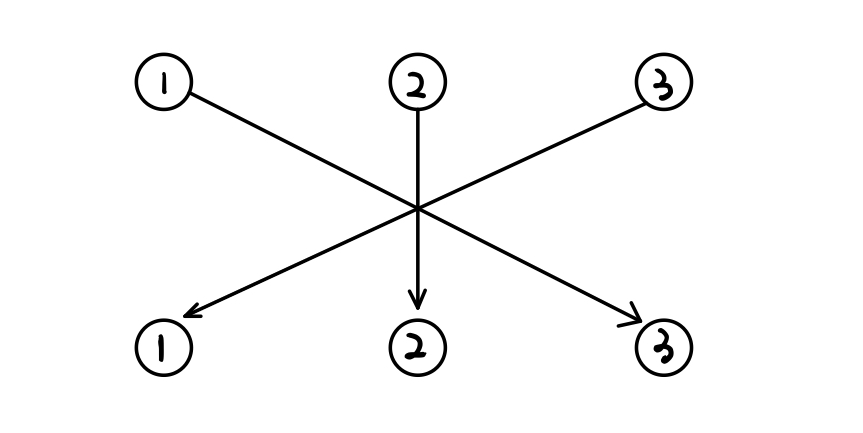
\includegraphics[width=0.5\textwidth]{../../image/twolineperm.png}
      \caption{Two-line notation for permutation \(p=(3\,2\,1)\),in which \(p(1)=3\), \(p(2)=2\) and \(p(3)=1\).}
      \label{fig:figures:twolineperm}
    \end{figure}

\subsection*{One-line notation}

Generally, the first row in two-line notation is a list of set with ascending order, thus, the first line can be omitted and only retaining the second row, which called one-line notation. According to the second line in two-line notation, this notation is \((p(1)\,p(2)\,P(3)\,...)\). This format has occurred more than once in the example mentioned above as (3 2 1).

\subsection*{Cycle notation}

The permutation can be divided into disjoint cycles with the help of applying the permutation to members in set \(S\) again and again. The formula is described as \((x1\,p(x1)\,p(p(x1))\,...)\) which means that the arbitrary element \(x1\) in \(S\) is chose as the start of a cycle and the result \(p(x1)\) would be the next member in the cycle. The third one is applying \(p\) to \(p(x1)\) again. Repeating steps until return the first element . We still using the permutation \(p=(3\,2\,1)\) as example, it has two cycles (1 3) and (2). In the former cycle, the element 1 is applied to the  and we get \(p(1)=3\), after that, the consequence of applying \(p\) to 3 is 1 again, thus, (1,3) is the final result. The same can be proved that (2) is the second cycle. The equation between one-line notation and cycle notation is \(p=(3\,2\,1)=(1\,3)(2)\). The \cref{fig:figures:cycleperm} shows the cycle notation. This notation make a transparent structure of permutation.

\begin{figure}[htb]
  \centering
  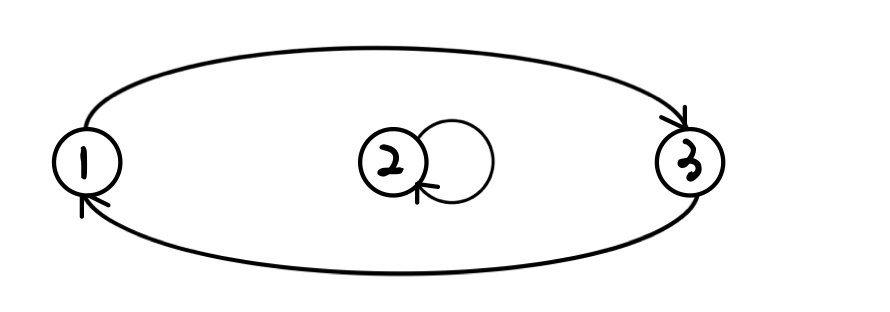
\includegraphics[width=0.5\textwidth]{../../image/cycleperm.png}
  \caption{Cycle notation for permutation \(p=(3\,2\,1)=(1\,3)(2)\).}
  \label{fig:figures:cycleperm}
\end{figure}

\section{Combinatorial maps}

Combinatorial map using oriented subdivided objects to represent the graph embedded in the surface. At the beginning, the concept appeared for the planar graphs of polyhedral surfaces by J. Edmonds \cite{edmonds1960combinatorial} and named as “Constellations” \cite{jacques1969constellations} and “rotation” \cite{ringel2012map} by  A. Jacques and Gerhard Ringel, respectively. The concept is extended from 2-dimensional objects to higher-dimensional objects and called “combinatorial maps” formally.

Sometimes, the computer needs to use data structure to indicate the subdivision of an object and the relation between each of them. The embedded graphs into the surfaces which are assumed to be connected, oriented and compact\cite{nlab:map}, have three typical subdivision, vertices, edges and faces. Each of them are represented by a set of permutations of darts.  

\subsection{Darts}
The combinatorial map is an edges-central model. All edges are divided into two parallel lines with arrow to indicate inverse directions, which called darts or half-edges. The main difference between darts and half-edges is the later one only segment the edges directly without using arrow and parallel lines. The \cref{fig:figures:cycleperm} explain this concept and two formats for it.

\begin{figure}[htb]
  \centering
  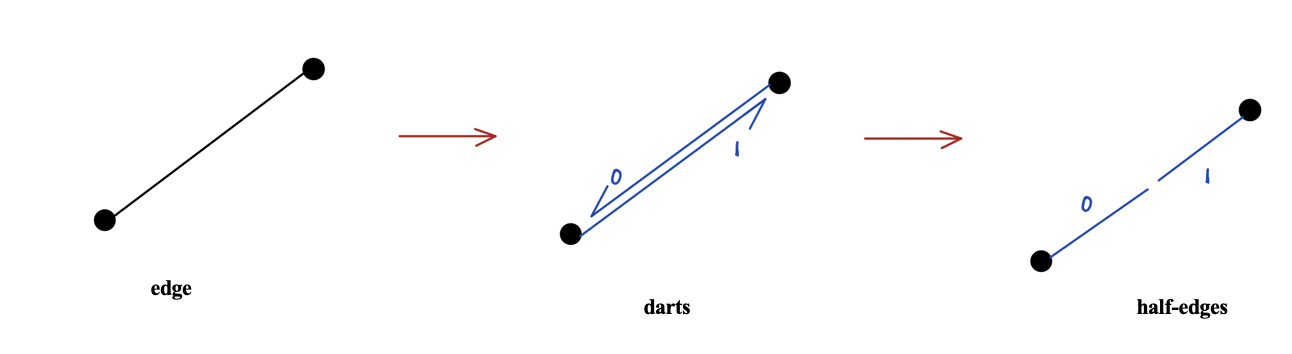
\includegraphics[width=0.8\textwidth]{../../image/darts.png}
  \caption{Two formats of the darts (half-edges) structure.}
  \label{fig:figures:darts}
\end{figure}

\subsection{Edges}
It is obvious that an edges can be represented by a pair of darts. Assume that there is a set of darts \{0,1\} and from the picture we found that dart “0” toward to “1”, on the contrary, dart “1” return to “0”. This means the edges have the orientation for anti-clockwise, it shows a permutation of darts can be used to indicate an edges, as well. One-line notation for the example is (1 0), and convert it to the cycle notation as (0 1). The permutation of edges is denoted as \(\alpha\).

\subsection{Vertices}
A vertex consists of incidence darts surrounding it, which also follows the anti-clockwise and using \(\sigma\) denote this component. As the example in the \cref{fig:figures:vertex}, the vertex can be indicated as (0 1 2) under cycle notation.

\begin{figure}[htb]
  \centering
  
\includegraphics[width=0.8\textwidth]{../../image/vertex.png}
  \caption{The darts surrounding a vertex.}
  \label{fig:figures:vertex}
\end{figure}

\subsection{Faces}
There are two types of faces, the internal faces and the external faces. Both of them are the area surrounded by a series of darts, in other words, both of them have directions. The orientation of the internal faces is clockwise, while for the external ones is anti-clockwise. The signal \(\phi\) is used to indicate the permutation of faces. There are two kinds of faces in the \cref{fig:figures:faces}. (a) has normal faces whose internal face is (0 4 2) and external face is (1 3 5). (b) is a loop which also has the internal face (0) and external one (1). All of the permutations that are mentioned in this section use cycle notation.

\begin{figure}[htb]
  \centering
  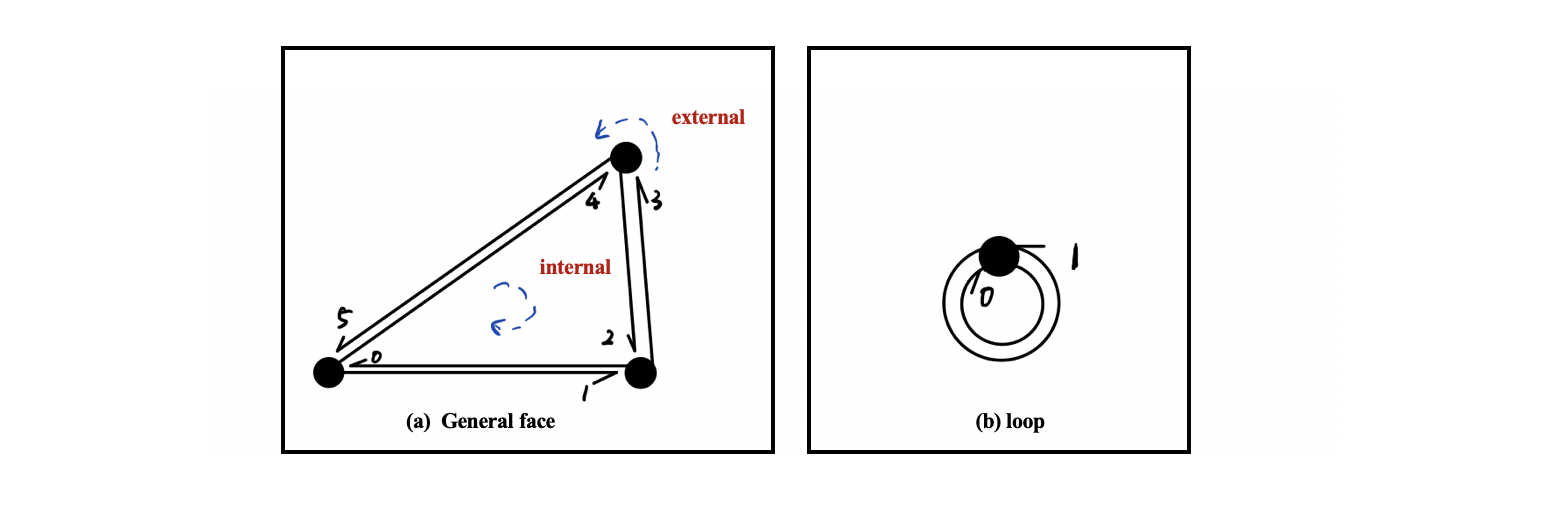
\includegraphics[width=0.8\textwidth]{../../image/face.png}
  \caption{Faces}
  \label{fig:figures:faces}
\end{figure}

\subsection{Planar maps}
Primely, with the requirement of expressing the submission of planar graphs, a compactness topological model  combinatorial map had been utilized. All of  the three component vertices, edges and faces can be tidy and structural represented under an infinite set of darts. \cref{fig:figures:map} draws a typical planar map with format of combinatorial map \(M=(D,\sigma,\alpha)\) in which \(D\) is the infinite set of darts. The length of \(D\) is 14. 

\begin{figure}[htb]
  \centering
  
\includegraphics[width=0.8\textwidth]{../../image/map.png}
  \caption{A classical  combinatorial map for a planar map.}
  \label{fig:figures:map}
\end{figure}

Firstly, the permutation of darts for vertices is \(\sigma=(1\,2\,3)(4\,5\,6)(7\,8)(9\,10\,11\,12)(13\,14)=(2\,3\,1\,5\,6\,4\,8\,7\,10\,11\,12\,9\,14\,13)\) , hence, \(\sigma(1)=2\), \(\sigma(2)=3\),etc. The edges permutation is \(\alpha=(1\,14)(2\,11)(3\,4)(5\,10)(6\,7)(8
\,9)(12\,13)=(14\,11\,4\,3\,10\,7\,6\,9\,8\,5\,2\,13\,12\,1)\) where \(\alpha(1)=14\), \(\alpha(2)=11\),etc. Actually, we have a triple of permutations \(<\sigma,\alpha,\phi>\) on \(D\), and the composition of them is identity, which means \(\phi\alpha\sigma=id\). Accordingly, the permutation of faces is calculated as \(\phi=\sigma o \alpha=(1\,11\,13)(2\,4\,10)(3\,14\,12\,8\,6)(5\,7\,9)\).

The orientation of each component is a quite strict constrain to define a combinatorial maps. The definition for discussing whether two maps are conjugation equivalent is only if they are isomorphic by a homeomorphism of the underlying surfaces. That is to say, judging the equivalent of two maps relies on if corresponding parts of those are obey the same rotation, rather than they have the same number of elements for the each component. In the \cref{fig:figures:equivalent}, although the three combinatorial maps have the same number of vertices, edges and faces, the first two a equivalent, and the last one is not the same with them.

\begin{figure}[htb]
  \centering
  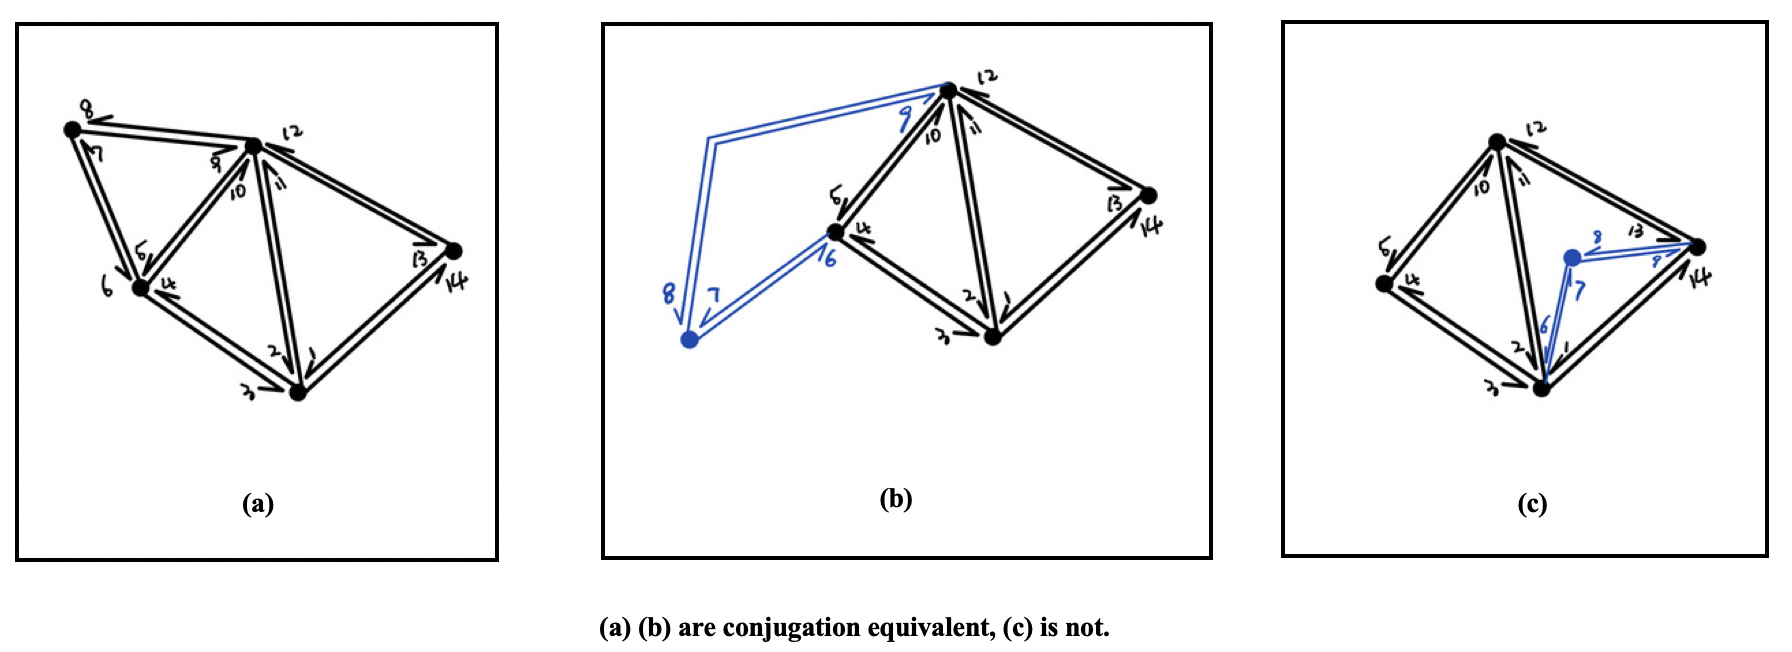
\includegraphics[width=0.8\textwidth]{../../image/equivalent.png}
  \caption{The equivalent of the combinatorial maps.}
  \label{fig:figures:equivalent}
\end{figure}

\subsection{Genus}
An orientable surface might have “holes” , and the number of “holes” it has called genus. For example, sphere as (a) in \cref{fig:figures:orsurfaces} has 0 genus and torus as (b) which looks like a donut has 1genus. The genus \(g\) of a surface which the graph embedded in can be computed by the Euler-Poincaré formula \cite{richeson2008euler}:\(V-E+F=2-2g\). The \(V\), \(E\) and \(F\) are the number of vertices, edges and faces in the embedded graph, respectively. Substituting , \(V\), \(E\) and \(F\) in the equation for features of combinatorial map as \(c(\sigma)-c(\alpha)+c(\phi)=2-2g\). The \(c\) is the function to calculate the count of the cycles for each component.

\begin{figure}[htb]
  \centering
  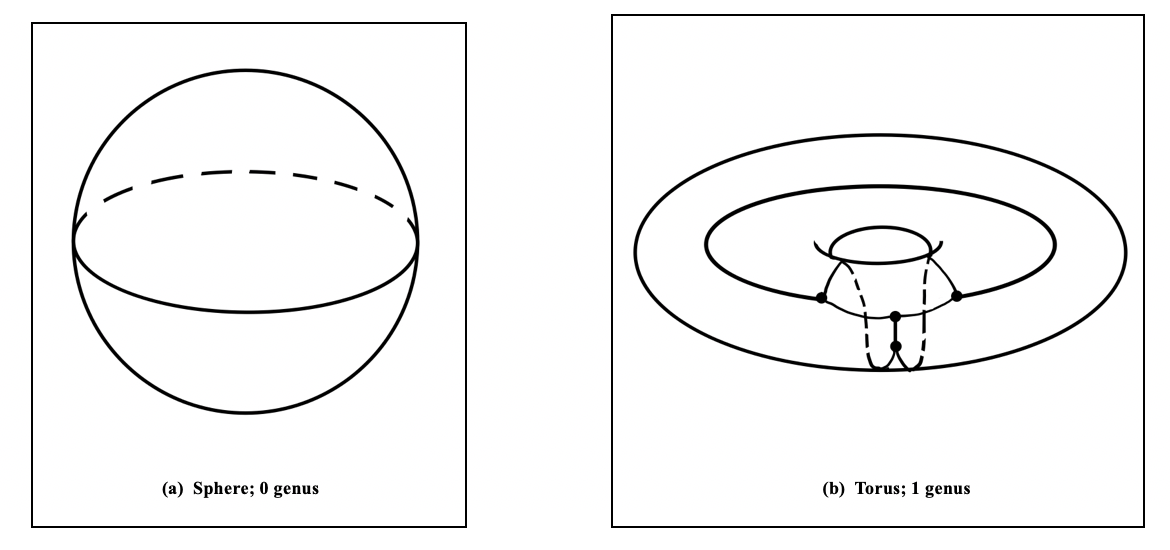
\includegraphics[width=0.8\textwidth]{../../image/oritation surface.png}
  \caption{Two oriented surfaces.}
  \label{fig:figures:orsurfaces}
\end{figure}

\subsection{Generalised maps}
Planar graph is the graph embedded in a plane surface which has 0 genus. It is a crossing free model and the combinatorial map for it is also named 2-dimensional map. Gradually, the combinatorial map is discovered not only to represent the planar maps, but to indict more complicate objects with higher-dimension, even the non-orientation surfaces. The triple of permutations \(<\sigma,\alpha,\phi>\) on set \(D\) is still used to describe the subdivision of the objects.  Take the torus as the example, in \cref{fig:figures:hdmap}, the embedded graph on this oriented surface drew like (b), and the labels are half-edges. The permutation for edges is  \(\alpha=(1\,8)(2\,11)(3\,4)(5\,12)(6\,7)(9\,10)\) and for vertices is \(\sigma=(1\,2\,3)(4\,5\,6)(7\,8\,9)(10\,11\,12)\). (c) is the isomorphic map for the graph.

\begin{figure}[htb]
  \centering
  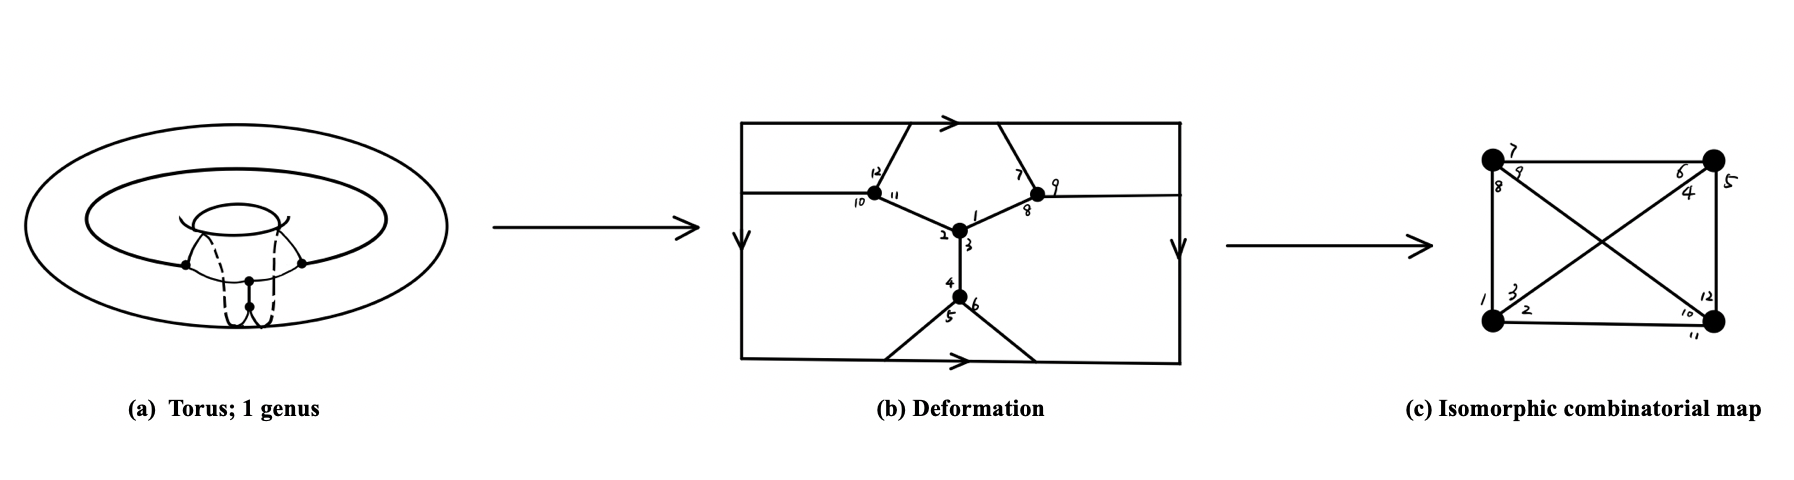
\includegraphics[width=0.8\textwidth]{../../image/hdmap.png}
  \caption{Combinatorial map for torus.}
  \label{fig:figures:hdmap}
\end{figure}

As far, the combinatorial maps can be used to indict a lot of objects with tidy and direct structure. It also involve into the field of graph drawing and hierarchical image partitioning \cite{haxhimusa2005hierarchical}. Some graph algorithm library like Pigale \cite{de2002pigale} use the structure as the basic data structure.
\include{content/2-Relatedwork}
% !TeX encoding=utf8
% !TeX spellcheck = en-US

\chapter{Specification}

\section{Calculating of combinatorial maps}

\subsection*{Parsing the user input which is limited to the cycle notation.}

\textbf{Correctness} The input can be parsed into the valid cycle notation of each permutation.

\textbf{Reliability} The tool can check the inputs at any time. If the input is illegal, there will be a space to show the warning information and the correct format of the input. All others operations must after checking and parsing the input.

\textbf{Performance} The correct result of parsing will display in the form of text and image.

\subsection*{Transforming cycle notation to one-line notation.}

\textbf{Correctness} These two notations can be converted to each other.

\textbf{Performance} The correct result will display in the form of text and image.

\subsection*{Computation of faces by given the permutations of vertices and edges. This particularly depends on the equation \(\phi=\sigma o\alpha\).}

\textbf{Correctness} Any of three component can be educes by others, i.e.,\(\phi\alpha\sigma=id\).

\textbf{Performance} The cycle notation and one-line of face will display in the form of text and image.

\subsection*{Generating a random combinatorial map by only given the number of darts (and vertices).}

\textbf{Correctness} The graph should be connected, and the composition of permutations must be identity.

\textbf{Performance} Showing each component with text and image.

\section{Visualising combinatorial maps}

\subsection*{The tool using different methods to visualise the combinatorial maps.}

\textbf{Correctness} The maps must be followed the constraints of the maps, that is, it must obey the orientation of each part. For the planar map, it must avoid the cross as much as possible. The whole structure must be connected and filled in the specific area without overflow.

\textbf{Clarity} User can have a clear mind when they look at the images. Each element must be discovered directly rather than distinguished for a long time.  Especially the edges should not be cramped together and have an explicit identity.

\textbf{Performance} Showing the results in the right area and have an effective introduction. The result must show in the limited time.

\textbf{Consistency} The result of the certain method for a map must be the same at any time. This requires the methods must be stable and robust. Otherwise, the results might confuse the users and they will misunderstand about the combinatorial maps.

\textbf{Aesthetics} The whole tool must have a clear structure and comfort colour matching. The layout of the visualisation must be reliable. A good interface and drawing will attract user exploring more about the combinatorial maps.

\section{Knowledge of combinatorial maps}

\subsection*{The tool aims to pass more information about combinatorial maps for whether they are beginners or experts in the relative area.  A introduction of the maps and tool is necessary.}

\textbf{Correctness} The background of the combinatorial maps must be correct which cannot be misleading.

\textbf{Performance} A introduction page to describe the tool and the structure. Other information like genus number can be shown in the visualisation part.

% !TeX encoding=utf8
% !TeX spellcheck = en-US

\chapter{Implementation}

This section covers the two parts, the implement for visualisation of combinatorial maps and package them as a tool.

\section{Language}

For designing the application as a tool, the JAVASCRIPT is used to the implement all the function. Therefore this  is a website tool which is convenient for people to search no matter when and where they are. A library called D3.js \cite{bostock2015d3} is used to draw image as format of SVG.

\section{Visualisation Methods}

The methods are still concentrate on the layout for drawing a combinatorial maps. The features of the maps are discovered as the base sketch for the completely graphical model. The base data structure of  the permutation is array, that is, all types of the permutations are kept as array and note the cycle notation as \(*C\) and one-line notation as \(*P\). For example, a permutation of vertices is (1 0 3 2), \(VC=[[0,1],[2,3]]\) and \(VP=[1,0,2,3]\) are cycle notation and one-line notation of it , respectively.

\subsection{Tree Based Method}

\subsubsection{Spanning trees}
The spanning tree is general subgraph of connected graphs. There are two kinds of spanning tree, one contains the maximal edges of the maps without cycles, and another one connects all the vertices through a single path. It is obvious that there is not only one spanning tree of a map.

\begin{figure}[htb]
    \centering
    
\includegraphics[width=0.8\textwidth]{../../image/spanning tree.png}
    \caption{The spanning tree of a combinatorial maps.}
    \label{fig:figures:spantree}
  \end{figure}

\subsubsection{Depth First Searching Algorithm}
Depth first searching algorithm(DFS for short) is a route from an arbitrary vertex to another one. In this problem the DFS is used to find the spanning trees of the maps and validate whether the structure is connected or not. The start point is the vertex who has the least valued dart. There are some steps for DFS in this problem:

  \begin{itemize}
    \item[a)] Using five list for storing the unsearched vertices \(V\) and darts \(D\) , as well as recording the possible searching path \(P\) including the first element of \(V\) (removing the element from , as well) and valid path via all vertices \(PV\) or some edges \(PE\). An assistant array \(DTV\) is used to record corresponding vertices of darts.
    \item[b)] Pop out the last element \(s\) in \(V\) as the start point of the current segment.
    \item[c)] If all darts of the  have been searched, continue from step b).
    \item[d)] Otherwise, push \(s\) in \(P\) again. Find the first unsearched dart \(d_s\) in \(VC[s]\) (cycle notation for vertices permutation), and get the next dart \(d_t\) via (one-line notation for edges permutation), so that the target vertex \(t\) is \(DTV[d_t]\). Delete \(d_s\) and \(d_t\) in \(D\).
    \item[e)] If \(t\) is in \(V\), remove it and push the new path in \(PE\) and \(PV\), as the same time, add \(t\) to the tale of \(P\).
    \item[f)] Repeat the steps b) to e) until any one of \(V\), \(D\) and \(P\) is empty.
    \item[g)]If \(V\) is empty, return the truth result with \(PE\) and \(PV\), else, return false and other results are empty. 
  \end{itemize}

  \newpage
  \begin{figure}[htb]
    \centering
    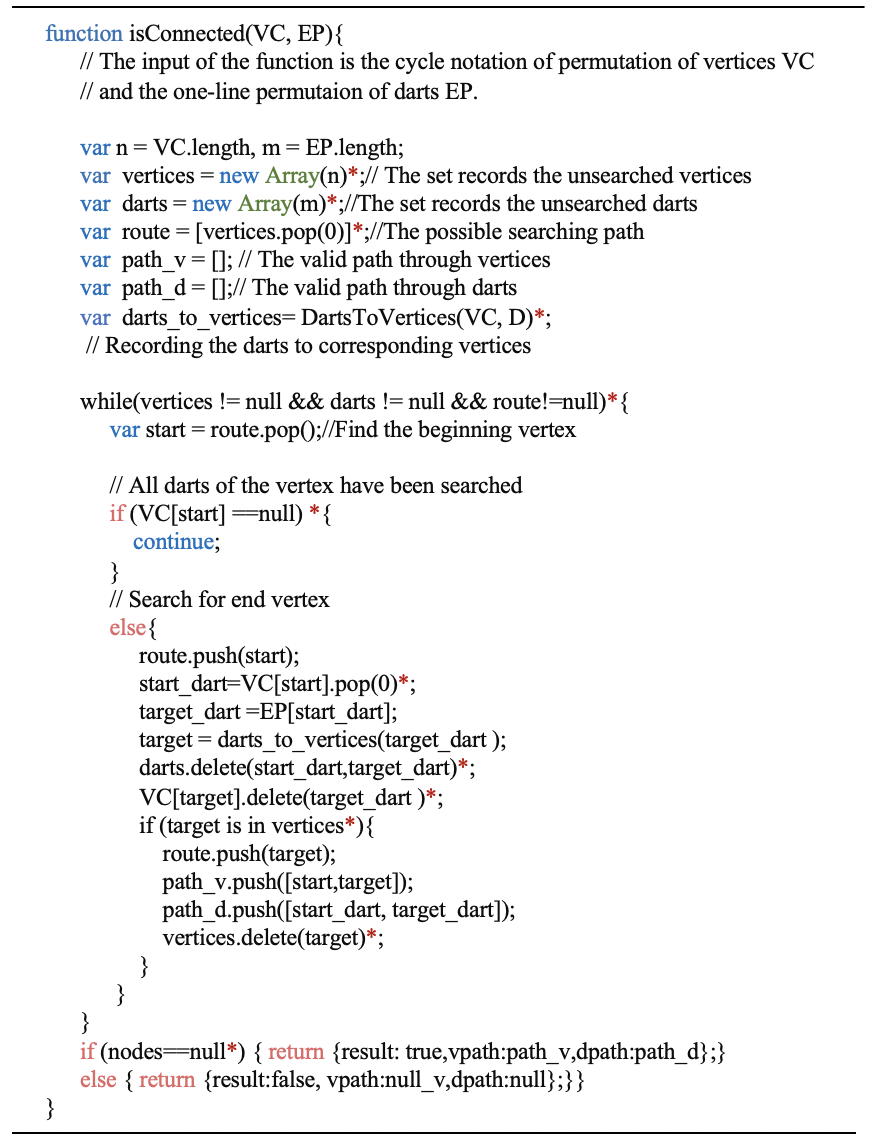
\includegraphics[width=1\textwidth]{../../image/DFS.png}
    \caption{The rough implementation of DFS by JAVASCRIPT, the lines with \textcolor[RGB]{176,35,24}{*} are not the standard JAVASCRIPT code.}
    \label{fig:figures:DFS}
  \end{figure}

\newpage
\subsubsection{Tree drawing algorithm}
Recent paper by Christoph Buchheim et al \cite{buchheim2002improving} introducing a method for drawing a n-ary trees with \(O(n)\) time complexity. It is an improvement of the method for drawing binary trees proved by Edward Reingold and John Tilford \cite{reingold1981tidier}. Bill Mill’s article \cite{milldrawing} described the evolution of the algorithm. There are six principles should be considered when draw a tree:
\begin{itemize}
    \item[a)] The edges cannot be cross with each other.
    \item[b)] The nodes in the same depth should be kept in the same height.
    \item[c)] The whole tree should be as narrow as possible.
    \item[d)] The vertical position of parent nodes is the middle of their children.
    \item[e)] Wherever the subtree lies in a tree, it should move the same distance with its parents.
    \item[f)] For the n-ary tree, the children should divide the space evenly for their parents. 
  \end{itemize}

  For obeying the first four principles, the algorithm searches the tree from bottom to up for settle the nodes, namely, post-order traversal of the tree. When maintain the fourth principle, the parent nodes move to right and the right child of it should move toward right also, which leads to a bad result that right children in a node will cover the left children of the later nodes, in another word, some of the nodes will be disappeared. The principle e) aims to solve the problem. In order to achieve the principle, the concepts of mod, contours and threads had been proposed. The mod records the distance that the current tree should be moved, and then, moving each tree with the accumulated mod value from its ancestors to itself. This concept can solve the problem mentioned above, but it cost the running time as it needs two times to search the tree. The contours and threads make the algorithm less complexity, which looks each subtree as a block.The contour is the leftmost side of trees (minimum x-coordinate) called \textit{left contours} or the rightmost side of trees(maximum x-coordinate) called \textit{right contours} as the example in the \cref{fig:figures:subtree}. The threads are the link in the contours if the two nodes have no relationship.

  \begin{figure}[htb]
    \centering
    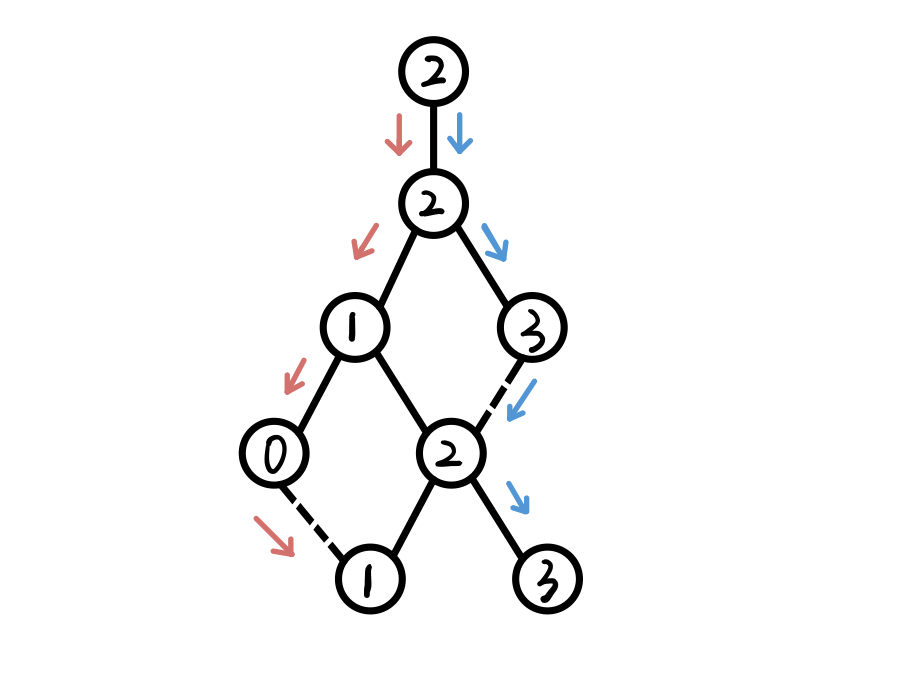
\includegraphics[width=0.8\textwidth]{../../image/subtree.png}
    \caption{The red lines show the left contour [2,2,1,0,1], and blue lines are right contour [2,2,3,2,3]. The dash lines are the threads.}
    \label{fig:figures:subtree}
  \end{figure}
  \newpage
  The thread can reduce the complexity and avoid the conflict between the subtrees, which helps to calculate accumulated mod value during the first walk of the tree. The last principle is specifically set for the n-ary tree. Since each parent might has more than two children, the left contour and right contour cannot totally deal with the conflict the problem. The concept of the ancestor is used to decide which left siblings conflicts with current subtree.

  \begin{figure}[htb]
    \centering
    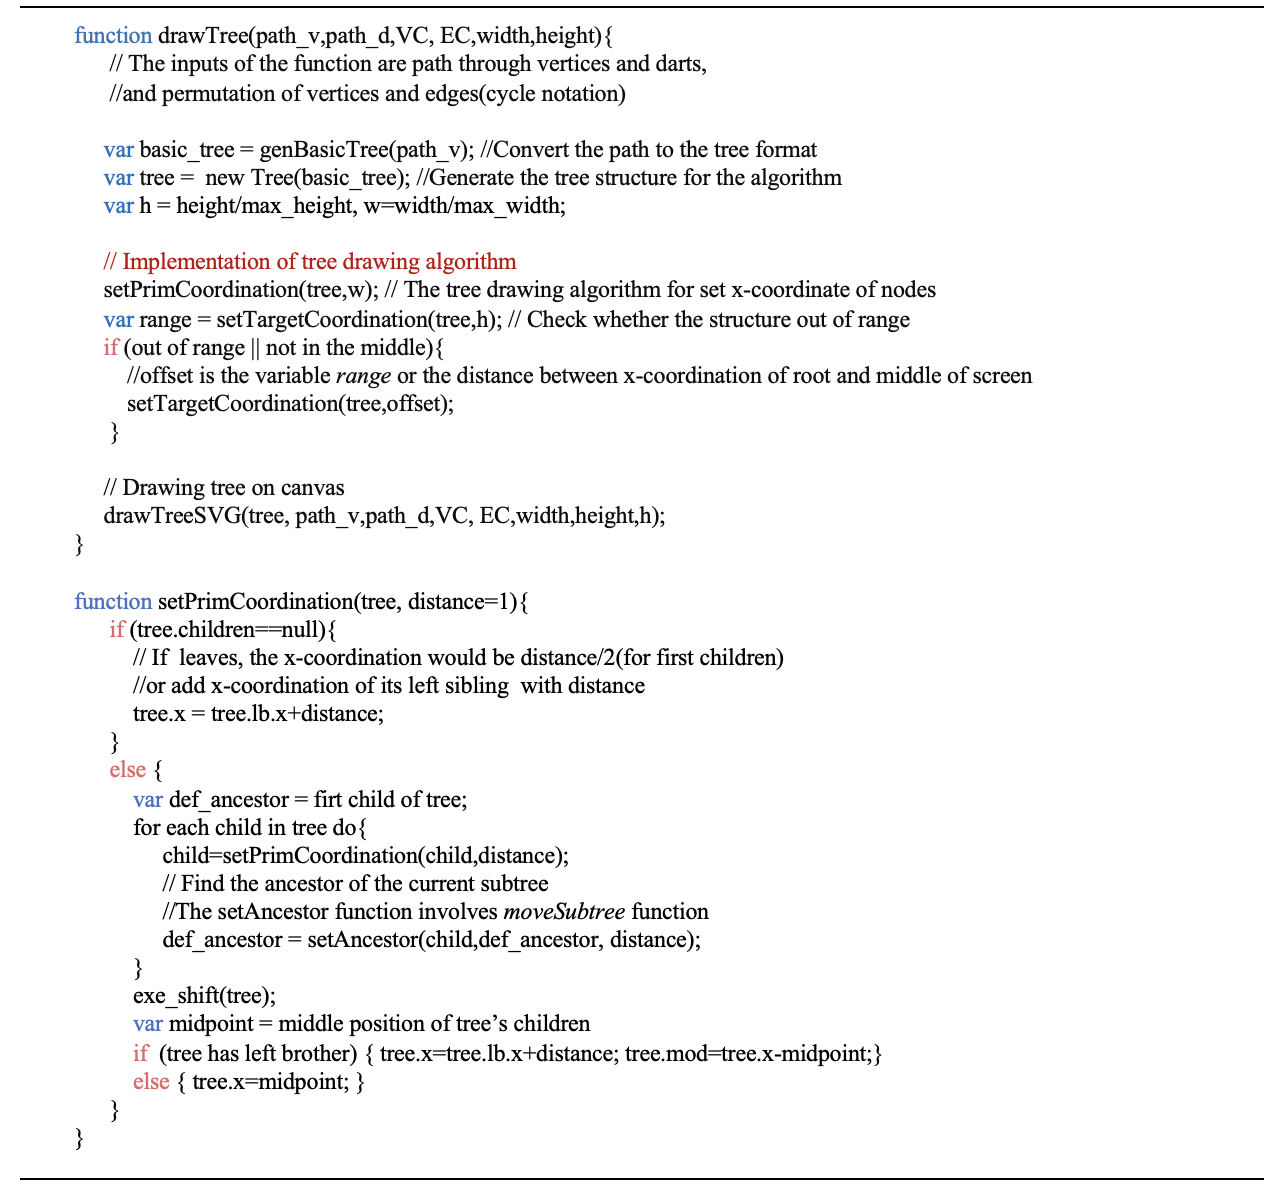
\includegraphics[width=1\textwidth]{../../image/drawtree.png}
    \caption{The constructor of tree drawing function and tree drawing algorithm in the JAVASCRIPT implementation.}
    \label{fig:figures:drawtree}
  \end{figure}

  \newpage
  The tree drawing algorithm just concerns on how to calculate the x-coordination, rather than fill the structure into a certain canvas. It is necessary that computing the vertical and horizon gap between each nodes. The horizon gap can be calculate directly, just using height of canvas divided by max depth of the tree. The vertical gap can be conducted by the same way, while, it is more difficult to compute the max width for the tree. The weighted average method is used to solve the problem. Firstly, generating a list \textit{wide} which records the width for each level of trees. Sorted \textit{wide} with ascending order as the next step. Finally, the weight of each item in \textit{wide} is the serial number of the item divided by the length of \textit{wide}, and the computing the weighted average of items. 

  The function \textit{drawTreeSVG()} in \cref{fig:figures:drawtree} is to do the drawing work on the canvas with D3.js. The coordination of the nodes and the path of links should be collected as a list, after that, drawing the model in a specific area. The \cref{fig:figures:treedraw} shows the result of the implementation of tree drawing algorithm.

  \begin{figure}[htb]
    \centering
    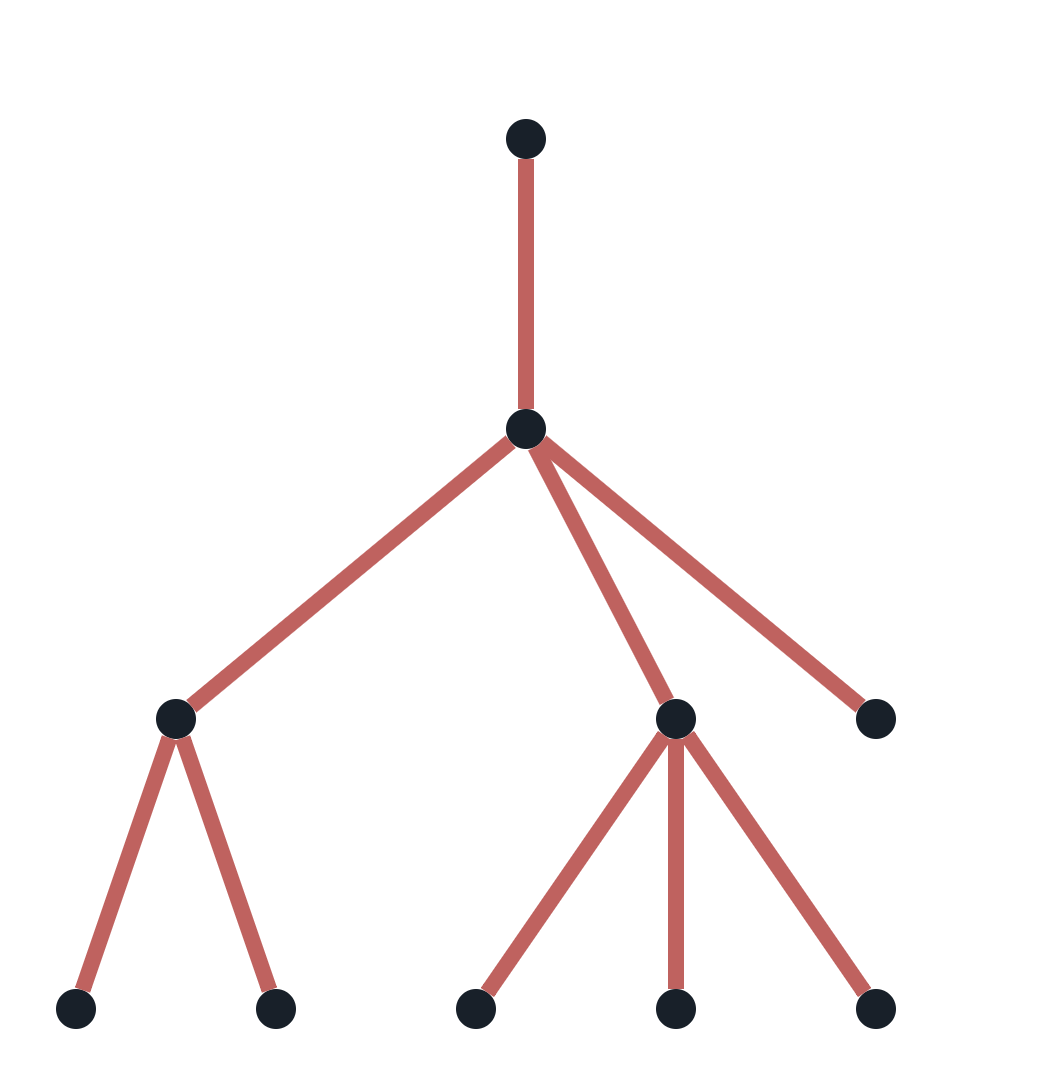
\includegraphics[width=0.6\textwidth]{../../image/treedraw.png}
    \caption{Result of the algorithm.}
    \label{fig:figures:treedraw}
  \end{figure}
  \newpage
  We have already got the tree sketch of the combinatorial maps. Some of darts are fixed within the tree structure, while the rest should be settled according to the existed darts. It uses the same approach to calculate the coordination of the endpoints of remaining darts in \textit{vertices based method}. 

  \begin{itemize}
    \item[a)] Find two darts around the same vertices.
    \item[b)] If there is no darts between them, return a).
    \item[c)] Otherwise, calculate the angle between them using \(angle=atan2(v1.y,v1.x)-atan2(v2.y,v2.x)\) ( and \(angle=angle+2*\pi\) , if \(angle<0\)).
    \item[d)] \(N\) is the number of darts between them, and the radian \(rad\) between each nodes is the \(angle/(N+1)\). The less valued darts is seen as the base line, and \(v1\) is the direction vector for base line.
    \item[e)] For \(n=1 \, to\, N\), \(d_n.x=v1.x*cos(rad*n)+v1.y*sin(rad*n)+v.x\) and \(d_n.y=-v1.x*sin(rad*n)+v1.y*cos(rad*n)+v.y\) where \(v\) is the vertex which the darts surrounding.
    \item[f)] Repeat the above steps until all the darts are placed. 
    \item[g)] Connect the new darts rely on the permutation of edges.
  \end{itemize}

  \subsubsection{Bezier curves} 
  For the purpose of  receiving a sleek and smooth edge, the connection using curve line rather the straight. Bezier curve is an algorithm to calculate a curve between to endpoints. Unlike other splines, the Bezier curve must through the start and target points. The degree of curvature depends on the control point. Second-order Bezier curve has one control point and third-order Bezier curve has two.  In this method, the third-order Bezier curve is being used. The control points are the extending along the direction of corresponding darts.

  \begin{figure}[htb]
    \centering
    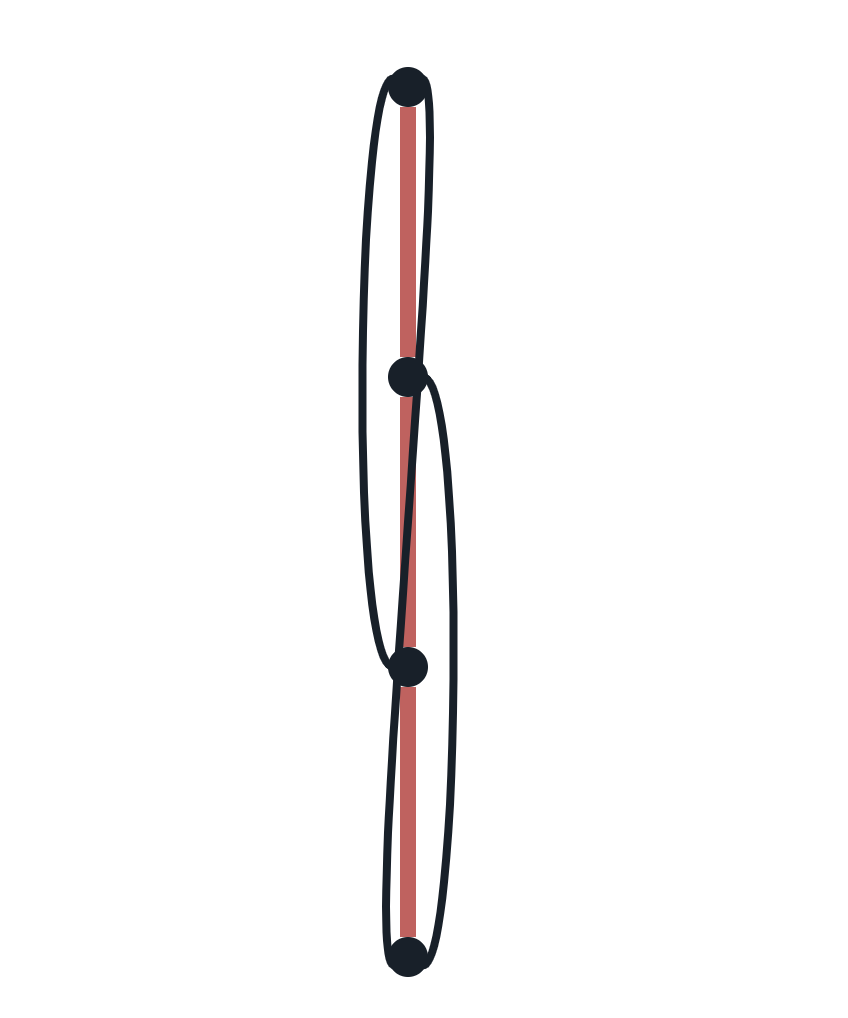
\includegraphics[width=0.5\textwidth]{../../image/example1.png}
    \caption{Result of the method for visualisation of the combinatorial map about Planar Tetrahedron(planar map).}
    \label{fig:figures:example1}
  \end{figure}

  \subsubsection{Problem}
  The result in \cref{fig:figures:example1} is a planar maps. It has been mentioned that the planar maps is a cross-free model, while in the \cref{fig:figures:example1}, the crossing occurs. As the same time, for the Petersen graph in the \cref{fig:figures:pertersengraph1} has 2 genus, which means that it is not necessary to avoid the cross as much as possible. 

  \begin{figure}[htb]
    \centering
    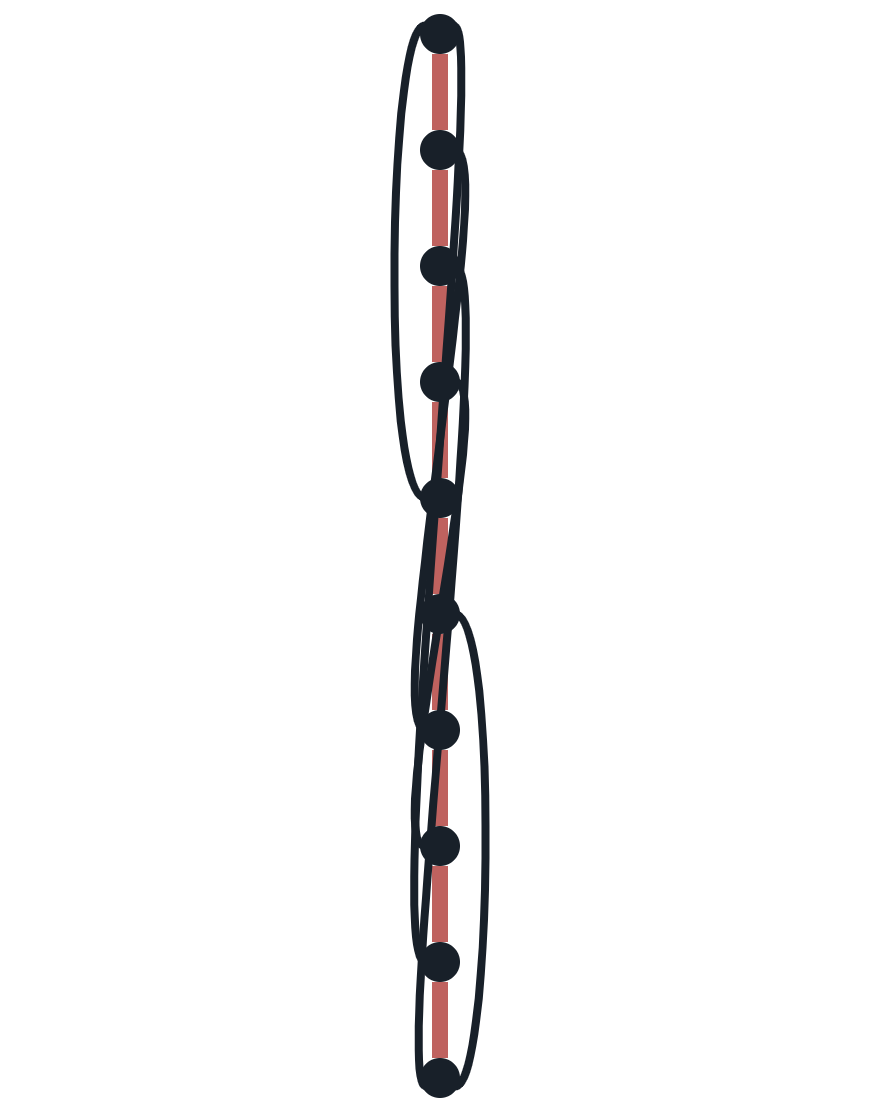
\includegraphics[width=0.4\textwidth]{../../image/pertersengraph1.png}
    \caption{Result of the method for visualisation of the combinatorial map about Petersen graph.}
    \label{fig:figures:pertersengraph1}
  \end{figure}

  However, the edges look so mass and entangled that every edges cannot be read directly. The traditional way is label the corresponding number in the end of each half-edges but this makes the image more disordered and unclear. The tips and highlight are added to indicate each vertices and edges like \cref{fig:figures:highlight}.

  \begin{figure}[htb]
    \centering
    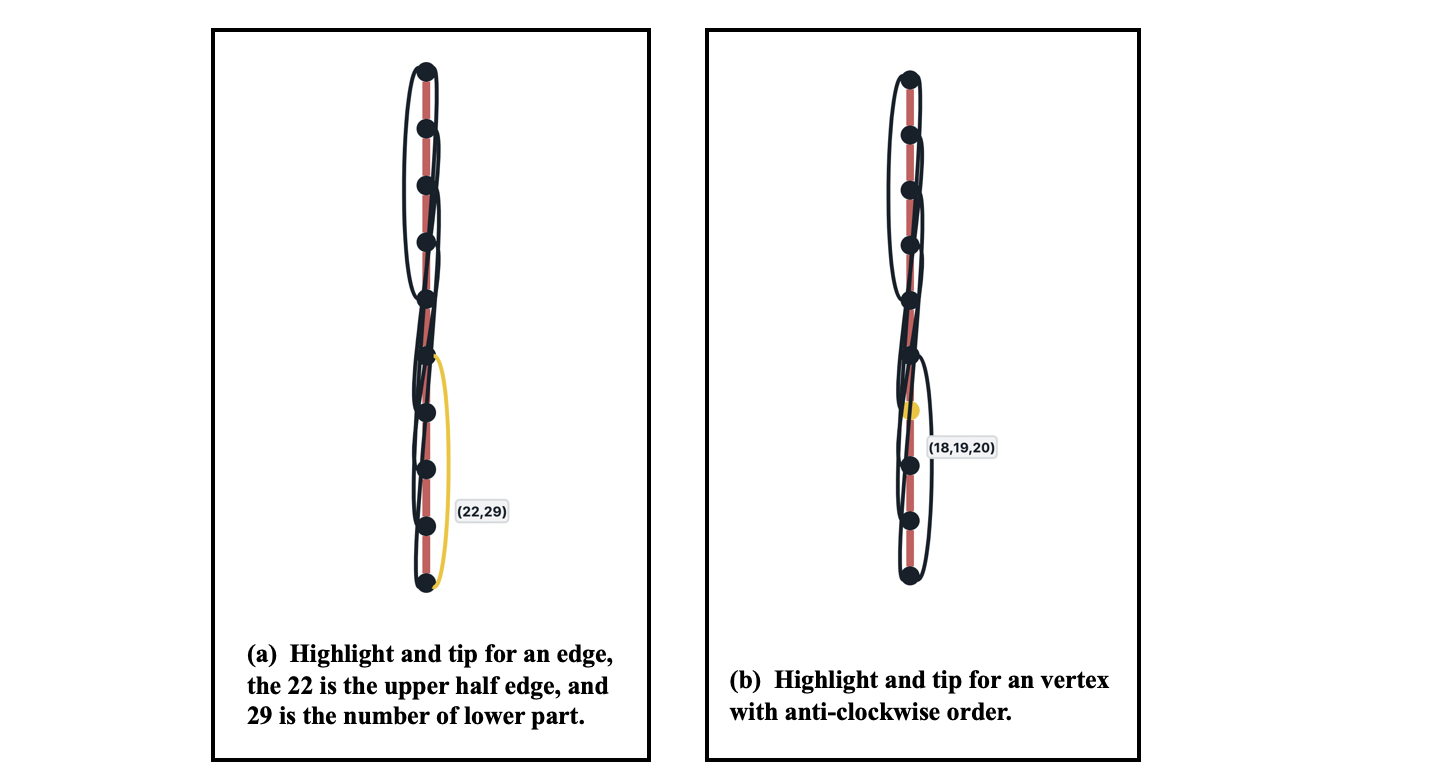
\includegraphics[width=0.8\textwidth]{../../image/highlight.png}
    \caption{The tips and highlights example.}
    \label{fig:figures:highlight}
  \end{figure}

  \subsubsection{Improve version}
  The main issue about hardly avoiding the cross for planar map is the position or direction of darts around a vertex. The spanning trees (as the result of DFS algorithm) of most combinatorial maps are a straight line, like the red part in the examples. When settle the extra darts , in the previous method, it is just divide the angles between excited darts. This leads to absolutely opposite directions for a two darts which should be connected. Therefore, the result of the connection using Bezier curve will through the middle line rather than cross the line.

  On behalf of improving the darts angle problem, an idea is to involve the darts as virtual nodes into the tree structure. That is to say, each vertex has darts essentially and it might also have children in the spanning tree structure, so as to drawing the darts as the virtual children for a vertex in the tree structure. After that, one or some of the darts are connect to the other darts who are belongs to the children vertices of the current one in the original tree model. The \cref{fig:figures:improbvetree} shows the transformation. The circles filled white are types of virtual nodes, one is the joint of two darts in the tree structure, and another one is the darts of the vertices.

  \begin{figure}[htb]
    \centering
    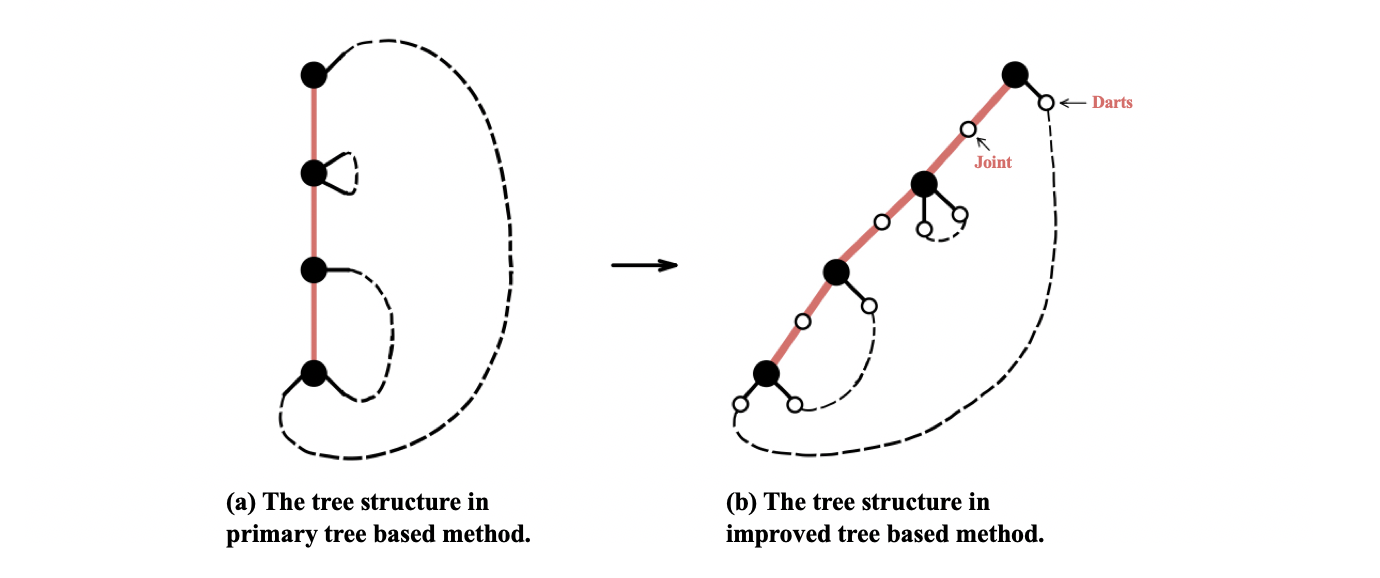
\includegraphics[width=0.8\textwidth]{../../image/improbvetree.png}
    \caption{The compare between tree structures in two methods.}
    \label{fig:figures:improbvetree}
  \end{figure}

  Redefining the tree structure is not enough to avoid the cross, some situation of the connection have to discuss too. (Note: Reverse direction of a dart in all situations means doing the mirror inversion according to the \(x=x_d\) where \(x_d\) is the x-coordination of the dart.)

  \begin{itemize}
    \item[a)] If the less x-coordination node towards left and larger one to the right, the curve should through the bottom.
    \item[b)] The extension of two darts are cross. This station still arrives the bottom but the direction of both are reversed.
    \item[c)] If any of the two darts is the middle children of its father, the direction of the middle dart is horizon.  This connection also go via bottom.
    \item[d)] The last situation is both darts are toward the same direction. For the right side, if the less y-coordination node has larger x-coordination, reverse the lower node and connect them through the bottom, otherwise, the connecting line will go through the middle node of two darts. It is the same for the right side.
    \item[e)] Last but not least, counting the numbers of connections through bottom, left and right, respectively. Using corresponding lines to divide the each space. All are using 3-order Bezier curves.
  \end{itemize}

  \begin{figure}[htb]
    \centering
    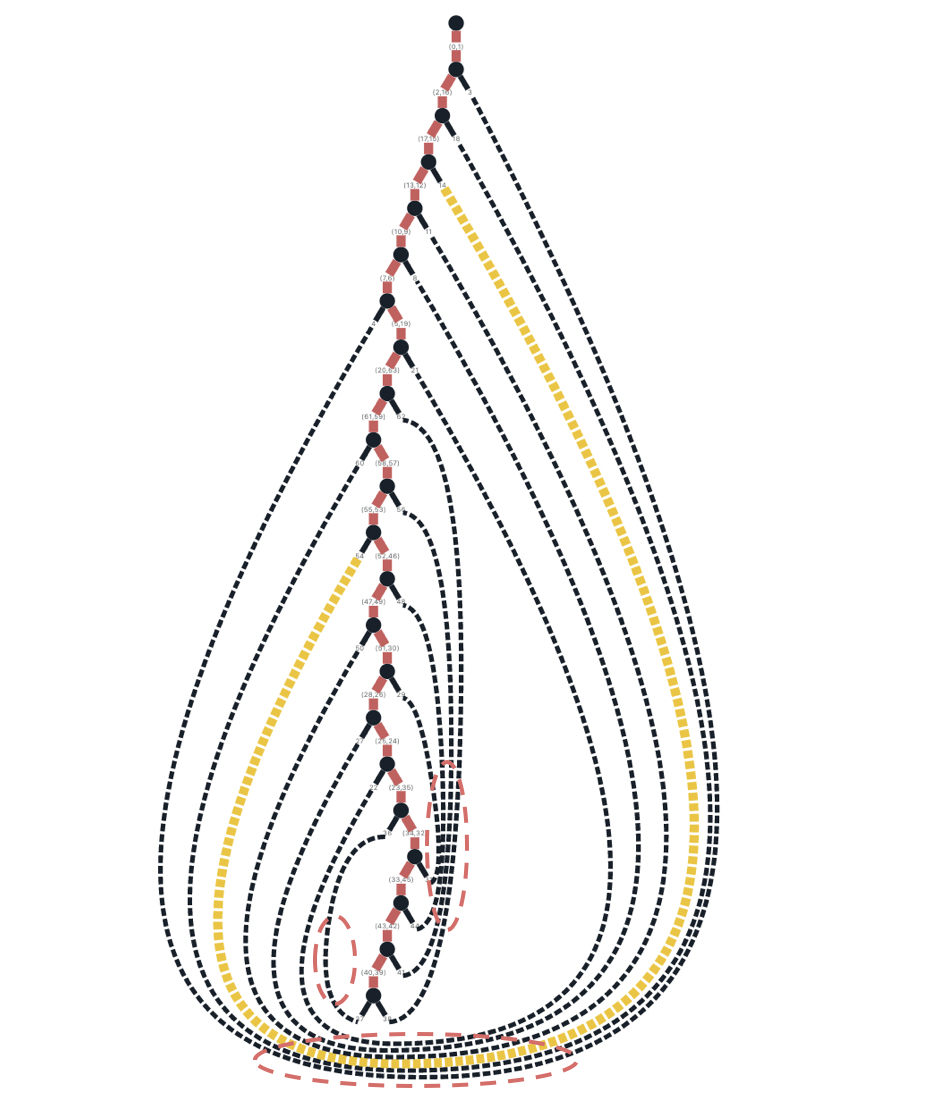
\includegraphics[width=0.6\textwidth]{../../image/improvemap.png}
    \caption{The result of improved tree based method for rooted dodecahedron graph.}
    \label{fig:figures:improvemap}
  \end{figure}

  This method has greatly reducing the cross, and the oval with dash line demonstrate the essence of the ideas. As the mean time, it do not need extra time to calculate the position of darts which out of the tree structure. Due to dividing the fix size of the area, the gap between lines are narrow. Highlight the selected line can produce a simple and convenient recognition of it.

  \subsection{Face Based algorithm}
  This approach comes from the dual of map. If it succeed, it might recover the surfaces which the  combinatorial maps embedded in.

  \subsubsection{Dual}
  Any embedded graph has its dual graph in the same surface. The vertices of the dual structure is the centre of the corresponding faces in the combinatorial map. The darts around the vertices in the dual map are the darts surrounding the primary faces.

  \begin{figure}[htb]
    \centering
    
\includegraphics[width=1\textwidth]{../../image/dual.png}
    \caption{The dual map of  a combinatorial map.}
    \label{fig:figures:dual}
  \end{figure}

  The core of the idea which comes from this structure is generating every faces of the combinatorial maps. Gluing the faces together by connecting the corresponding darts under the edges permutation. With the help of folding algorithm, the drawing results are improving from 2-dimensional to 3-dimensional which shows the underlying surfaces that the maps embedded in.

  \subsubsection{Visualisation}
  The fundamental task is to drawing the faces without gluing. It is necessary that separating the screen into \(N_f\) parts where \(N_f\) is the number of faces. Firstly, judging whether the \(N_f\) can be squared. If possible, the result is denoted as \(n_l\), and the screen splits into \(n_l\) rows and \(n_l\) columns. If it is not , dividing the canvas into 3 lines and \(abs(N_f/3)+1\) columns. The next step is drawing each faces, it is easy to find that each face is a polygon, bilateral(with two vertices) or loop(with one vertex).

  \begin{figure}[htb]
    \centering
    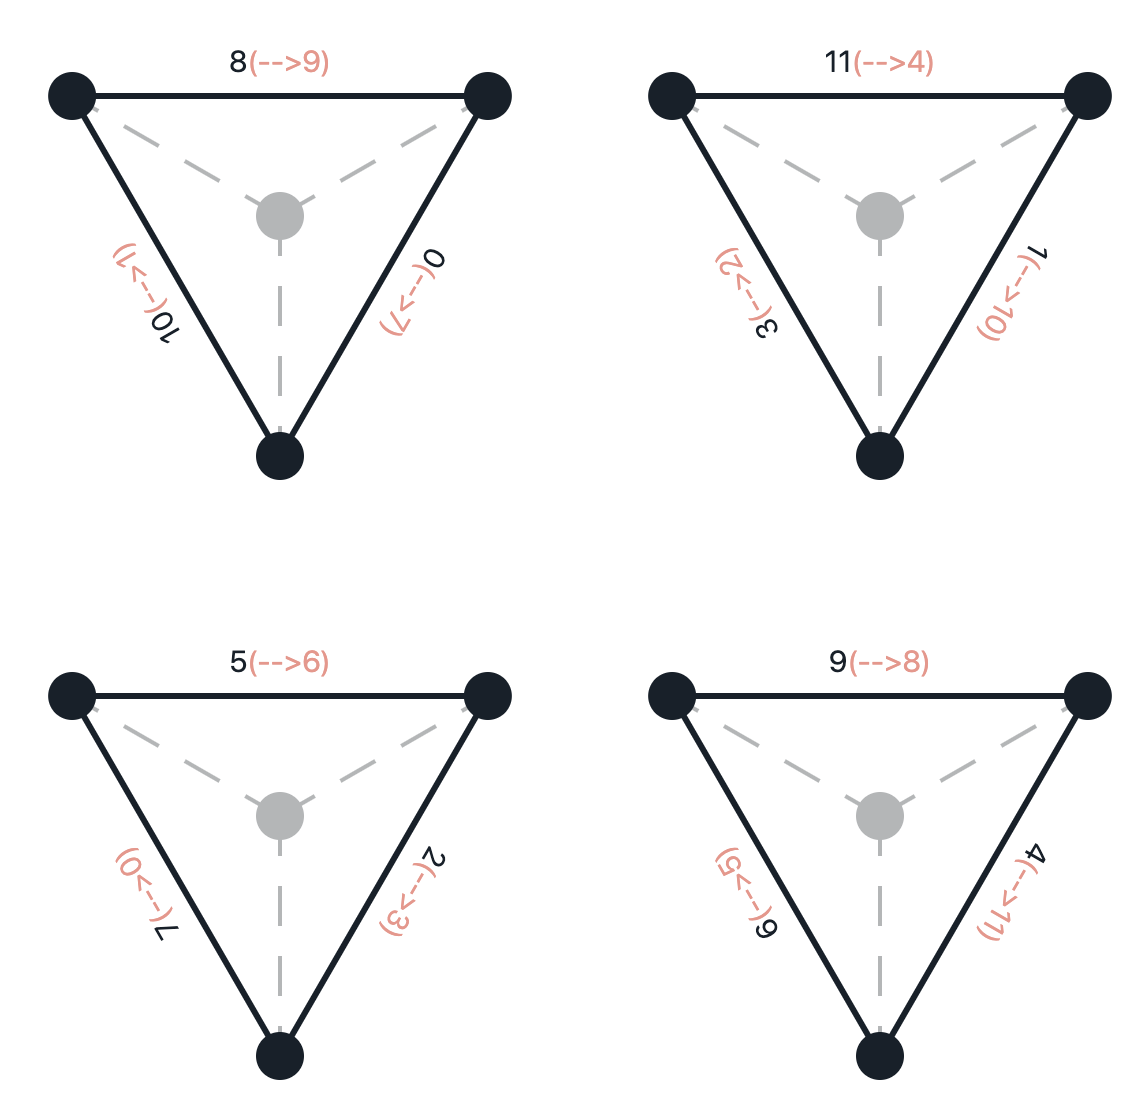
\includegraphics[width=0.5\textwidth]{../../image/facesmap.png}
    \caption{The visualising of a combinatorial map for planar tetrahedron by faces based method.}
    \label{fig:figures:facesmap}
  \end{figure}

  The labels of the darts are the darts number (black words) and the red numbers indicate which darts to connect with. The grey nodes and dash lines are the corresponding parts in dual maps.

  \section{Tool Structure}

  A tool aims to package the methods for visualisation of combinatorial maps as a website application. This section covers the structure of the tool including two pages: introduction and visualiser, as well as introducing how does each section work. The style for the layout of pages uses Bootstrap.css \cite{bootstrap2019}, and the icon in the pages also from the bootstrap opening icon set \cite{openicon2019}.

  \subsection{Introduction}
  The purposes of the tool are not only displaying the combinatorial maps, but also helping the researchers or beginners reward the knowledge of it. Therefore, an introduction page is necessary to deliver the basic background of maps, the features which the visualiser involved, and the other informations for example what algorithm are implemented. This is also seen as the starting page.

  \subsubsection{Head}
  The head of the page is to describe why the tool should be created and provide the links. The right button ‘Get start’ goes to the visualiser page if people want to experience the tool directly, while the left one stays at the local page to let people learn more about the theory knowledge.
  
  \begin{figure}[htb]
    \centering
    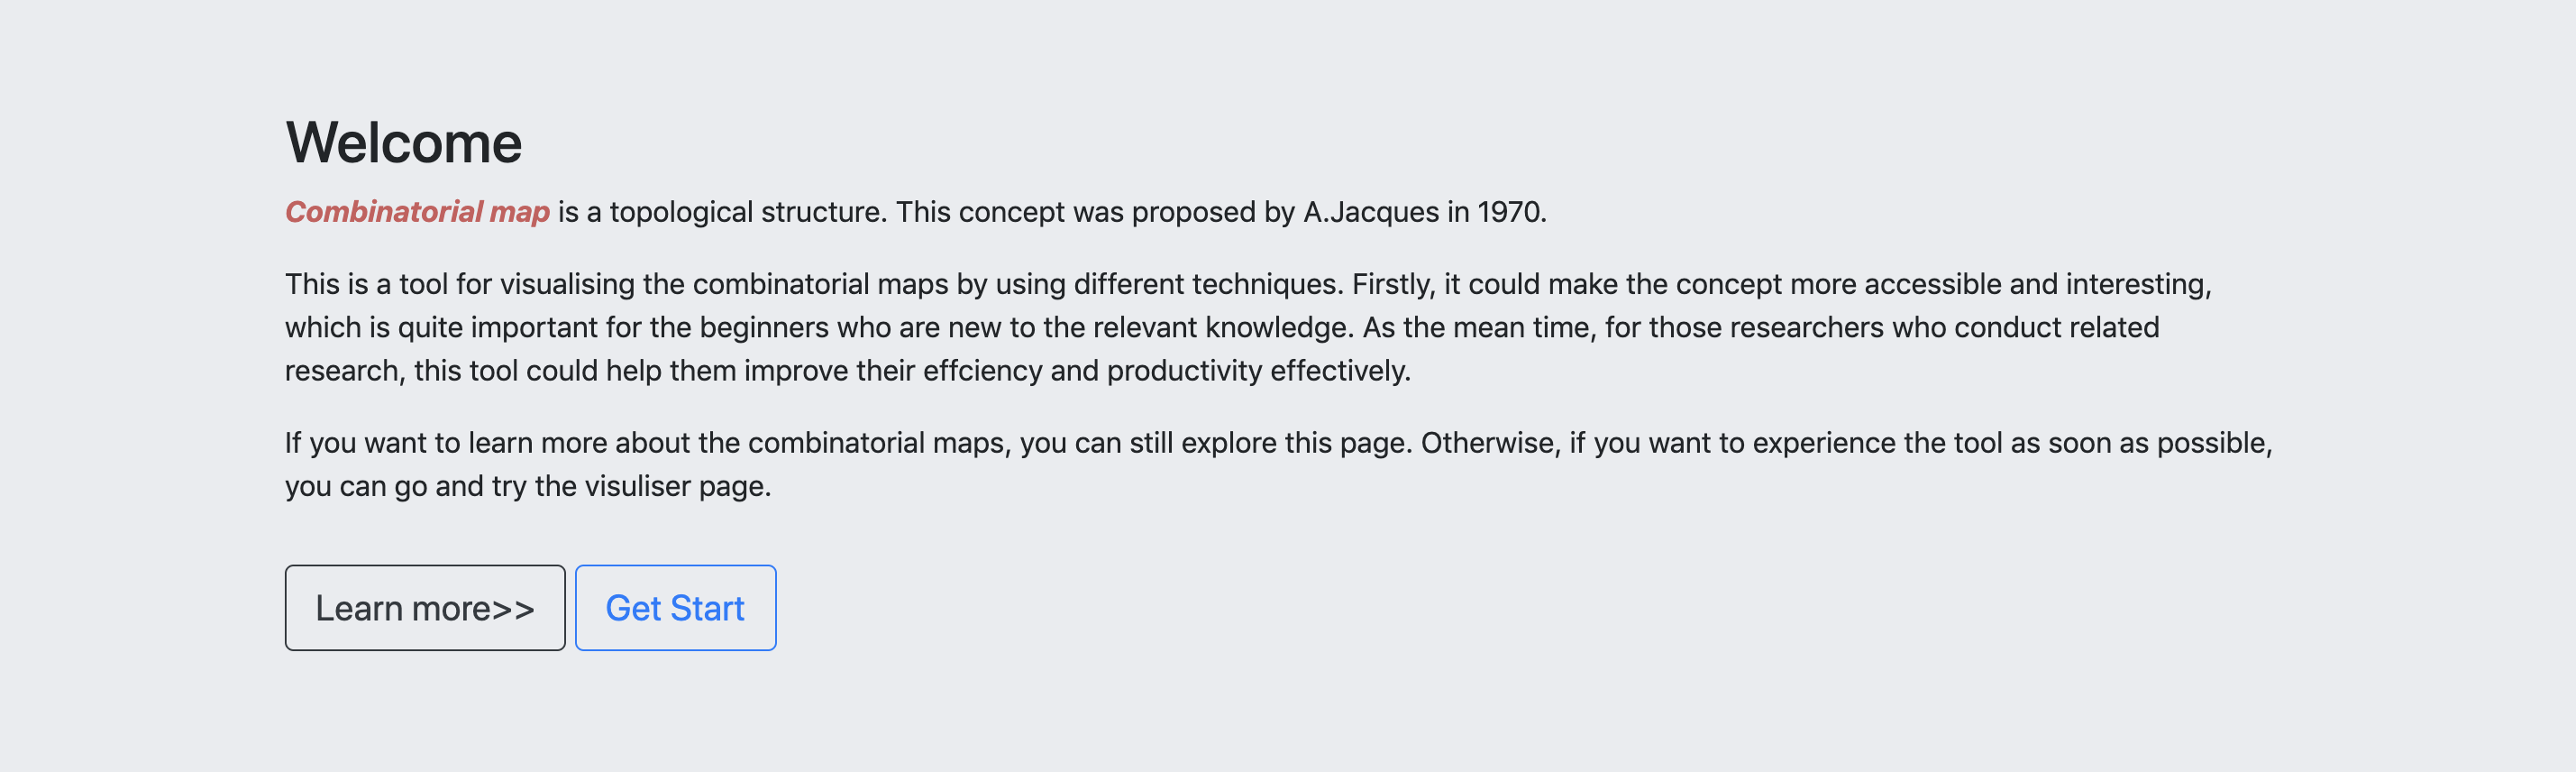
\includegraphics[width=1\textwidth]{../../image/head.png}
    \caption{The head of the introduction page.}
    \label{fig:figures:head}
  \end{figure}

  \subsubsection{Main content}
  The side bar of the main content is a table of content plugin \cite{tocplugin2019}. From the guideline of the content,  we can see that the there are three sections about combinatorial maps, visualiser and relevant algorithms. If people want to know more informations, just click the item and it will link to the specific area in the page. It can jump to the visualiser to another page when click icon beside the subtitle named visualiser.
  
  \begin{figure}[htb]
    \centering
    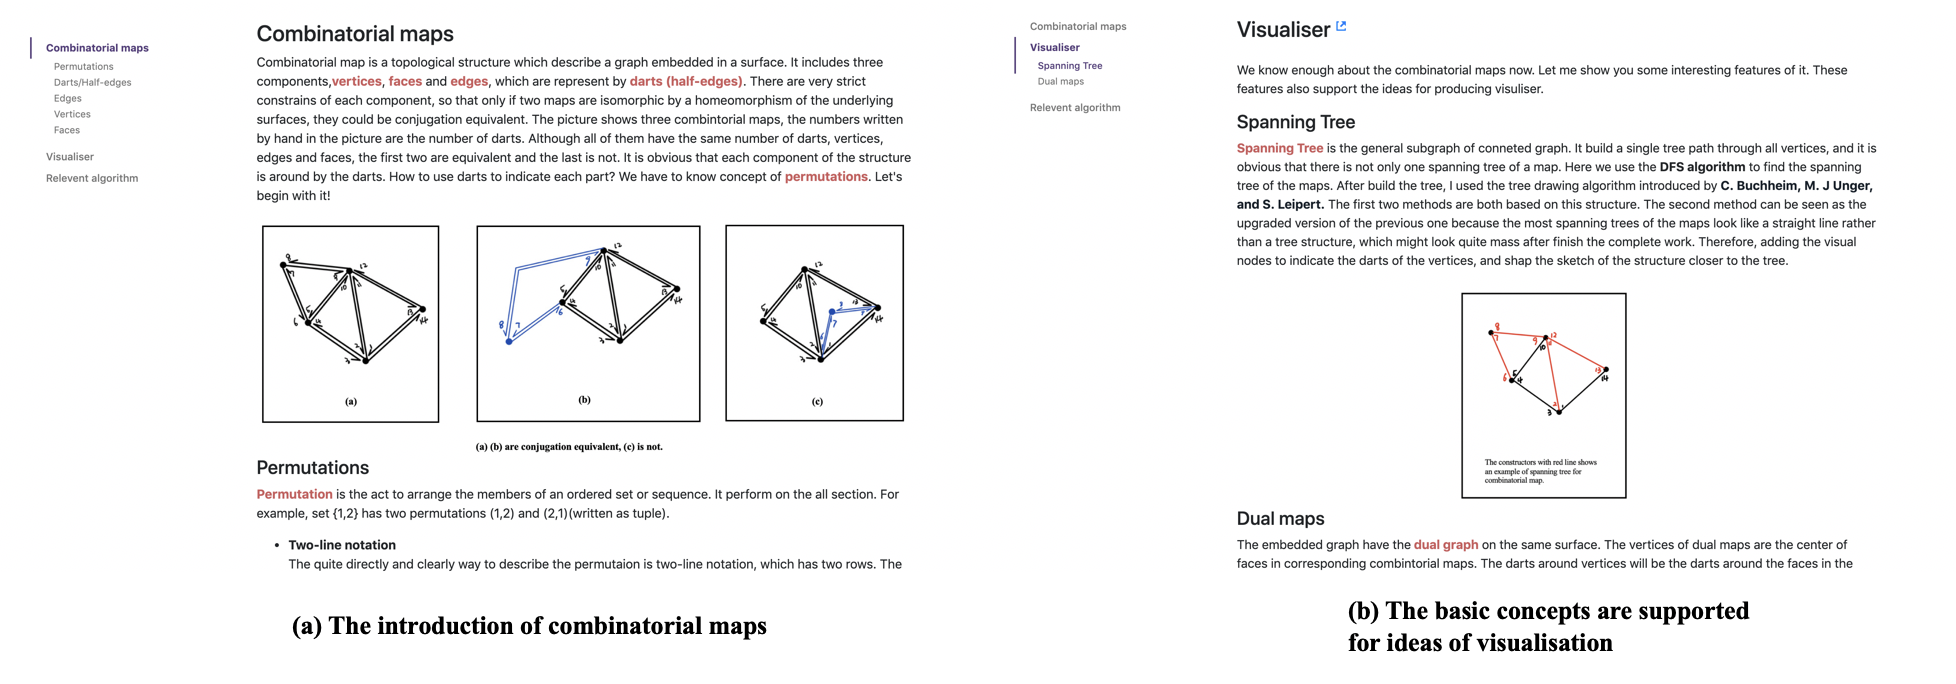
\includegraphics[width=1\textwidth]{../../image/content.png}
    \caption{The content of the introduction page.}
    \label{fig:figures:content}
  \end{figure}

  \subsection{Visualiser}
  This page plays an essential role in the whole project. It is divided into three parts, the introduction, input and output. 

  \subsubsection{Introduction}
  The page has the introduction part, as well. The introduction can help the users have a clear mind about the structure of page and know the operations and limitation of each parts. The button `learn more' means return to the introduction page to learn the knowledges of combinatorial maps and the tool. The `get start' is starting to try the visualiser.
  
  \begin{figure}[htb]
    \centering
    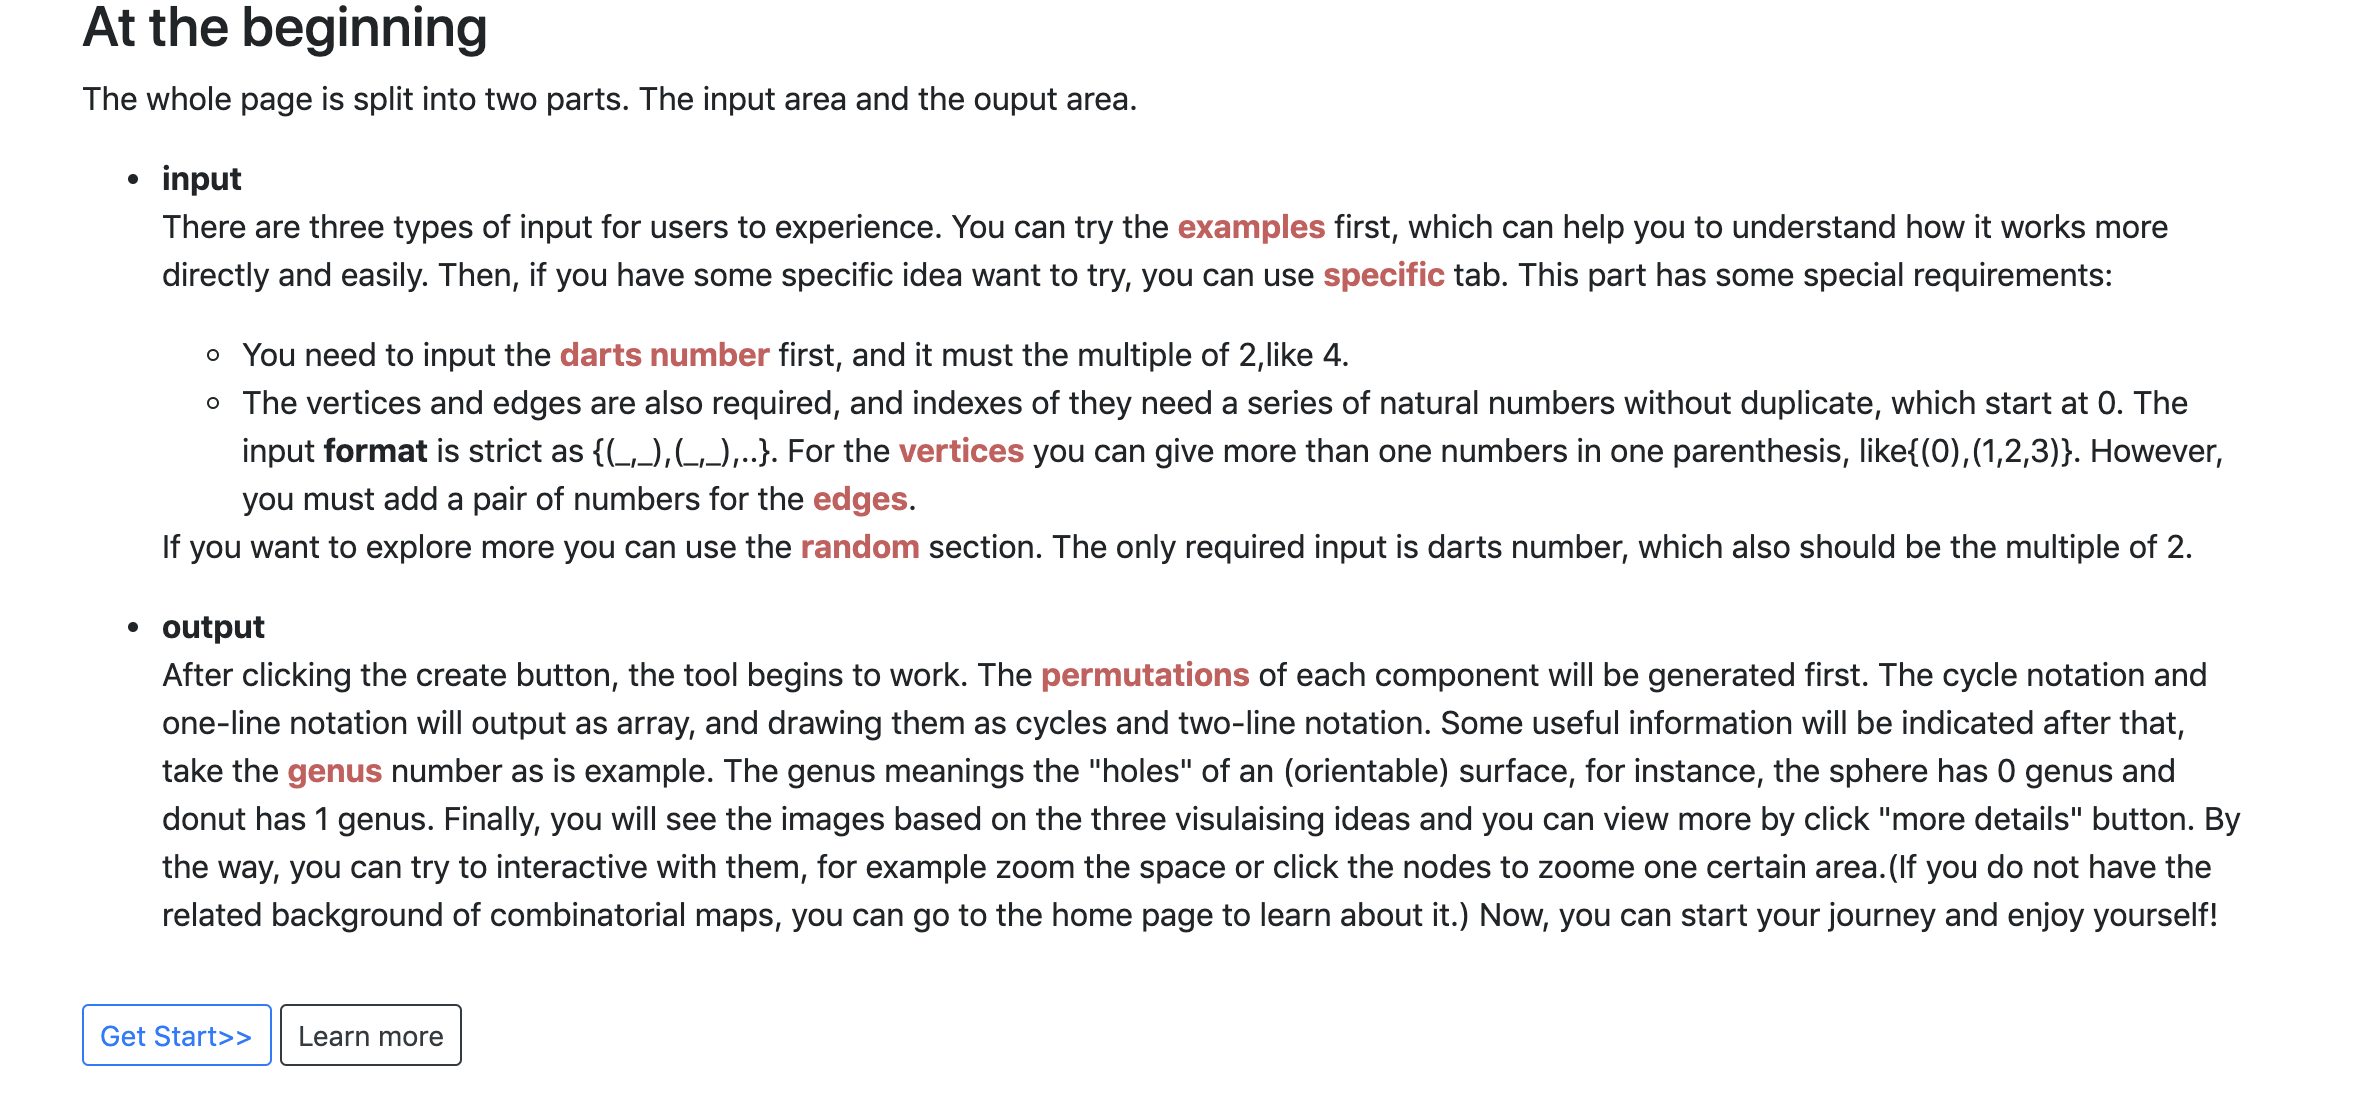
\includegraphics[width=1\textwidth]{../../image/head2.png}
    \caption{The introduction of visualiser page.}
    \label{fig:figures:head2}
  \end{figure}

  \subsubsection{Input}
  There are three type of input methods for users to choose, examples, specific and random.

  \begin{itemize}
    \item[a)] Users can select an arbitrary example as input to experience how tools work. All the examples are classical combinatorial maps including planar and non-planar maps. Click the `create’ button, the tool start to do the visualisation.
    \begin{figure}[htb]
        \centering
        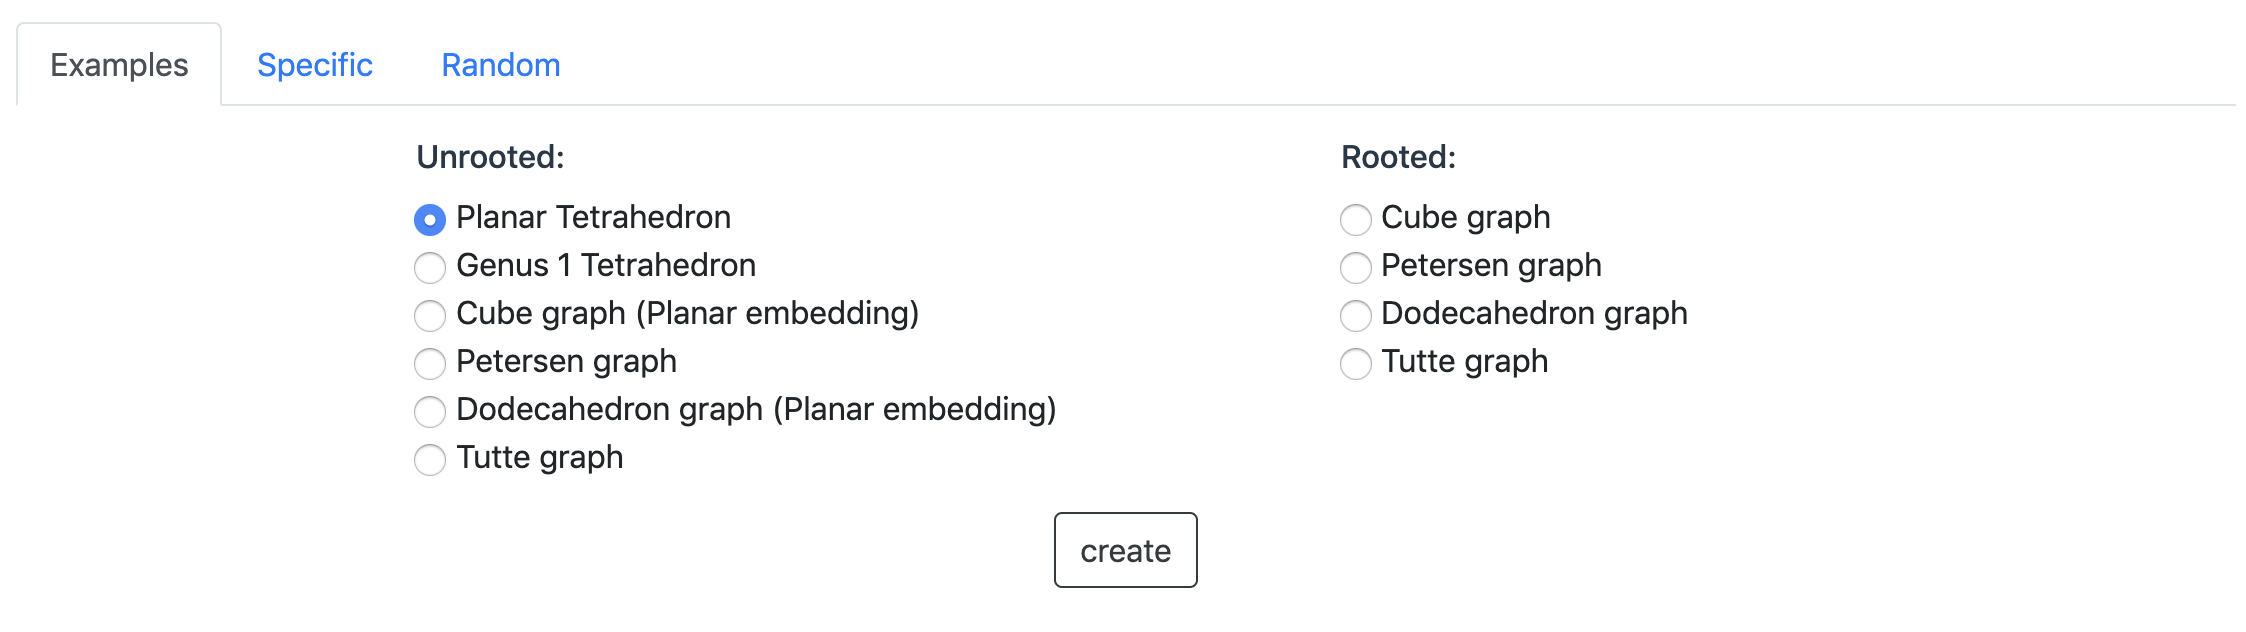
\includegraphics[width=1\textwidth]{../../image/exampletab.png}
        \caption{The examples tab}
        \label{fig:figures:exampletab}
      \end{figure}
    \newpage
    \item[b)] If users have a certain sample which is not included in the given examples, he or she can choose the  ‘specific’ tab. Three pieces of information are required, the darts number and the permutation of vertices and edges with cycle notation. The darts number should be filled at first and correct,otherwise, users cannot continue doing other operations.
    \begin{figure}[htb]
        \centering
        
\includegraphics[width=1\textwidth]{../../image/specifictab.png}
        \caption{The specific tab}
        \label{fig:figures:specifictab}
      \end{figure}

    Some conditions are used to validate whether the input is correct or not. A JAVASCRIPT library called Vue.js\cite{you2018vue} is used to do the real-time validation and data communication.  Firstly, for the darts number, it must be a number that is multiple of 2. Secondly, the permutation of vertices and edges have their own format the users should obey, for example, the numbers of each permutation must be a series of natural number start from 0 and the largest number must be the darts number minus 1. For the vertices, the numbers of elements in the parentheses must more than 1, while, in edges permutation, it can only have two numbers. These constraints provide a structural clue to parse the inputs whose data type is string. For parsing the string to a readable and operational data type, a regular expression is used, for instances, the expression ‘/\^{}\textbackslash\{(\textbackslash([0-9]+(,[0-9]+)\textbackslash))(,\textbackslash([0-9]+(,[0-9]+)\textbackslash))*\}\$/’ matches the format of inputted edges. The real-time validation will check the input at every time when users change the content. If the wrong input, the system will promote the users with an error massage and provide a right examples. The users can also click the `?’ button to check the requirement of the inputs.
    \begin{figure}[htb]
        \centering
        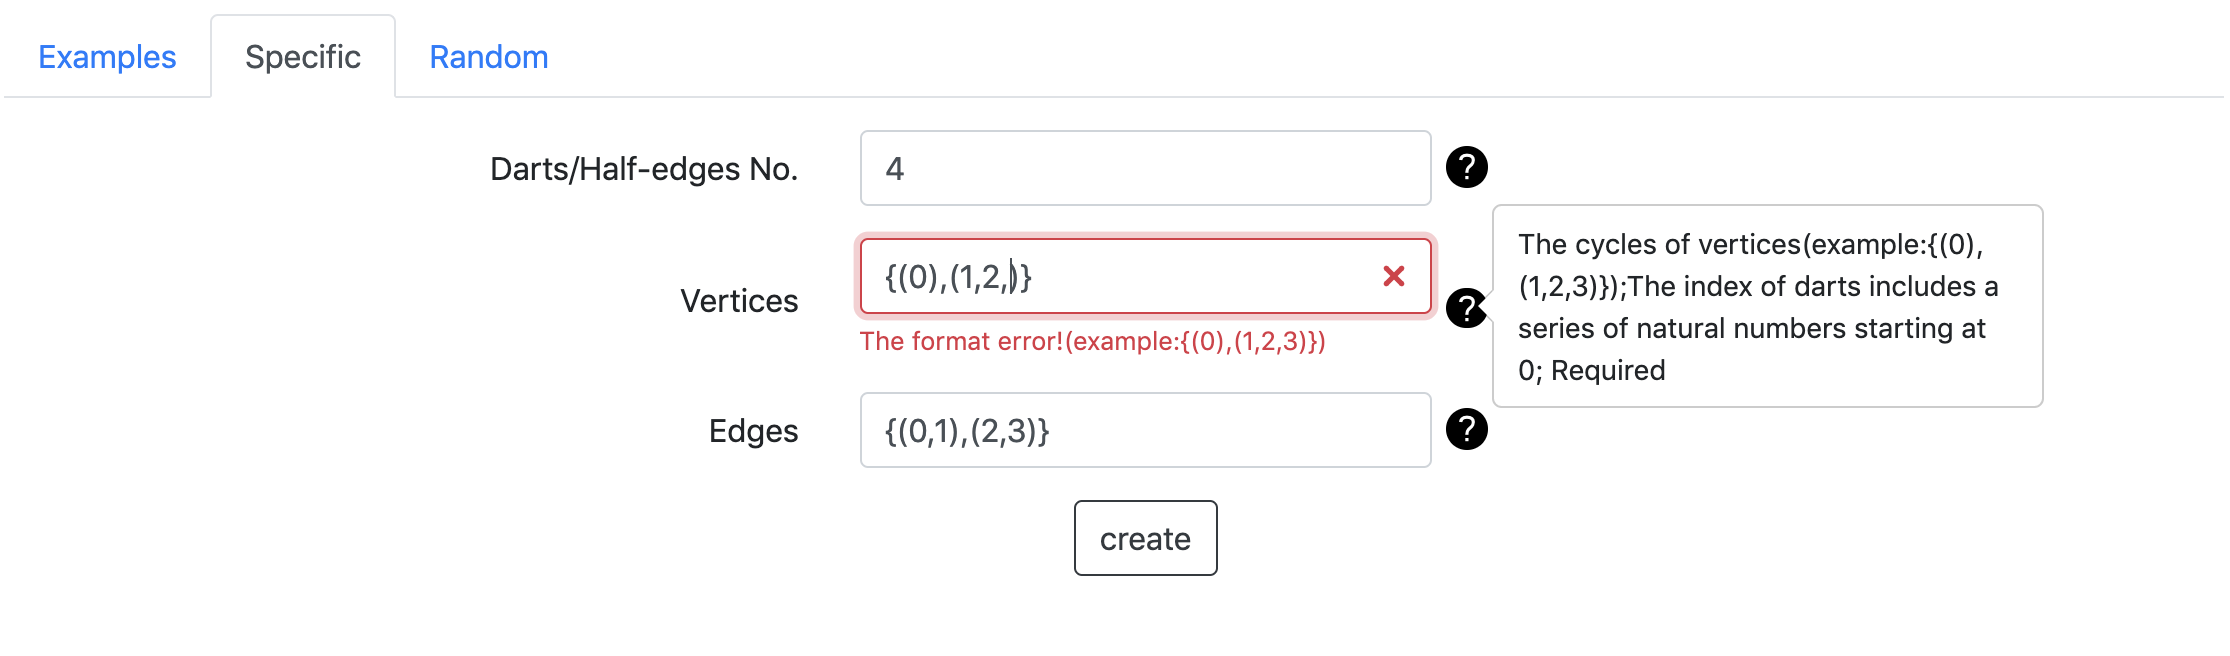
\includegraphics[width=1\textwidth]{../../image/errorinput.png}
        \caption{The error massage and notes.}
        \label{fig:figures:errorinput}
      \end{figure}
    
    \newpage
    \item[c)] The last tab is for users who do not have a specific example of combinatorial maps or those who just want to seek various results of maps with the same darts number, hence the darts number is required. Meanwhile, users can decide whether needs to limit the number of vertices for the map and the number must not more than darts number.
    \begin{figure}[htb]
        \centering
        
\includegraphics[width=1\textwidth]{../../image/randomtab.png}
        \caption{The random tab}
        \label{fig:figures:randomtab}
      \end{figure} 
      
    Regardless of whether the user has entered the number of vertices, the entire process starts with generating a random permutation of edges \textit{genRandomEdges()}: 1.Defining a set of darts \(D\); 2. Choosing arbitrary two members of it and delete them; 3. Pushing selections as array into the edges array \(EC\); 4.Repeating 2 and 3 steps until \(D\) is empty. 

    Creating the permutation of vertices is the next step, which depends on whether the users enter the number of vertices. If the input is empty, using Fisher-Yates shuffle algorithm \cite{fisher1943statistical} to generate a vertices permutation with one-line notation \textit{genRandomVerticesPerm()}. The logic of the function is as below: 1. Declaring a set \(VP\) whose length is the number of darts \(n_d\) and the elements follow the natural order; 2.For each member whose index is \(i\), selecting a random number \(j\) from 0 to \(n_d -1\); 3. Swapping the elements \(VP[i]\) and \(VP[j]\). 
    
    Another function \textit{genRandomVerticesByNum()} is used when the input is not empty as \(n_c\).  At the beginning, defining a set \(VC\) which has \(n_c\) members of empty array. The core of the function is a loop with period \(n_d\). For each time \(n\), randomly choosing a number \(r_d\) between 0 and \(n_c -1\). Adding \(n\) to the array \(VC[r_d]\). Redefining \(VC\) if any of the element is still empty. Actually the random function the JAVASCRIPT defined is useless and unfair, thus, a new random generator is defined. Even though, it still need to verify that whether the \(VC\) contains the empty elements.

    The function \textit{convertToPermutations()} aims to convert the cycle notation to one-line notation and \textit{convertToCycles()} inverses the process. Finally, using the function \textit{isConnection()} mentioned above validates the whether the map is connected. If it is not connected, restarting from the first step or continuing to the next step when it is connected.
    \begin{figure}[htb]
        \centering
        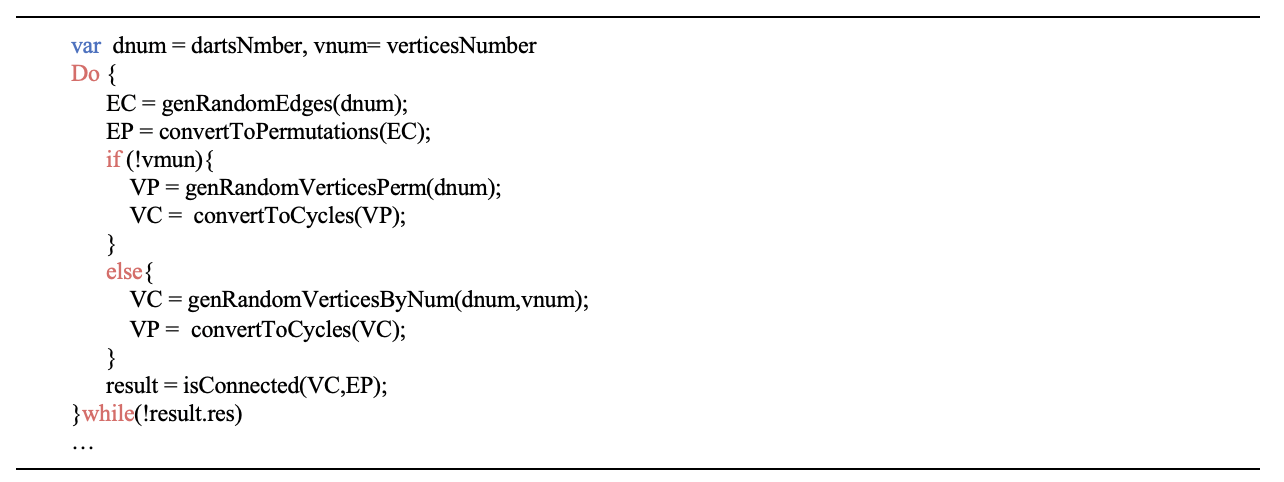
\includegraphics[width=1\textwidth]{../../image/randompro.png}
        \caption{The construct of generating a random combinatorial map with the JAVASCRIPT implementation.}
        \label{fig:figures:randompro}
      \end{figure} 
  \end{itemize}

  \subsubsection{Output}
  The output includes describing and visualising each component, displaying other information and showing the results of the approaches.
  \begin{itemize}
    \item[a)] Components of a combinatorial map. It is known that the permutation is used to indicate the permutations. In order to supporting more specific details, every notations of permutations have been visualised. The \cref{fig:figures:components} shows the results of each components, the nodes are the darts. The different colours can distinguish the components easily. It is difficult to identify the minutiae of the nodes and edges and zooming the space by click the nodes or other ways can solve the problem. The icon at the end of permutations is to reset the canvas.
    \begin{figure}[htb]
        \centering
        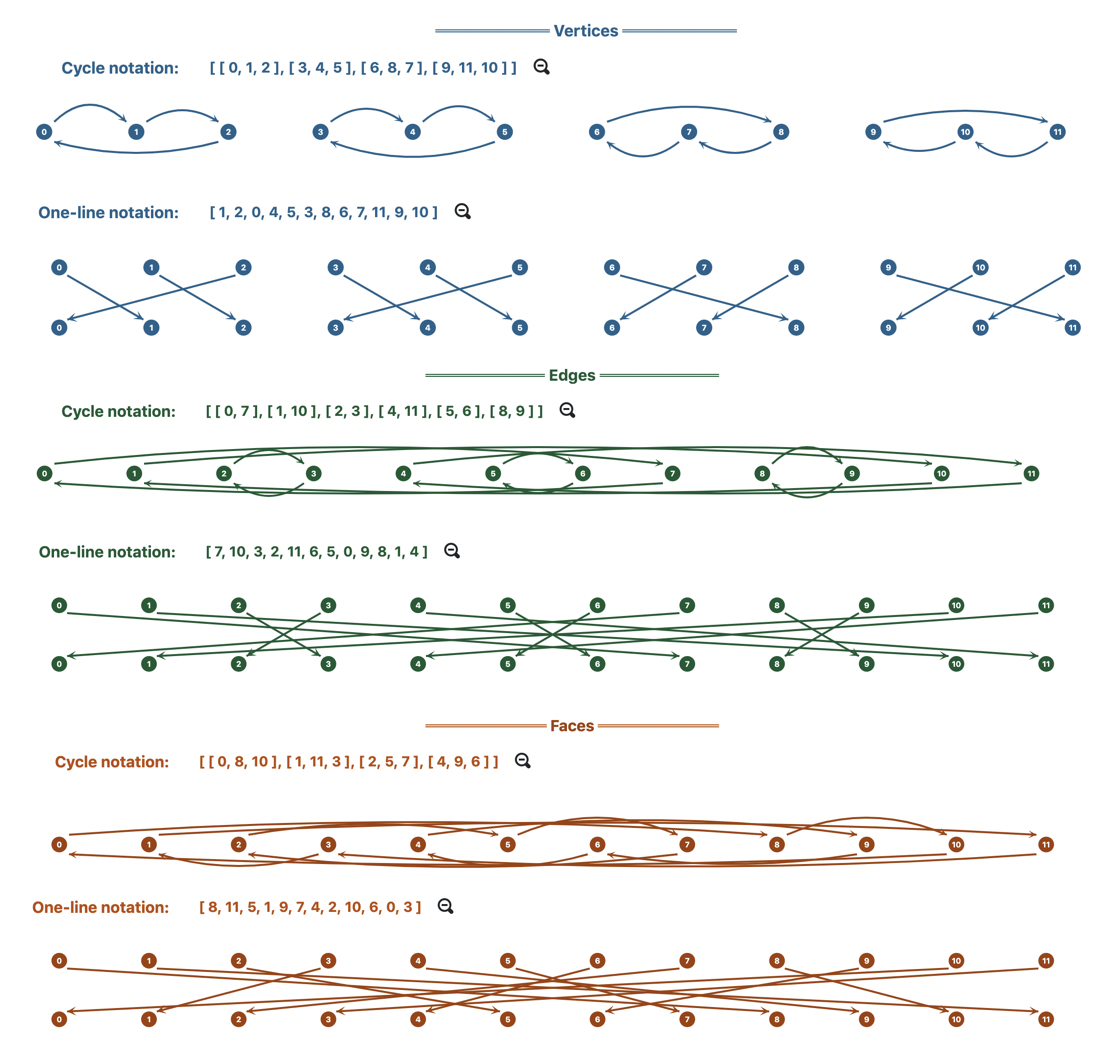
\includegraphics[width=1\textwidth]{../../image/components.png}
        \caption{Visualisation of each component}
        \label{fig:figures:components}
      \end{figure}
    \newpage
    \item[b)] Four characters faces number, vertices number, darts number and genus number are supplied in the `other characters’ area.
    \begin{figure}[htb]
        \centering
        
\includegraphics[width=1\textwidth]{../../image/otherinfor.png}
        \caption{Other information}
        \label{fig:figures:otherinfor}
      \end{figure} 
    \item[c)] The bottom of the page is the results of approaches. Every results show as PNG format, and hover effect cover on the images tell the idea of the methods. If users want to see the details, clicking the `MORE DETAILS’ button and an interface will pop out. A real SVG image displays on the interface and the necessary information is wrote at the side of it.
    \begin{figure}[htb]
        \centering
        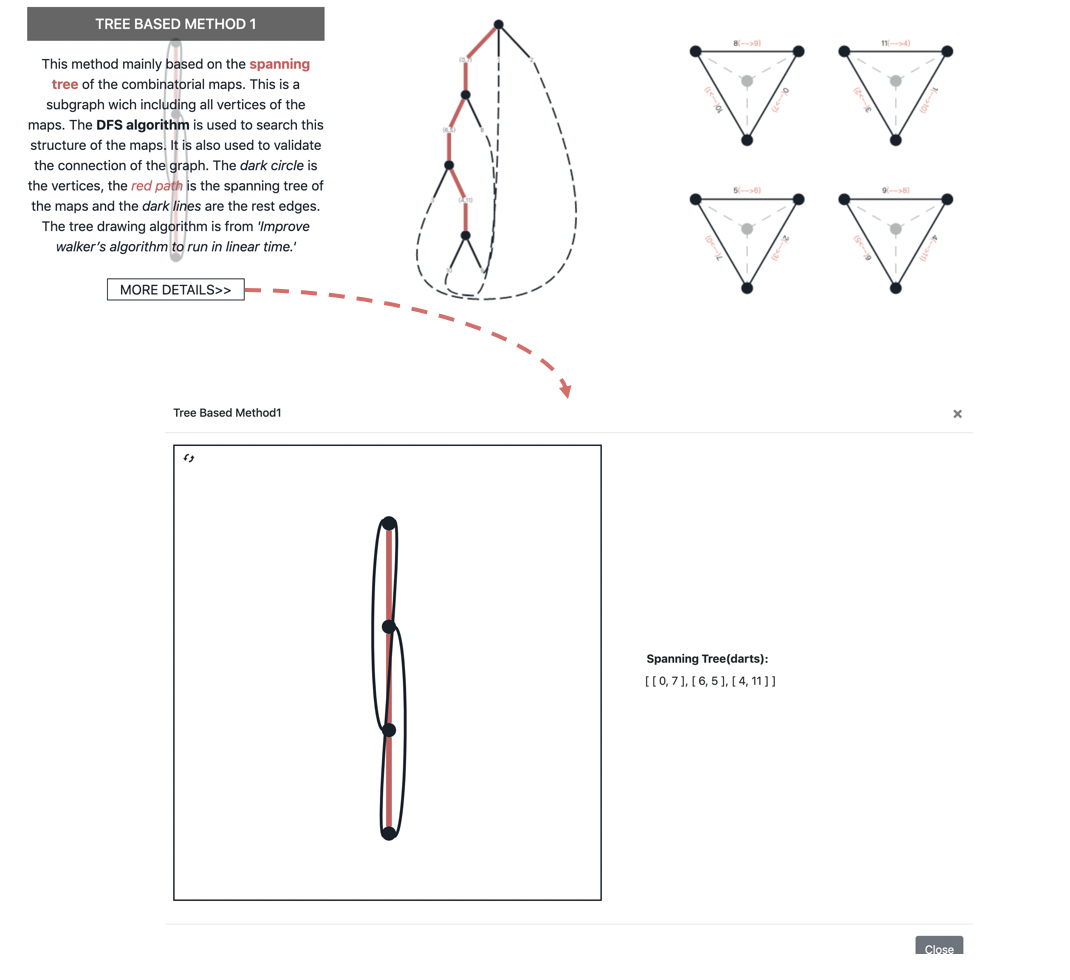
\includegraphics[width=1\textwidth]{../../image/resultsofmethod.png}
        \caption{Results of methods}
        \label{fig:figures:resultsofmethod}
      \end{figure} 
  \end{itemize}

 
% !TeX encoding=utf8
% !TeX spellcheck = en-US

\chapter{Evaluation}

\section{Testing the visualisation method}

The visualising methods is the main work of the project, thus, comparing each method and discovering the problems of the methods are important.

\subsection{Cross in planar map}
The most essential feature of planar graph is no cross inside of the graph. Therefore, this is the primary assessment criterion for the methods when generate a planar map.

\begin{figure}[htb]
    \centering
    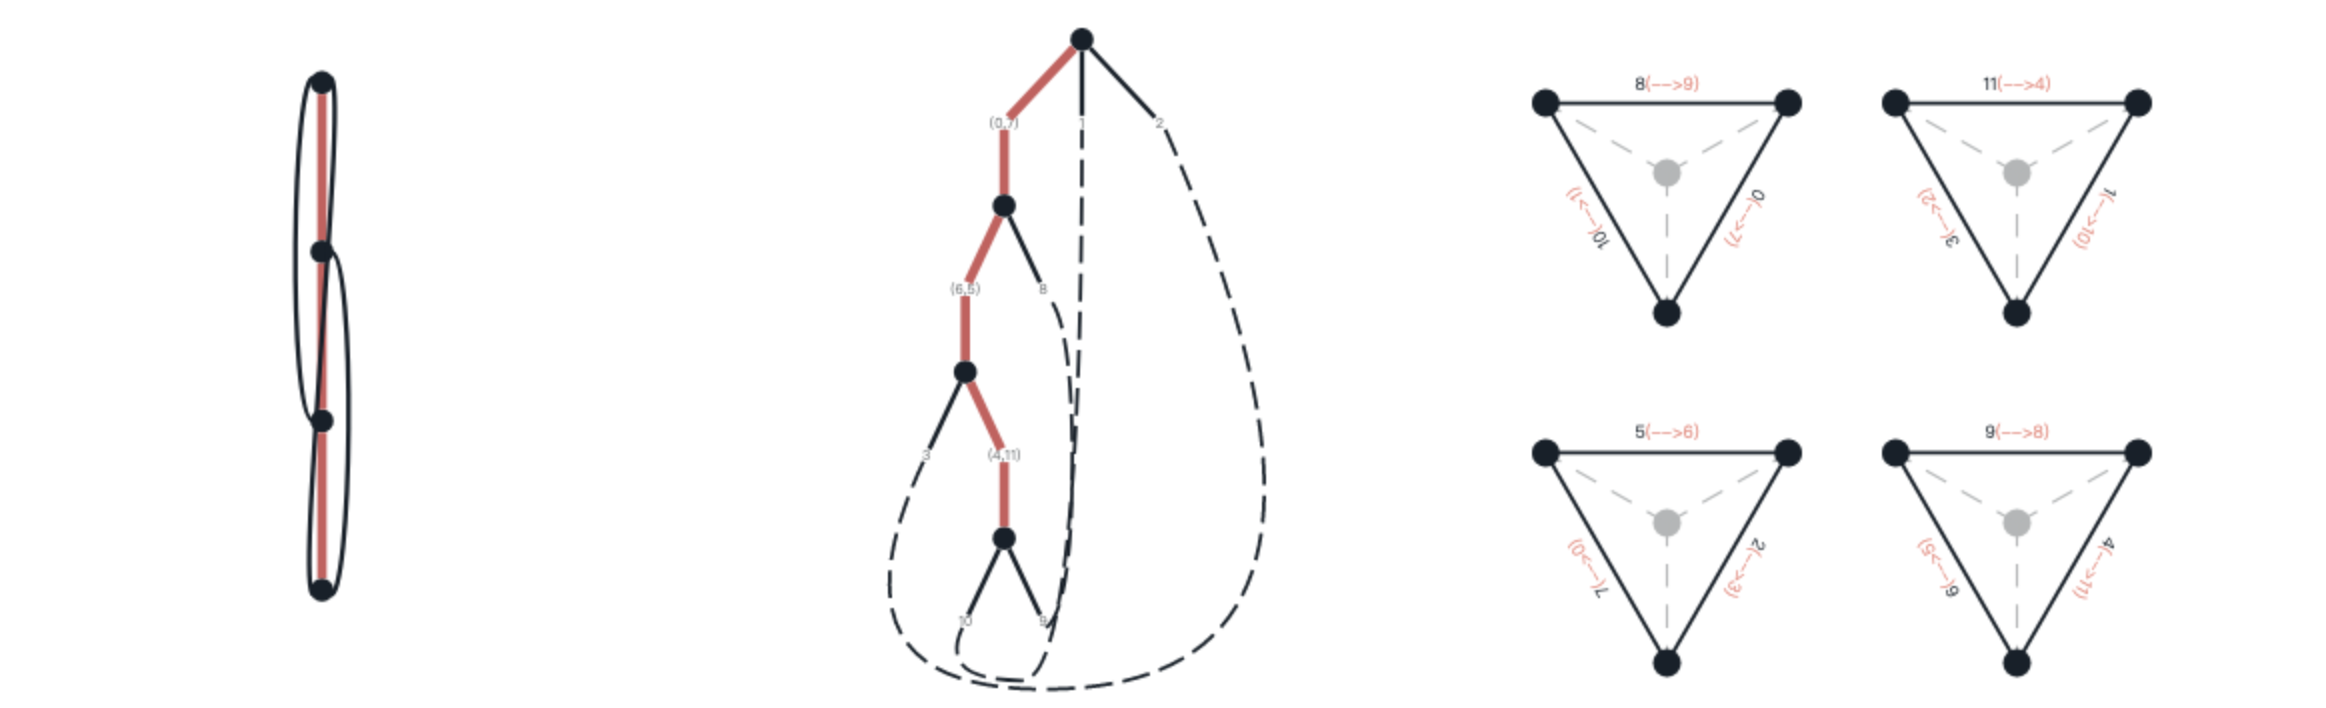
\includegraphics[width=0.8\textwidth]{../../image/cross1.png}
    \caption{Results of planar Tetrahedron.}
    \label{fig:figures:cross1}
  \end{figure}

  The \cref{fig:figures:cross1} shows a simple planar map called planar Tetrahedron, it is obvious that the last two methods work well and avoiding the cross successfully, though the gap between lines in the second method is too narrow. However, the first approach cannot handle the problem completely.

  \begin{figure}[htb]
    \centering
    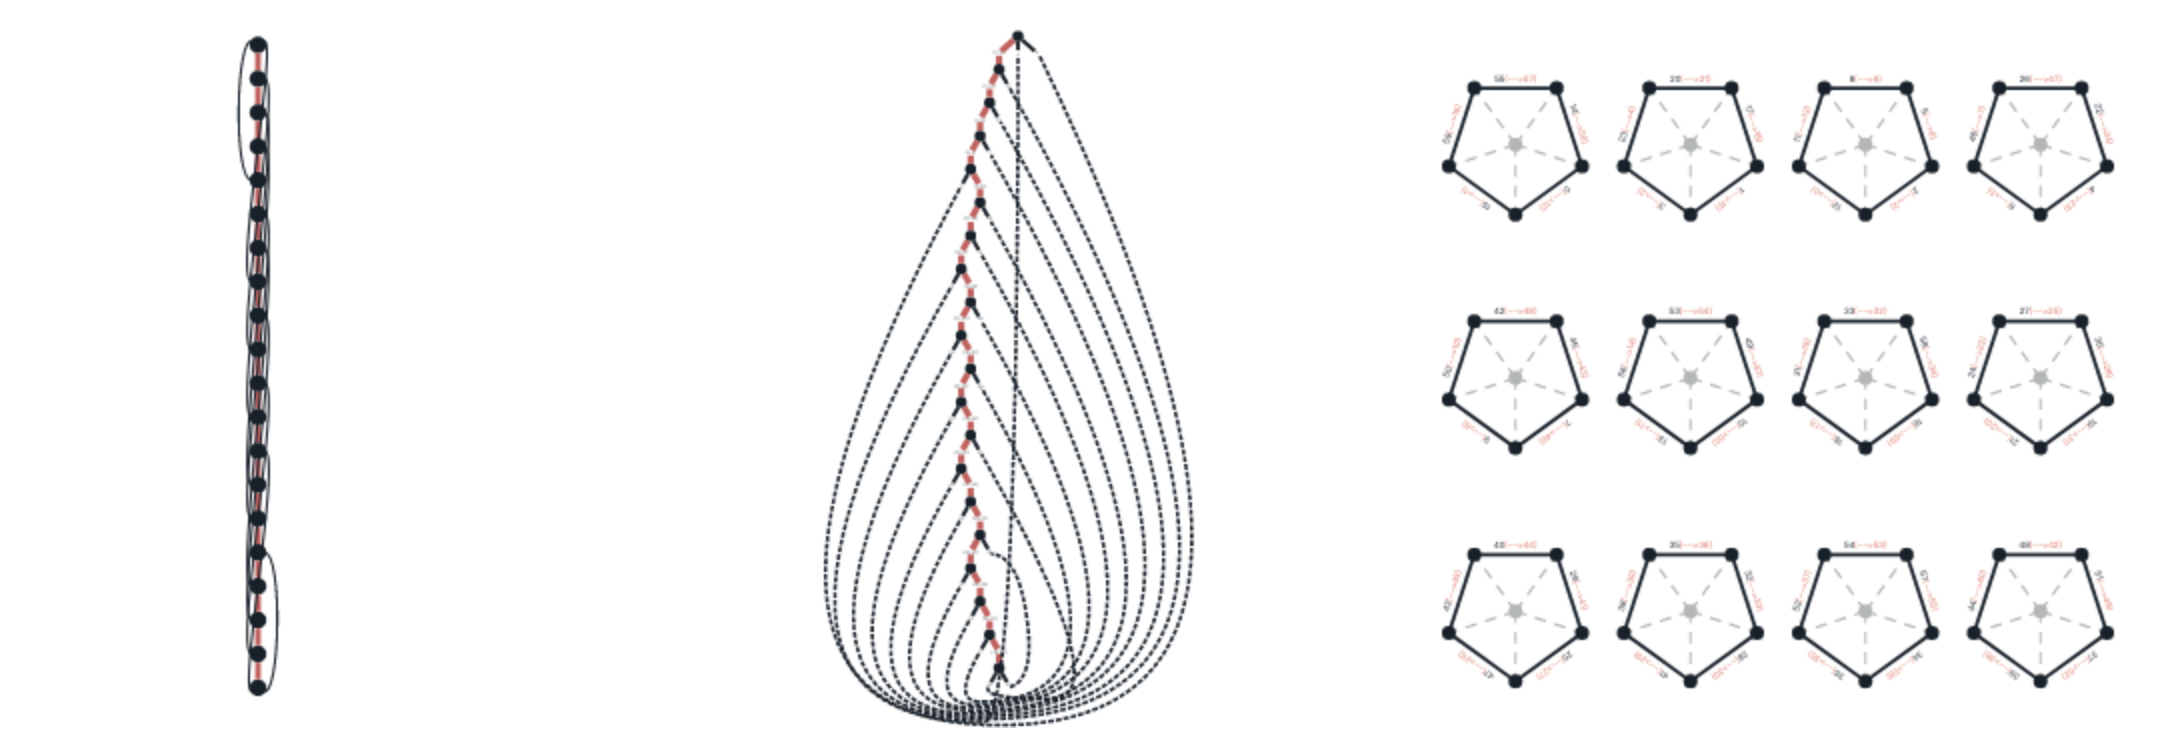
\includegraphics[width=0.8\textwidth]{../../image/cross2.png}
    \caption{Results of dodecahedron graph.}
    \label{fig:figures:cross2}
  \end{figure}
  The solutions of a larger map for dodecahedron graph display in the \cref{fig:figures:cross2}. For this map, the first map becomes mass and unclear, and the last method is still tidy without cross. The second method, however, is not up to standard because the cross appear in the two of curves.
  \begin{figure}[htb]
    \centering
    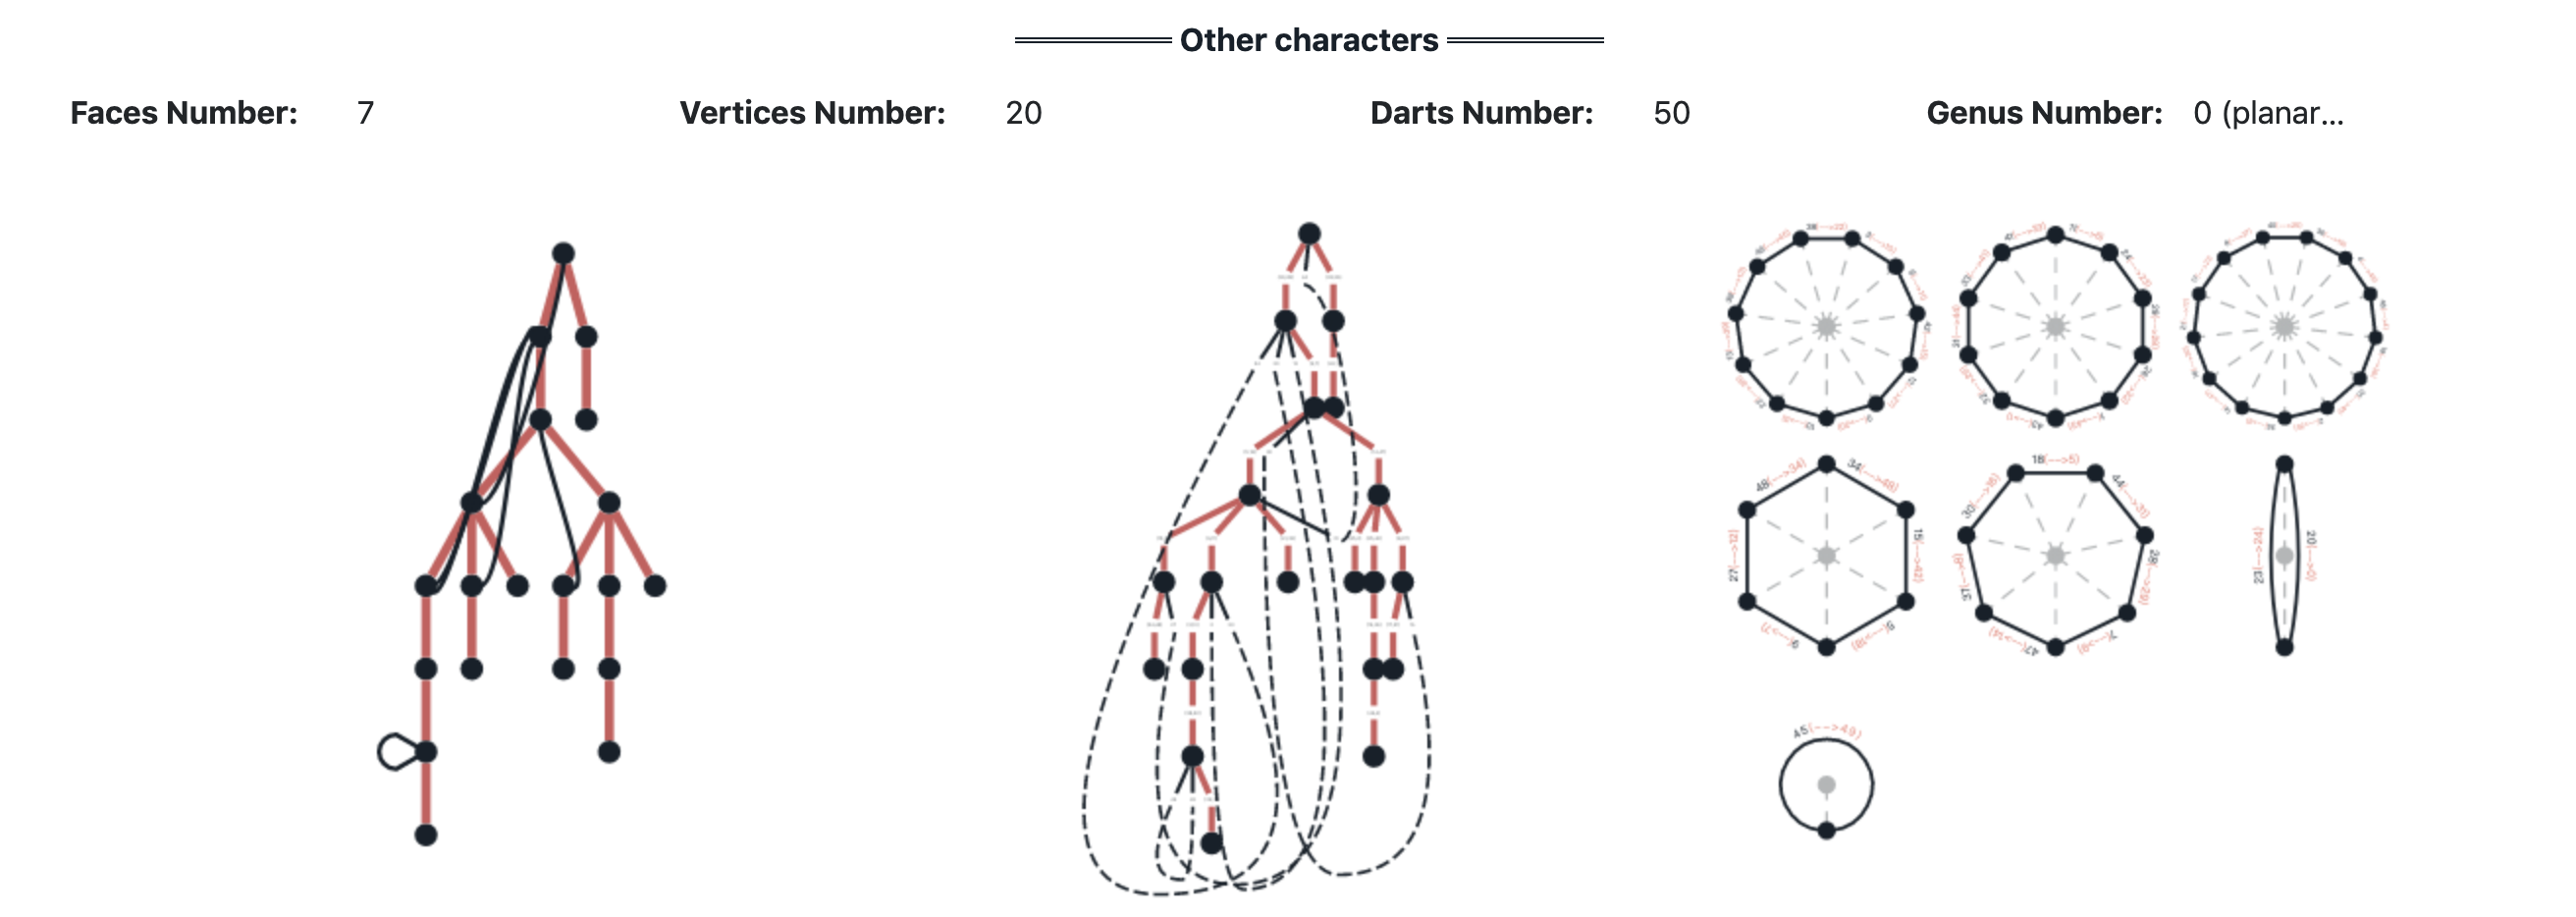
\includegraphics[width=0.8\textwidth]{../../image/randomplanar.png}
    \caption{Results of a random planar map.}
    \label{fig:figures:randomplanar}
  \end{figure}
  \newpage
  Besides the example, the \cref{fig:figures:randomplanar} gives results of a random planar maps. The darts number of the map is 50. The vertices number is fixed to produce a planar map with high probability. The genus number is 0, thus this is a planar map. After observing the results, the result is the same with the last example that the cross occurs in the first two results but not exists in last one.

  \subsection{Time consumption}
  The time consumption is a condition to estimate whether a method or an algorithm is better for a certain problem. 

  \begin{figure}[htb]
    \centering
    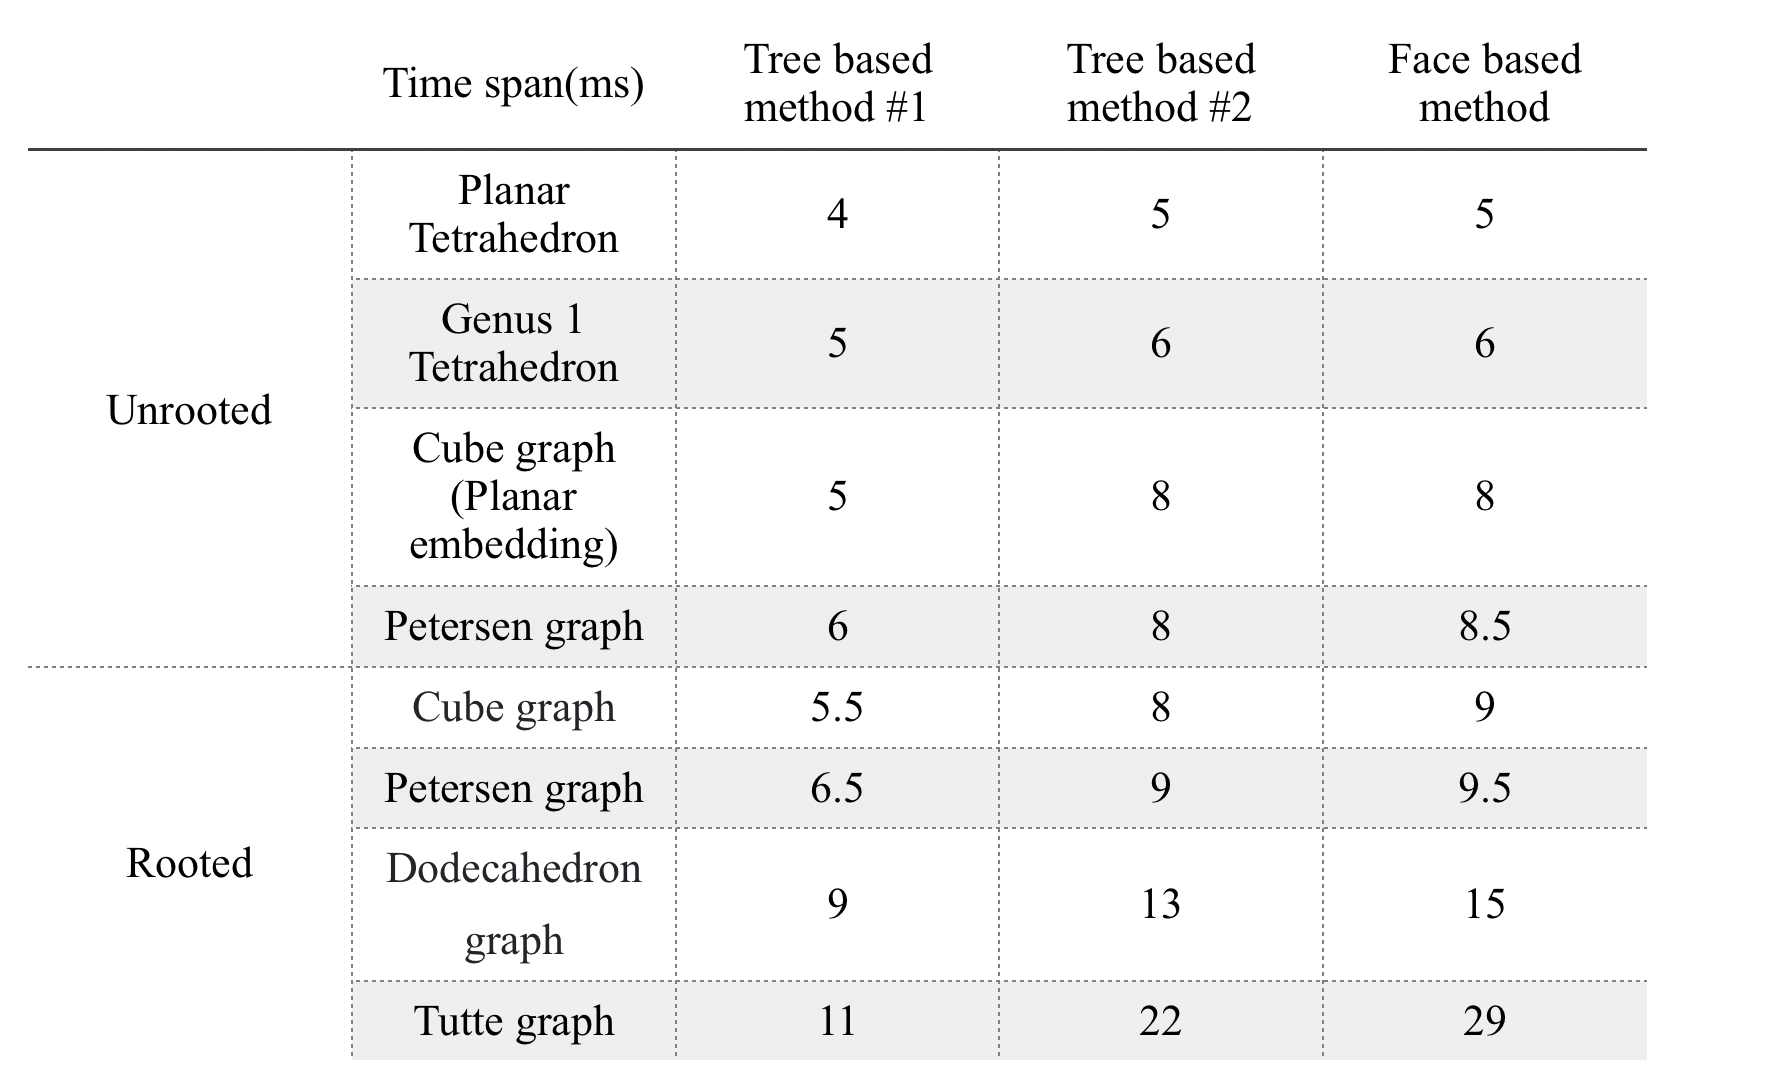
\includegraphics[width=1\textwidth]{../../image/timeconsume.png}
    \caption{The time consuming of the methods for different maps.}
    \label{fig:figures:timeconsume}
  \end{figure}
  We just test this features of each approach on the examples, cause the time for the same method might be a little different for each running. In order to maintain the accuracy of the results, the consequence comes from the average of 10 times testing with the same map. From the result, first tree based method use the least time.  The time span of the improved tree based method and the faces based method almost the same, but the later method spends more time.

  \subsection{Clarity}
  The requirement of the clarity for a visualising result is that users can analysis the output directly and the edges should not be cramped together and have an explicit identity. Firstly, trying a simple combinatorial map whose darts number is 8. Every drawing results of the map is tidy and transparent.
  \begin{figure}[htb]
    \centering
    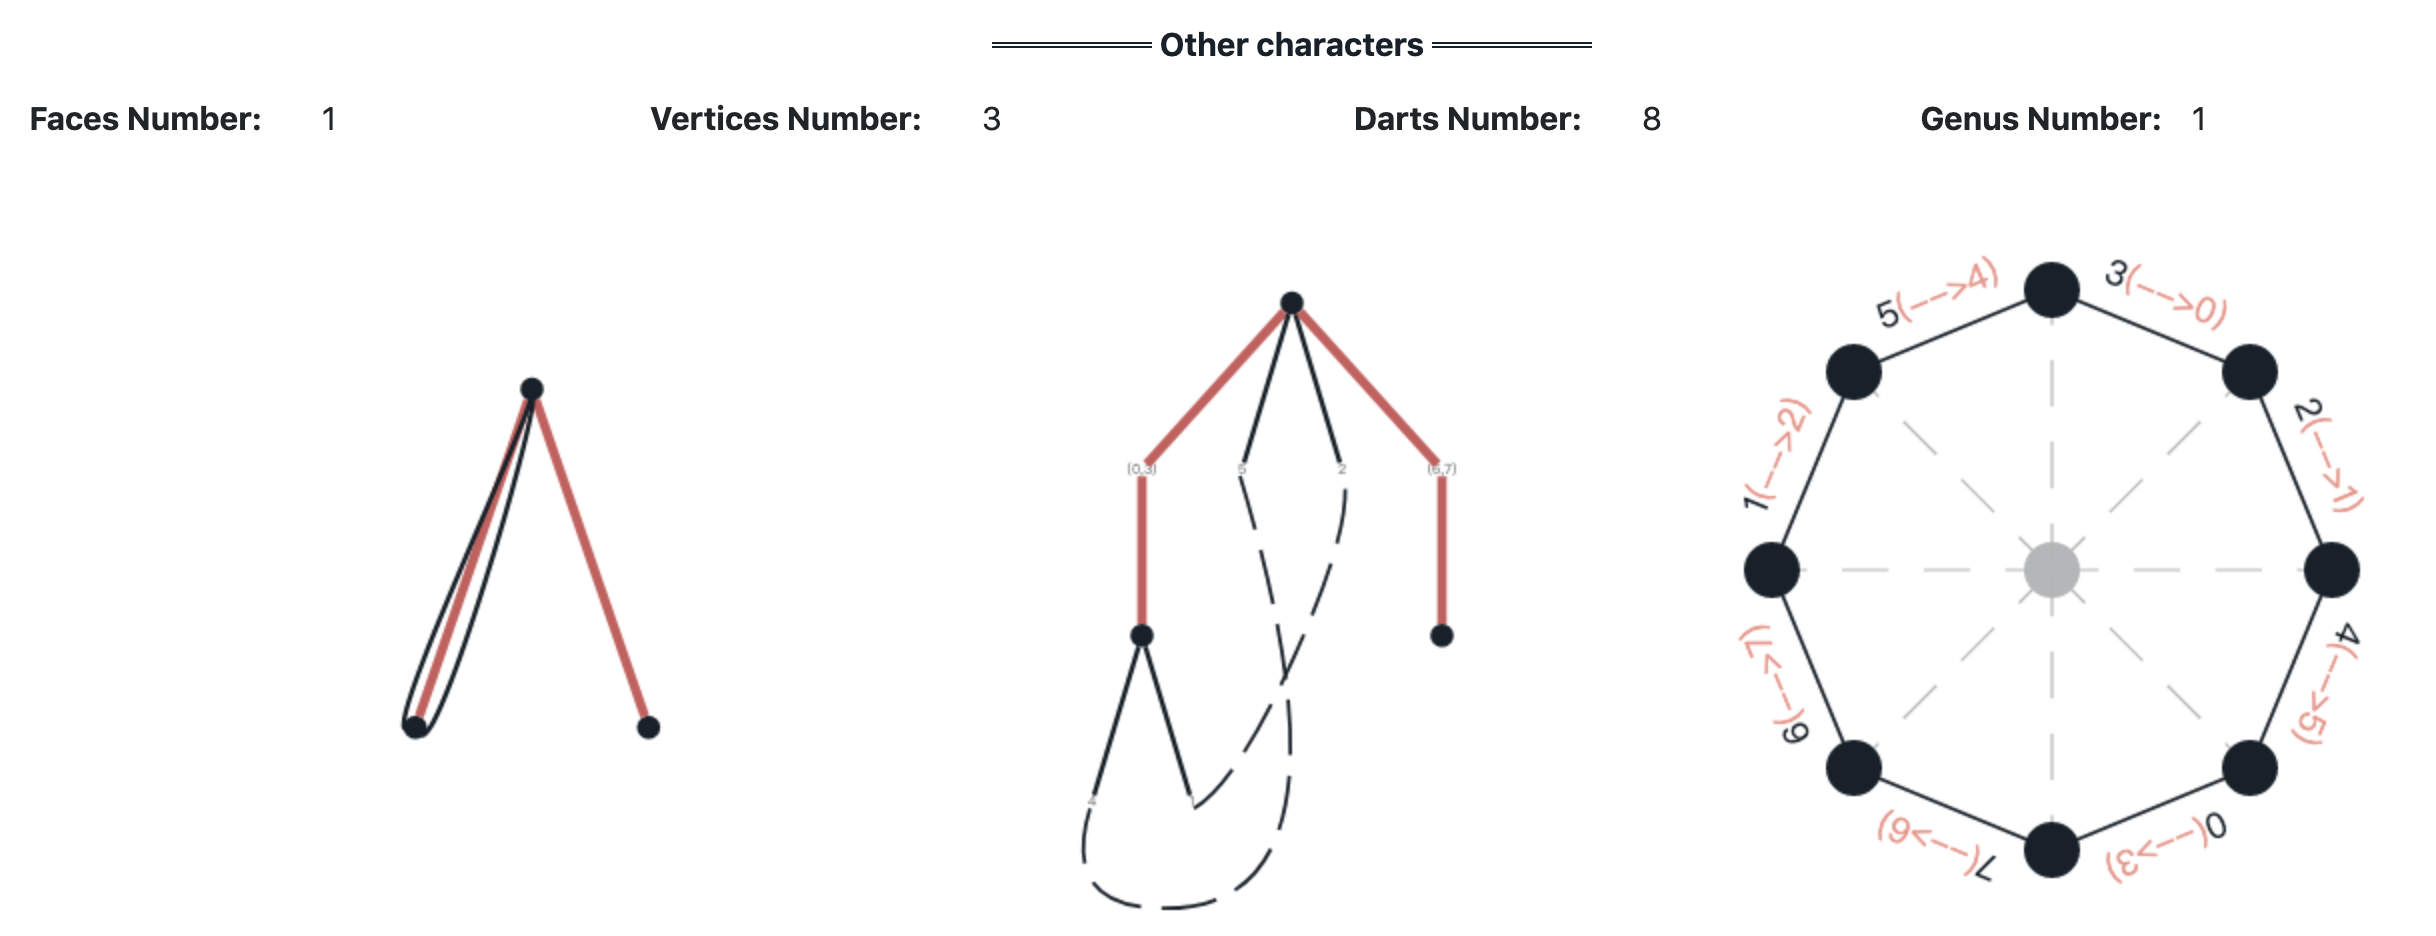
\includegraphics[width=1\textwidth]{../../image/clear1.png}
    \caption{A random map with 8 darts.}
    \label{fig:figures:clear1}
  \end{figure}

  Drawing a larger combinatorial maps based on the 100 darts. The edges cramped together and hardly to recognise the structure of the map for the first method. The second method still retain a beautiful and complete structure. The most neat result is the last one.

  \begin{figure}[htb]
    \centering
    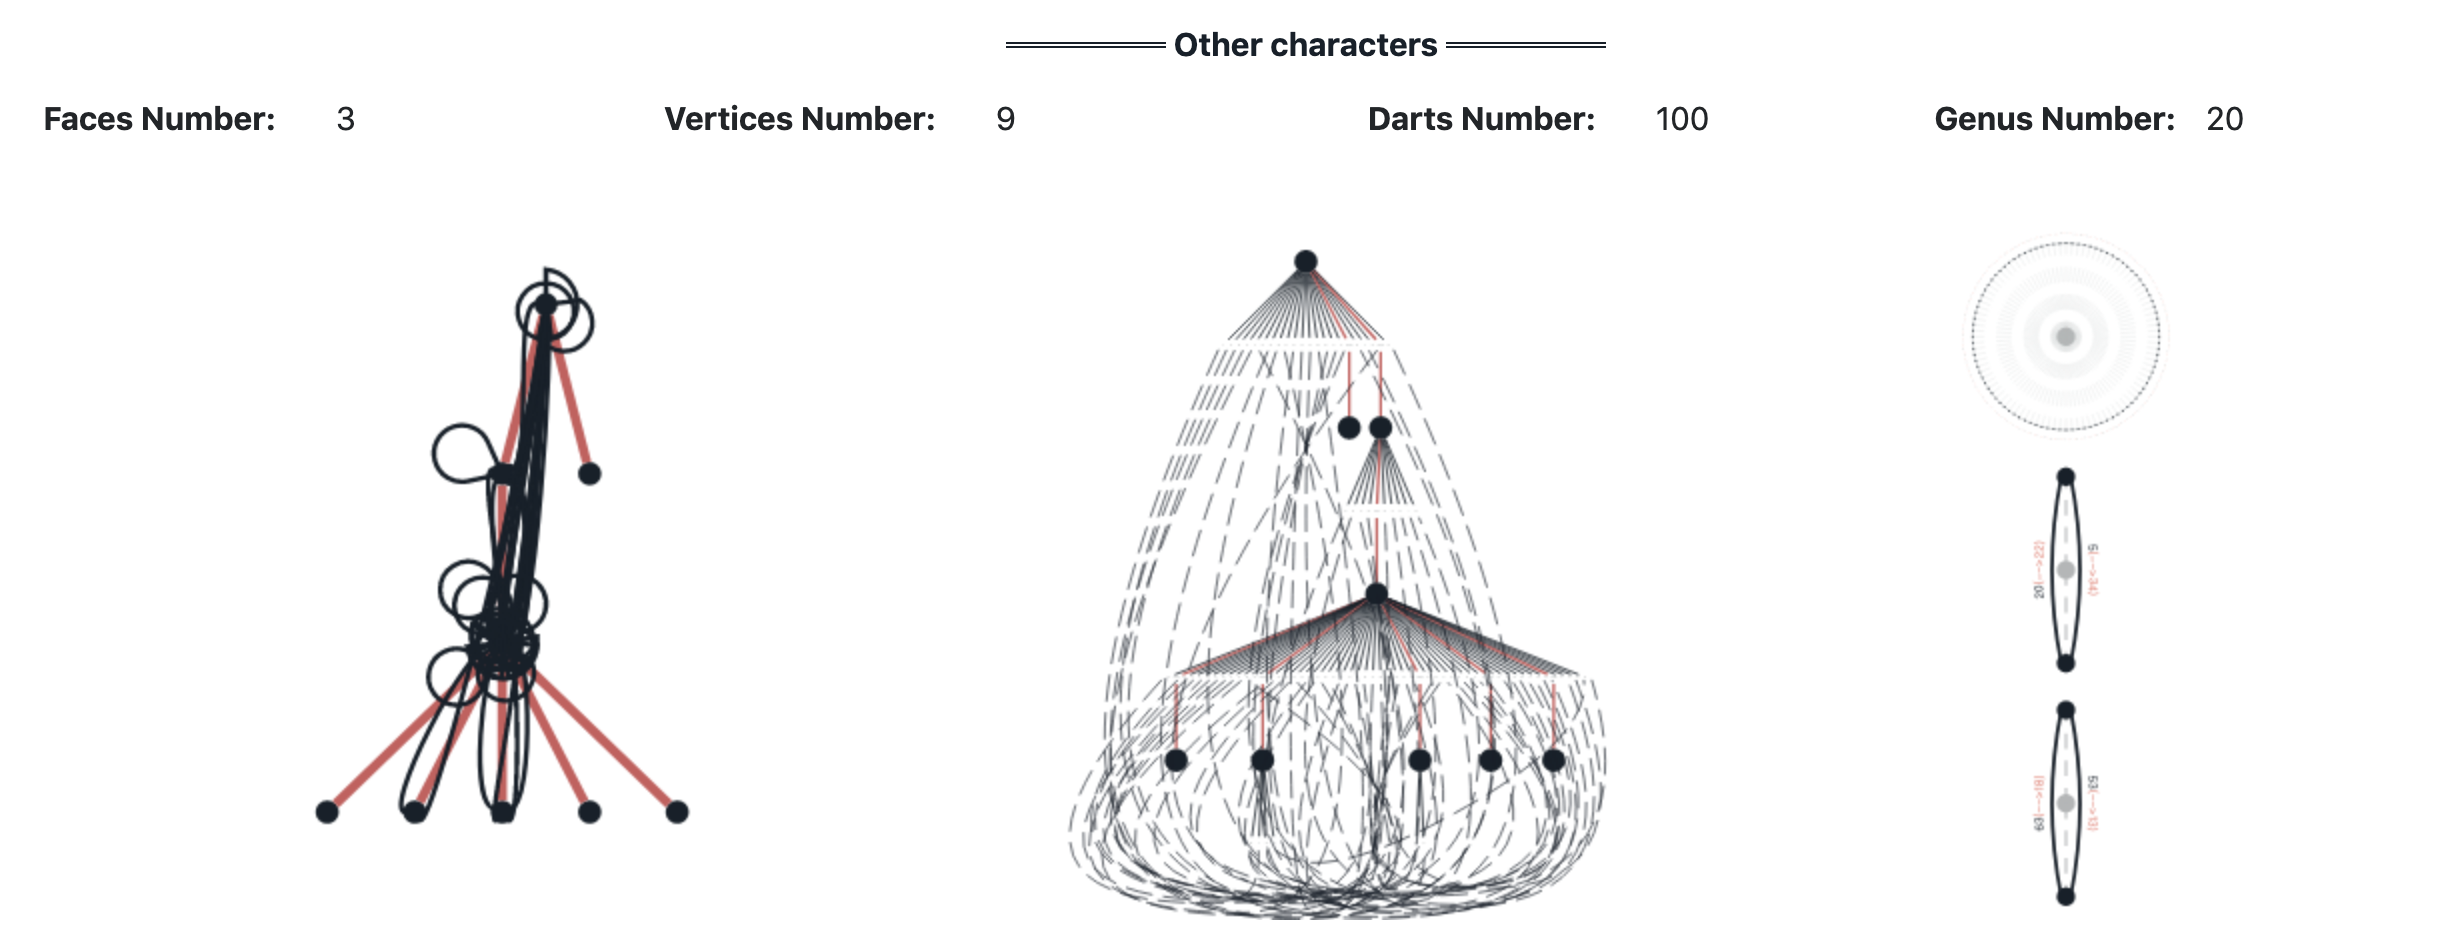
\includegraphics[width=1\textwidth]{../../image/clear2.png}
    \caption{A random map with 100 darts.}
    \label{fig:figures:clear2}
  \end{figure}

  The \cref{fig:figures:clear3} shows a combinatorial map having 1000 darts and 50 vertices. It cannot be recognised any plot of structure, even the tree structure in the first result. The last two still maintain a featly and legible structure. The only one problem for the last method is that it just shows each face and indicates the darts number and the connection information at the darts around the faces. The number is too small to read for  a larger map, and readers cannot joint every faces together.
  \begin{figure}[htb]
    \centering
    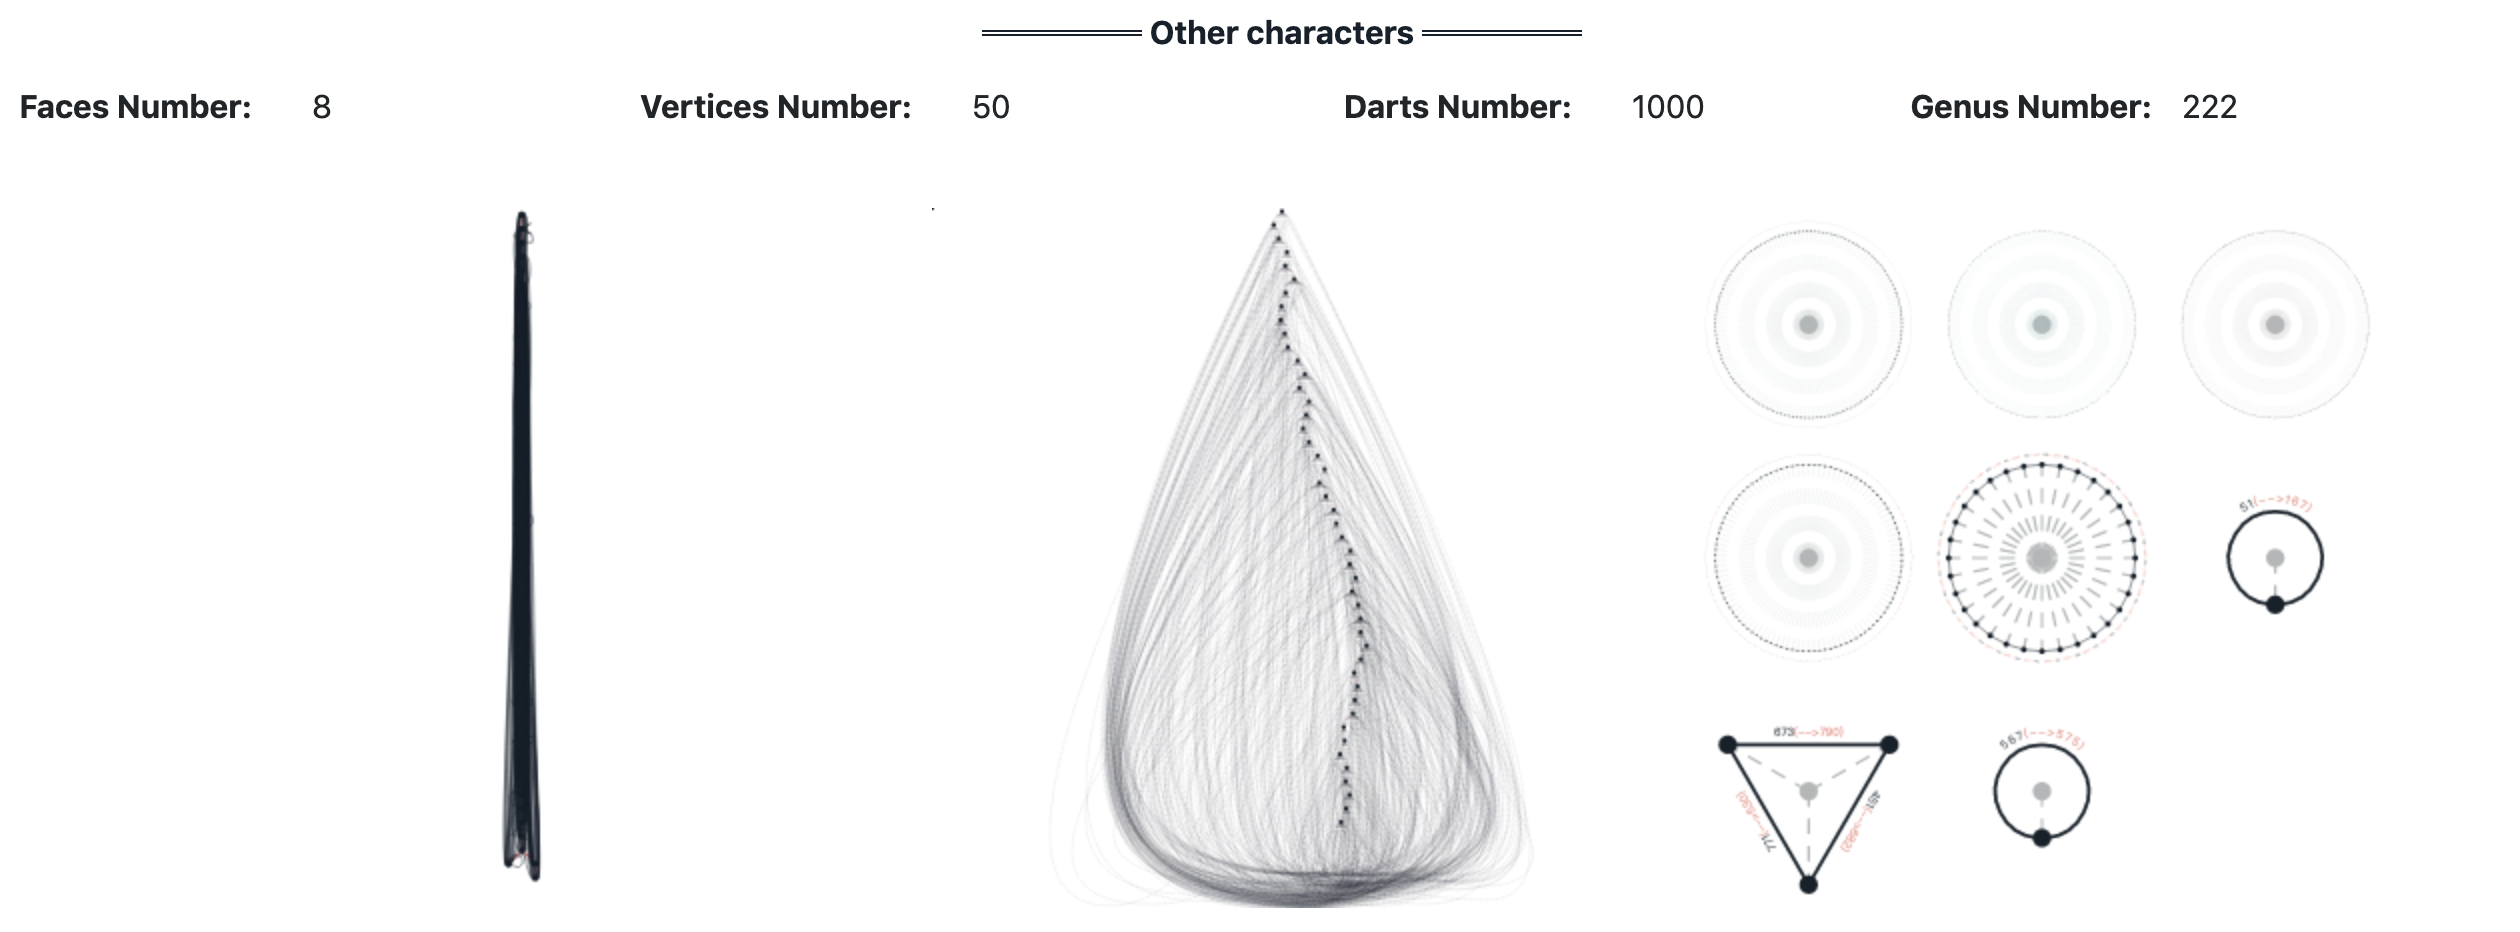
\includegraphics[width=1\textwidth]{../../image/clear3.png}
    \caption{A random map with 1000 darts.}
    \label{fig:figures:clear3}
  \end{figure}

  \subsection{Usability}
  All of the methods can generate a combinatorial maps successfully and the results are correct. For improving the aesthetics problem in first image, the highlight and tips are used to indicate the edges and vertices, though it just an assistant operation without changing the result. The highlight also occurs in the second method, since the edges are so slim that it difficult to spot the specific path of it in a large maps.  The SVG images can be zoomed through clicking the nodes in the them or some other operations with mouse like scrolling the mouse in the space. A reset button is used to recover the whole image.

\section{Testing the system}
After estimate the visualisation approaches, the system should be tested according to whether the specification in chapter 4 is satisfied. This also help to point out the bugs in the current system.

\subsection{Calculating of combinatorial maps}

\subsection*{Parsing the user input which is limited to the cycle notation. All the specifications in this item can be test under the `specific’ tab in the input area.}

\textbf{Correctness} Checked by entering a variety of valid strings, and making sure that the results match the cycle notation for each component. All tests are \textbf{passed}.

\textbf{Reliability} Checked by inputing different types of invalid strings. The error massage and simple examples occurs real time for the illegal string. As the mean time, if click `create’ button when the inputs are illegal, the output will give the corresponding error message rather than continue to generation of the maps. All tests are \textbf{passed}.

\textbf{Performance} Checked the corresponding text and images for a parsing in the output area are correct by hand. The test is \textbf{passed}.

\subsection*{Transforming cycle notation to one-line notation.All the specifications in this item can be test under the `specific’ tab and `random’ tab in the input area.}

\textbf{Correctness} Checked by entering different strings of  these two notations. The output should match the format of another notation. The test is \textbf{passed}.

\textbf{Performance} TChecked the corresponding text and images for a transformation in the output area are correct by hand. The test is \textbf{passed}.

\subsection*{Computation of faces by given the permutations of vertices and edges. This particularly depends on the equation \(\phi=\sigma o\alpha\). All the specifications in this item can be test under the `specific’ tab in the input area.}

\textbf{Correctness} Checked by entering variety vertices and edges permutations. The faces can be conducted in both notations. The test is \textbf{passed}.

\textbf{Performance} Checked the corresponding text and images for a face in the output area are correct by hand. The test is \textbf{passed}.

\subsection*{Generating a random combinatorial map by only given the number of darts (and vertices). All the specifications in this item can be test under the `random’ tab in the input area.}

\textbf{Correctness} Checked by entering different numbers of  darts and generating the graph which is connected successfully. The test is \textbf{passed}.

\textbf{Performance} Checked the text and images for each component in a map in the output area are correct by hand. The test is \textbf{passed}.

\subsection{Visualising combinatorial maps}

\subsection*{The tool using different methods to visualise the combinatorial maps. All the specifications in this item can be test at the bottom of the output area.}

\textbf{Correctness} Checked by judging whether the results of methods followed the constraints of the maps, that is, it must obey the orientation of each part.The whole structure must be connected and filled in the specific area without overflow. For the planar map, it must avoid the crossing as much as possible. All the tests are checked by hand, and the first two tests are \textbf{passed}. For the last test, the last method \textbf{passed}, while, for the first two, it \textbf{failed}.

\textbf{Clarity} Checked by making sure that users can have a clear mind when they look at the images immediately. This test \textbf{passed} for the last two methods and \textbf{failed} for the first approach.

\textbf{Performance} Checked by making sure that it shows the results in the right area and has an effective introduction. These test \textbf{passed}. Checked by creating a map in the limited time. This test \textbf{failed} when generating a large map with the huge number of vertices.

\textbf{Consistency} Checking by making sure the result of the certain method for a map must be the same at any time. These test \textbf{passed}.

\textbf{Aesthetics} Checked by showing tools to they others, and the receiving the feedback of the users. The most feedback is beautiful, colourful and clearly structural for the whole tool, but the result for the first approach looks a little terrible. Therefore, this test \textbf{passed} for the whole structure but \textbf{failed} for a specific result.

\subsection{Knowledge of combinatorial maps}

\subsection*{The tool aims to pass more information about combinatorial maps for whether they are beginners or experts in the relative area.  A introduction of the maps and tool is necessary.}

\textbf{Correctness} Checked by making sure the background of the combinatorial maps is correct and not misleading. The test \textbf{passed}.

\textbf{Performance} Checked whether each section of the introduction displays successfully and is there a introduction at the beginning of the visualiser page. The test \textbf{passed}.

% !TeX encoding=utf8
% !TeX spellcheck = en-US

\chapter{Further work}

\section{Achievements}

After testing the visualisation methods and the system in the section 6,most of the specifications are satisfied. The tool has the functions to pursue the drawing the combinatorial maps and visualising the vital features of the maps.
\begin{itemize}
    \item The introduction page and the head of the visualiser page help the users learn the combinatorial maps and know the basic structure of the tool.
    \item The tools support three kinds of input to satisfy different requirement of users. The existed examples which are the typical combinatorial maps help the user experience the whole process of the tool; people can also try and test their own sample using the specific input; if users have no much idea about the combinatorial maps, they can receive a random map from the random section by just enter the number of darts.
    \item The tool can parsing the users input and convert the input into an accessible format. It can also convert the one-line notation permutation to the cycle-notation, or reversely.
    \item The tool can calculate the faces with the help of edges permutations and vertices permutations according to the equation \(\phi=\sigma o \alpha\). It visualises all the permutations under both notations, as well.
    \item The visualiser can draw the tree structure using tree drawing algorithm. Under the tree model (spanning tree), the whole structure of combinatorial maps can be drew.
    \item A improved version of tree based methods also be implemented. This algorithm makes the result more transparent and tidy.
    \item Another method based on the dual of combinatorial maps is implemented, as well. The results of the method is clearer, but losing the connectivity between each face.
    \item To improve legibility of the visualisation, some interactive functions are added, for example, highlight the edges and vertices, indicating them for a tips and zooming the each canvas.
\end{itemize}

\section{Issues}

However, some issues occur in the testing results, which mainly around the visualisation approaches.
\begin{itemize}
    \item The methods under the spanning tree structure cannot avoid the crossing, especially for the first method which never avoid crossing at all. It even cannot generate a clear structure.
    \item The faces based method cannot shows the structure directly, that is to say, it needs an extra work for users to glue the faces together.
    \item When generating a large combinatorial maps with a lot of number of darts like 100 and the number of vertices is more than half of darts, the system might be blocked or delay generating the maps. The reason why this problem appears is the function that generates the permutation of vertices. Since, the probability of generating a \(VC\) contains empty members, as it was mentioned before, the empty elements cannot appear in the final result.
\end{itemize}

\section{Future improvement}

\subsection{Drawing methods}

\subsubsection{Tree based method}
Though there is an improved version of the first tree based method, but it can be better by itself. After the darts fixed, it can simulate the connecting approach in the second method by discussing different connection situations.  Through checking the directions of the two pre-connected darts to determine which side of space the curves might go through.

\subsubsection{Faces based method}
Gluing the faces is the next work of the method. The core idea is that if two darts of two faces are tied together,  rotating one of the faces clockwise so that the darts can fit together. Following the steps until all the faces are gluing together. In order to reestablish the surface which the maps embedded in, the folding method could be used.  However, the research of the folding algorithms stays in theoretical stage without the actual algorithmic process\cite{demaine2005survey} so that there is no effective measure for building a 3-dimensional or higher-dimensional surface from the 2-dimensional map.

\subsection{Interactions}

Additional interactions make the tool more entirely and practically.

\subsubsection{Save images}
The result of drawing is the SVG format. A saving functions to save the image into different format such as PNG, JPG and SVG. There is a method for convert the SVG format into the PNG in the JAVASCRIPT as the \textit{showInCanvas()} in the file \textit{type1.js}.  After that, the image can be download as the PNG.

\subsubsection{Animated operations}
The  zooming behaviour has been added into each result. One more operation, dragging is necessary too. Under the behaviour, people can drag and turn the faces in the last method to connect the them manually to make up for the lack of gluing faces. Meanwhile, it also enhances users expression of knowledges of equivalent for two maps.
\chapter{Project management}\
\section{Project structure}

This project is a continuation of the previous research. When I first came into contact with the concept of combinatorial maps, it was very vague to me.  The only information I know about it is the basic structure of  the maps, so that I just implement a method to visualise the map with the fundamental steps. With the successful implementation of the first visualisation method, I learned more about the maps and drawing graph. According to prior knowledges accumulated in the previous research, I was quite clear about the content and purpose of the project. The essential purpose is still using different methods to visualise the structure, but a tool produced to enhance the project integrity and practicality. It also used to validate the result of methods. After discussing the ideas with supervisor and writing the proposal, the structure of project is more clearly. The first step is generating the frame of the tool. Filled the tool with different visualisation methods.

Validating whether each unit of the tool works well and  testing if results of the approaches perform well according to the specification writing in the proposal. All tests through the strict constrains. At the beginning, the visualiser page was separated into two pages, one for trying the specific examples of users and a randomly generation as the another page. Some fixed examples were used to test the methods, so that the early work is to creating the format page. For reducing the time to input the same string every time, a typical examples item was supported.Due to the same process for generating maps, the page of producing the random maps was merged into the same page.

Though the project has been finished successfully, there are still some problems can be improved. So many time is using to check the related knowledges that it is no sufficient time to implement every ideas who might be pursued later.

\section{Project log}

The project log was submitted weekly on the canvas, which also can be seem in the Appendix B. The log help me to summarise the knowledges learned and recording the problems appeared in the project.  It gives me enough time to consider what should do next week, as well.

\section{Supervisor meeting}

Meeting with the Project supervisor held once a week, to know what I have done in the previous week and discuss the problems I met. A clearer mind and explicit direction have been achieved after the discussion.

\section{Version control}
The GitLa is used to control the version of the project. The log of the Git helps us know what changes in each push operations. It will store the latest version of project after implementing a new function or fixing the problems of the project.
\chapter{Conclusion}
Summarily, the project is to find different methods to visualise the combinatorial maps which is a topological structure. According to the previous research and work, the project set out to explore the layout of the map through searching the properties of combinatorial map. Firstly, it has the spanning tree and the structure can be produced based on the tree model. As the same time, many tree drawing algorithm can be used to build the tree structure. After implementing the first method, we found that the additional information is needed for the tree structure. The improved version of tree based method aims to strengthen the tree structure and makes the whole layout more transparent. Other than the spanning tree, another feature called dual of maps provide a new idea about the visualisation. Drawing faces and then gluing them. Unfortunately, the gluing method did not be implemented. From the whole project, the tool has already achieved the goals, though it still have some issues need to be fixed.

%%% -- end of main content

% -- bibliography --
% (must be placed _before_ appendix)
\IfPackageLoaded{biblatex}{
  \cleardoublepage
  \IfDefined{phantomsection}{\phantomsection}\label{sec:bibliography}
  \printbibliography[%
    heading=bibintoc, % (bibintoc, bibnumbered)
  ]	
}% end of bibliography

%% -- list of figures and tables --
\cleardoublepage\IfDefined{phantomsection}{\phantomsection}\label{sec:lof}
\listoffigures

% --- Appendix --- --- --- --- --- --- ---
\cleardoublepage\IfDefined{phantomsection}{\phantomsection}
\appendix
% Add `Appendix` to TOC
\addcontentsline{toc}{part}{\appendixname}
% must be _input_, otherwise the TOC entry is at the wrong place
% !TeX encoding=utf8
% !TeX spellcheck = en-US

%
% add files for appendix chapter here
\chapter{File Structure}
\label{chap:Appendix:A}
The appendix shows the structure of the project directory. The program can be started at any .html file in the html directory.
\section{root - \textbf{Main files}}
\label{sec:Appendix:root}
\begin{itemize}
    \item README.md: A readme file
\end{itemize}

\section{document \textbf{directory} - \textbf{Documents}}
\label{sec:Appendix:docs}

\begin{itemize}
    \item 1899855-Tingyu Huang-proposal.pdf: The proposal of the project.
    \item dissertation draft.pages: The draft of the dissertation.
    \item dissertation draft\_complete.pages: The content of dissertation.
    \item Drawer.pdf: The prorotype of the tool.
    \item latexthesistemplate directory: The Latex templete of the dissertaion. 
    \item Tingyu Huang-1899855.pdf: The dissertation of project.
\end{itemize}

\section{css \textbf{directory} - \textbf{Style of pages}}
\label{sec:Appendix:css}
\begin{itemize}
    \item index.css: The general style of the tool.
\end{itemize}

\section{html \textbf{directory} - \textbf{HTML files}}
\label{sec:Appendix:html}
\begin{itemize}
    \item index.html: The introduction page.
    \item type1.html: The visualiser page.
\end{itemize}

\section{javascript \textbf{directory} - \textbf{Source code}}
\label{sec:Appendix:js}
\begin{itemize}
    \item data.json: The file stores all the typical examples. (If the file cannot loading succesfully, the examples tab in the visualiser cannot be used. Since the limitation of the browser, a local servise is needed to resolve cross-domain issues, otherwise, the files cannot be read.)
    \item Drawing.js: All the implementation of visualisation.
    \item index.js: The initialization of introduction page.
    \item type1.js: The layout and data monitoring on visualiser page.
\end{itemize}

\section{image \textbf{directory} - \textbf{Images}}
\label{sec:Appendix:image}
The images used in the dissertaion and project.

\section{other \textbf{directories} - \textbf{Others}}
\label{sec:Appendix:other}
The library introduced in the project.
\chapter{Project log}
\label{chap:Appendix:B}
\textbf{week 1} This week mainly talk about the topics which were related to the combinatorial map. The first one is using different techniques to do the visualization of combinatorial maps and another one is to convert the pixels of images into combinatorial maps. For the first topic, there were two more methods can be used to visualize, using a spinning tree or using the third component faces of combinatorial maps.  As for the second topic, it needs more knowledge about it. All of these topics and approaches need me to do further research

The second task of the week was discussing which types of topics could I choose and how to perform the final work for the types. Two types were suitable to me, theory and software engineering, if I want to search the more methods to show the combinatorial map the first type might a good choice, however, if I can produce an interface to help the people know a lot about the combinatorial map, the second type is better. There is no doubt that this task is base on the first one. Hence, more information about the topics is needed to help make decisions and find the most appropriate project for me to do.

\textbf{week 2} The meeting this week had two parts, solving the problems in the proposal and identifying the details of the project.  After reading the proposal template, I found I was confusing about some items, for example, whether the project objective should be more specific or not. Therefore, the supervisor helped me to tackle the barrier. During this period, the approaches for dealing with the problem of the topic were settled, and we discussed if the ideas were feasible. Supervisor gave me more professional theoretical support and clearer research direction after listening to my description of the thoughts. 

\textbf{week 3} Discussing the details of the project through the proposal. First, a clear direction, since the project mainly cares about the approaches of visualization of combinatorial maps, it needs to involve all general combinatorial maps, rather than focus on the quite narrow type of maps like the maps based on the planar maps. As well,  certain the primary frame of the system via prototypes. 

\textbf{week 4} This week introduce the library and frame used to implement the designing of the sketch.

\textbf{week 5} Implement the sketch of the web page, and discuss the content of the report. The library for drawing the maps.

\textbf{week 6} The validating and parsing of the inputs and the supervise support some other idea for drawing the graph.

\textbf{week 7} Changing the structure of the pages, computing spanning tree and visualizing the permutation and cycles notations. Changing some terminology on pages.

\textbf{week 8} Implement drawing tree algorithm and visualizing tree-based combinatorial maps. Discussing faces-based algorithm and the methods to make the result clearer. Adding the useful introduction information to help freshman to understand the structure.

\textbf{week 9} Another tree-based method to avoid the cross problem. The problems occur in the project.

\textbf{week 10} Solving the problems occurred in the second tree-based method, and complete the method. Some suggestions about the layout of the page to collect all the type of inputs into one page.

\textbf{week 11} Finish the whole pages, fix the problem.

\textbf{week 12} Discussing details about the dissertation.

\textbf{week 13} Displaying the pages and discussing each section of the dissertation. Finishing the writing work.






% <------------------------

% add todo list (remove for final document!)
% \IfPackageLoaded{todonotes}{
  \clearpage
  \IfPackageLoaded{hyperref}{\phantomsection}
  \todototoc   % add to toc 
  \listoftodos % print to document
}


%%% document END %%%%%%%%%%%%%%%%%%%%%%%%%%%%%%%%%%%%%%%%%%%%%%%%%%%%%%%%%%%
\end{document}
%%%%%%%%%%%%%%%%%%%%%%%%%%%%%%%%%%%%%%%%%%%%%%%%%%%%%%%%%%%%%%%%%%%%%%%%%%%%
